% !TeX spellcheck = <fr_FR>
%%%% Modèle proposé par colin.avogadri@umontpellier.fr %%%%
%%%% 3 Février 2022 %%%%

\documentclass[english,12pt,a4paper]{book}

\usepackage[utf8]{inputenc}
\usepackage{mathpazo}
\usepackage[semibold]{sourcesanspro}
\usepackage{sectsty}
\allsectionsfont{\sffamily}
\usepackage[T1]{fontenc}
\usepackage[english]{babel}
\usepackage{amsmath}
\usepackage{amsfonts}
\usepackage{fancyhdr}
\usepackage{amssymb}
\usepackage{color} % où xcolor selon l'installation
\definecolor{Valentia}{RGB}{233,78,82}
\definecolor{Titleblue}{RGB}{114, 146, 162}
\usepackage{mdframed}
\usepackage{multirow} %% Pour mettre un texte sur plusieurs rangées
\usepackage{multicol} %% Pour mettre un texte sur plusieurs colonnes
\usepackage{scrextend} % Forcer la 4eme  de couverture en page pair
\usepackage{tikz}
\usepackage{graphicx}
\usepackage[absolute]{textpos} 
\usepackage{colortbl}
\usepackage{array}
\usepackage{geometry}
\usepackage{hyperref} 
\usepackage{minitoc}
\usepackage{microtype}
%\usepackage{refcheck}
\usepackage{easyReview}

\usepackage{framed}
\usepackage{latexsym}
\usepackage{url}
\usepackage{xcolor}
\definecolor{newcolor}{rgb}{.8,.349,.1}
\usepackage{subcaption}
\usepackage{stackengine}
\usepackage{svg}
\usepackage{wrapfig}
\usepackage{pdflscape}
\usepackage{afterpage}
\usepackage{capt-of}
\usepackage{longtable}
\usepackage{makecell}
\usepackage{titlesec}
\usepackage{float}
\usepackage{booktabs}
\usepackage{tabularx}
\usepackage{siunitx}
%\usepackage{breqn}
\usepackage{bookmark}

\sisetup{product-units=repeat}

\usepackage[backend=bibtex, backref=true, style=numeric]{biblatex} 
\bibliography{../references_terrain}


\setkeys{Gin}{width=\linewidth}

\renewcommand{\cellalign}{cl}
\newcolumntype{H}{>{\setbox0=\hbox\bgroup}c<{\egroup}@{}}




\newcommand{\R}{\mathbb{R}}
\newcommand{\norm}[1]{\left\lVert #1 \right\rVert}

\newcommand{\material}{\mathcal{M}}

\newcommand{\mass}{m}
\newcommand{\velFactor}{\nu}
\newcommand{\decay}{k}
\newcommand{\diffusion}{D}
\newcommand{\growthRate}{\gamma}
\newcommand{\fittingFunc}{\Gamma}
\newcommand{\fittingFuncObj}{\fittingFunc_{obj}}

\newcommand{\Water}{\mathcal{W}}
\newcommand{\Wuser}{\Water_\text{user}}
\newcommand{\Wsimu}{\Water_\text{simulation}}
\newcommand{\Wobj}{\Water_\text{objects}}

\newcommand{\terrain}{\mathcal{T}}
\newcommand{\height}{\mathcal{H}}
\newcommand{\depth}{\mathcal{D}}
\newcommand{\objects}{\mathcal{O}}
\newcommand{\environment}{\mathcal{E}}
\newcommand{\Wlevel}{\mathcal{L}}

\newcommand{\availableObjects}{\Tilde{\objects}}

\newcommand{\tEvent}{t_e}

\newcommand{\eps}{\varepsilon}


\newcommand{\erosionRate}{ \varepsilon }
\newcommand{\shearStress}{ \tau }
\newcommand{\criticalShearStress}{ \shearStress_{c} }
\newcommand{\velocity}{ \upsilon }
\newcommand{\capacity}{ C }
\newcommand{\maxCapacity}{ \capacity_{max} }
\newcommand{\density}{ \rho }
\newcommand{\particleDensity}{ \density_{p} }
\newcommand{\soilDensity}{ \density_{s} }
\newcommand{\particleMass}{ \mass_{p} }
\newcommand{\depositionRate}{ \omega } % Not the good notation, but I don't think there is a real notation
\newcommand{\real}{ \mathbb{R} }
\newcommand{\shearStressConstant}{ K }
\newcommand{\erosionStrength}{ K_{\erosionRate} }
\newcommand{\particleSize}{ R }
\newcommand{\settlingVelocity}{ w_s }
\newcommand{\fluid}{ f }
\newcommand{\fluidDensity}{ \density_\fluid }
\newcommand{\fluidVelocity}{ \velocity_\fluid }
\newcommand{\buoyancy}{ B }
\newcommand{\gravity}{ G }
\newcommand{\erosionAmount}{ q_{detachment} }
\newcommand{\depositAmount}{ q_{deposit} }
\newcommand{\totalErosion}{ Q }
\newcommand{\extForce}{ F_{ext} }
\newcommand{\capacityFactor}{ C_{factor} }

\newcommand{\inset}[3][0.2\linewidth]{\noindent\stackinset{r}{0.1cm}{b}{0.1cm}{\colorbox{white}{\includegraphics[width=#1]{#3}}}
	{\includegraphics[width=\linewidth]{#2}}}

\usepackage[Sonny]{fncychap} %% Pour changer le style de chapitre
\pagestyle{fancy}
%\fancyhf{}
%\fancyhead[RE,RO]{\chaptername \thechapter . \chaptermark}
\fancyhf{}
\fancyheadoffset{0.005\textwidth}
\fancyhead[LE]{\thepage}
\fancyhead[RE]{\nouppercase\leftmark}
\fancyhead[RO]{\thepage}
\fancyhead[LO]{\nouppercase\rightmark}
%%%%%%%%%%%%%%%%%%%%%%%%%%%%%%%%%%%%%%%%%%%%%%%%%%%%%%%%%%%%%%%

\dominitoc
\let\oldminitoc\minitoc
\def\minitoc{
	\oldminitoc
	\noindent\textbf{\hyperlink{tocpage}{Back to summary}} \\
}
\makeatletter\@addtoreset{chapter}{part}\makeatother%

\begin{document}
	
\pagenumbering{roman}


\begin{titlepage}
	
	\newgeometry{left=2.5cm, bottom=3cm, top=2cm, right=2.5cm}
	
	\tikz[remember picture,overlay] \node[opacity=1,inner sep=0pt] at (73.6mm, -124.25mm){
\includegraphics{images/PhD_Couverture_Fond.pdf}};
	
	{\fontfamily{phv}\fontseries{mc}\selectfont
		%*****************************************************
		%******************** TITRE **************************
		%*****************************************************
		\centering
		\color{Valentia}
		\fontsize{18}{13}\selectfont
		\textbf{THÈSE POUR OBTENIR LE GRADE DE DOCTEUR\\ DE L'UNIVERSITÉ DE MONTPELLIER}
		
		\normalsize
		\color{black}
		
		\bigskip
		\textbf{En informatique}
		
		\bigskip
		\textbf{École doctorale I2S}
		
		\bigskip
		\textbf{Unité de recherche LIRMM}
		
		
		\color{Titleblue}
		\fontsize{17}{20.4}\selectfont
		\vspace{2cm}
		\textbf{Génération procédurale d'environnements 3D sous-marins\\Procedural generation of 3D underwater environments}
		
		%*****************************************************
		
		\vspace{4cm}
		\fontsize{15}{18}\selectfont
		\color{black}
		\textbf{Présentée par Marc HARTLEY \\
			le [XX mois année]}
		
		\bigskip
		\fontsize{13}{15.6}\selectfont
		\textbf{Sous la direction de Christophe FIORIO, 
			Noura FARAJ \\
			et Karen GODARY-DEJEAN}
		
		\vspace{1.5cm}
		\normalsize
		\textbf{Devant le jury composé de}\\
		\bigskip
		\fontsize{10}{12}\selectfont
		\vspace{1.5mm}
		\begin{tabularx}{\textwidth}{l X r}
			% \textbf{Mme. CANI Marie-Paule} & Professeur des universités & [Affiliation] & Rapporteur \\
			% \textbf{M. GUÉRIN Éric} & Professeur des universités & [Affiliation] & Rapporteur \\
			% \\
			% \textbf{M. BOUDON Frédéric} & Maître de conférence & CIRAD-UMR AGAP-Institut & Examinateur \\
			% % \textbf{Prénom NOM} & [Titre] & [Affiliation] & [Rôle] \\
			% \\
			% \textbf{M. FIORIO Christophe} & Professeur des universités & Université de Montpellier & Directeur de thèse \\
			% \textbf{Mme. FARAJ Noura} & Maître de conférence & Université de Montpellier & Co-directeur de thèse \\
			% \textbf{Mme. GODARY Karen} & Maître de conférence & Université de Montpellier & Co-directeur de thèse \\

			\textbf{Mme. CANI Marie-Paule} & Professeur des universités & Rapporteur \\
			\textbf{M. GUÉRIN Éric} & Professeur des universités & Rapporteur \\
			\\
			\textbf{M. BOUDON Frédéric} & Maître de conférence & Examinateur \\
			% \textbf{Prénom NOM} & [Titre] & [Rôle] \\
			\\
			\textbf{M. FIORIO Christophe} & Professeur des universités & Directeur de thèse \\
			\textbf{Mme. FARAJ Noura} & Maître de conférence & Co-directeur de thèse \\
			\textbf{Mme. GODARY Karen} & Maître de conférence & Co-directeur de thèse
		\end{tabularx} 
		
		%************************************
		%**  LOGO  UNIVERSITÉ
		%*****************************************************
		\vspace{\fill}
		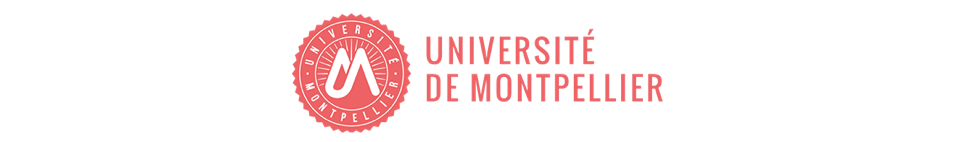
\includegraphics[scale=1]{images/PhD_Couverture_LogoUM.png}
		\vspace{-15mm}}
\end{titlepage}

%%%%%%%%%%%%%%%%%%%%%%%%%%%%%%%%%%%%%%%%%%%%%%%%%%%%%%%%%%%%%%
\newgeometry{top=2cm, bottom=2.5cm, left=2cm, right=2cm}
\setcounter{tocdepth}{3}
\tableofcontents
\addtocontents{toc}{\protect\hypertarget{tocpage}{}}
%\listoffigures \addcontentsline{toc}{chapter}{List of Figures} \mtcaddchapter                     %new code
%\listoftables \addcontentsline{toc}{chapter}{List of Tables}   \mtcaddchapter                     %new code

\clearpage
\pagebreak

\section*{Abstract}

This thesis, entitled \textit{"Procedural terrain generation for underwater environments"}, explores the specialised area of procedural terrain generation, specifically targeting underwater settings. Procedural terrain generation remains a vibrant research area within computer graphics, particularly as advancements in simulation, rendering, and interaction techniques have fostered increased collaboration with terrain experts across various disciplines.

Virtualising the physical world enables users to observe and interact with it in ways that enhance understanding and break down the boundaries between scientific fields. Terrain science, by its nature, brings together a diverse range of experts, including geologists, oceanologists, physicists, meteorologists, biologists, roboticists, computer scientists, and 3D artists. This thesis focuses on involving users in the creation of virtual worlds through fast and controllable algorithms, with a particular emphasis on underwater environments.

The thesis is structured into three parts, guiding the reader from the initial design of a landscape through to its 3D modelling and final refinement.

In the first part, we introduce a formal approach to terrain design, allowing environments to be conceived in semantic terms, abstracting away from the complexities of 3D geometry and data structures.

The second part focuses on translating these conceptual environments into 3D form. We present new models for generating and modelling coral reef islands and karst networks.

Finally, in the third part, we concentrate on enhancing the realism of these 3D terrains through physical simulations of erosion processes. We demonstrate a flexible and controllable method for simulating the long-term effects of water and wind on both terrestrial and marine landscapes.







% This thesis, entitled \textit{"Procedural terrain generation for underwater environments"}, as its name suggests, focuses on the topic of procedural terrain generation with the specificity to tackle the tackle underwater environments. Terrain generation is still an open research area in computer graphics as, with the emergence of simulation, rendering, and interaction techniques, the entire field is experiencing increased collaboration with terrain experts. 
% Virtualization of the physical world helps users to see and manipulate it, allowing for a better understanding of it and bringing together numerous experts, gradually breaking down the boundaries of scientific disciplines. 
% Terrain science brings together, in almost a direct manner, geologists, oceanologists, physicists, meteorologists, biologists, roboticists, computer scientists, 3D artists, and more. We focused our work on the inclusion of the user in the generation process of virtual worlds through fast and controlable algorithms, with the possibility to dive underwater.

% This thesis is divided into three parts, guiding the user from the design of a landscape, its 3D modeling, until its finalization, step by step.
% Firstly, we will propose a formalization of terrain designing, allowing for the conception of environments in a semantic sense, abstracting away from 3D geometry and data structures.

% Secondly, we will see how to give 3D form to these environments. We will propose new models for the generation and modeling of coral reef islands and karst networks.

% In the third part, we will focus on adding realism to 3D terrains through physical simulations of erosion processes. We will demonstrate a flexible and controllable method to imitate the long-term effects of water and wind on both terrestrial and marine landscapes.

\textbf{Keywords:} terrain representation, procedural generation, physical simulations, user interaction

% \section*{Résumé}
% Cette thèse porte sur le thème de la génération procédurale de terrains en milieux sous-marins. La génération de terrain est un domaine de recherche encore ouvert en informatique graphique car, avec l'emergence des techniques de simulation, de rendu et d'interaction, le domaine entier connait un accroissement de collaboration avec les experts terrains. Amener le monde physique dans un ordinateur et permettre à son utilisateur de voir et manipuler ce monde virtuel permet de mieux le comprendre et de réunir de nombreuses experts ensemble, brisant petit à petit les frontières des disciplines scientifiques. La science des terrains rassemble, de manière presque directe, géologues, oceanologues, physiciens, météorologues, biologistes, roboticiens, informaticiens, artistes, etc... 

% Cette thèse se divise en trois parties amenant l'utilisateur de la conception d'un paysage jusqu'à sa finalisation, étape par étape, en gardant le control en tout point. 
% Premièrement, nous proposerons une formalisation d'esquissage de terrains, permettant la conception d'environnements dans un sens sémantique, permettant de s'abstraire de la géometrie et de structures de données. 

% Secondement, nous verrons comment donner forme 3D à ces esquisses. Nous proposerons de nouveaux algorithmes pour la génération et modélisation d'iles coralliennes et de réseaux karstiques.

% En troisième partie, nous nous interesserons à l'ajout de réalisme sur terrains existants au travers de simulations physiques de processus d'érosion. Nous montrerons une méthode flexible et controlable pour imiter les effets de l'eau et du vents à très long terme sur un paysage terrestre et marin.

% \textbf{Mots-clés :} représentation de terrain, génération procédurale, simulations physiques, interaction utilisateur

\mainmatter
\pagenumbering{arabic}

\chapter{Introduction}
\label{chap:introduction}
\minitoc

- ...

\section{Génération procédurale}
\label{sec:introduction_procedural-generation}
- ...

\subsection{Définition}
- ...

\subsubsection{Définition officielle}
- ...

\subsubsection{Ma définition}
- ...

\subsection{Historique}
- ...

\subsection{Modèles représentés}
- ...

\subsubsection{Bruit}
- ...

\subsubsection{Automates cellulaires}
- ...

\subsubsection{Réseaux de neuronnes}
- ...

\subsubsection{Modélisation de phénomènes physiques}
- ...

\subsection{Interaction utilisateur}
- ...

\subsubsection{Balance réalisme-rapidité-control}
- Principale problématique de la génération de terrains \\
- Explication réalisme \\
** Paysages générés sont proches de ce qui se retrouve dans la réalité \\
** La génération intègre les processus naturels pour être réaliste \\
** Demande beaucoup de simulations physiques, de connaissances experts \\
** Utile dans les applications de simulation de catastrophes naturelles, par exemple \\
- Explication rapidité \\
** Génération la plus rapide possible, l'objectif étant la génération en temps-réel \\
** J. Gain classifie: temps-réel (< 30ms), interactif (< 3s), proche de interactif (< 5min) et long terme. \\
** Utile dans les jeux vidéos "infinity-scroll", par exemple\\
- Explication control \\
** Cherche à satisfaire les demandes de l'utilisateur \\
** Grosse problématique étant les demandes "impossibles" de l'utilisateur. \\
** Utile dans la plupart des applications de la gen. proc. : accélerer le travail d'artistes, par exemple \\
- ...

\subsubsection{Régénération}
- Actions manuelles \\
- Problématiques de la régénération \\
** Quoi regénérer ? \\
** Comment régénérer ? \\
** Problèmes des interactions utilisateur ? \\
- Fichier de stockage d'actions JSON (?)
- ...



\section{Representation de terrains}
\label{sec:introduction_terrain-representations}
- ...

\subsection{Terrains 2.5D}
- ...

\subsubsection{Cartes de hauteur}
- ...

\subsubsection{Fonctions de hauteur}
- ...

\subsection{Terrains 3D}
- Besoin de notions 3D \\
** Information geologique \\
** Données volumiques \\
- ...

\subsubsection{Problématiques principales}
- Mémoire \\
- Visualisation \\
- Modifications \\
- Conversion entre representations \\
** Pertes d'informations \\
*** Propagation d'erreur sur la géométrie (approximations sur les normales, résolution Z, surface, etc...) \\
*** Perte d'informations sous-terraines \\
- ...


\subsubsection{Types, définitions, avantages, inconvéniants}
- Grilles de voxels \\
- Piles de matériaux \\
- Maillage \\
- Surfaces implicites \\
- ...

\subsection{Autres modèles}
- Notion de sémantique \\
- ...

\subsection{Paysages sous-marins}
- Données 3D \\
** Paysages coralliens remplis de vide \\
** Beaucoup de cavités (caves, grottes, reseaux karstiques) \\
- Données interdisciplinaires \\
** Plutôt commun avec generation de terrains\\
** => validation géologique avec des experts \\
** Pour sous-marin, \\
*** Moins d'experts, \\
*** Plus d'incertitudes \\
*** Plutôt basé sur des observations \\
*** Peu de données (paysages coralliens < 0.1\% des océans), pour gros impact biologique (25\% biodiversité marine) \\
** Mélange de géologie, biologie, hydrologie et physique (des fluides, notamment) \\
- Besoin de multi-échelles \\
** Pas limité au sous-marin \\
** Intégrer de gros éléments (montagnes) avec des petits éléments (végétation). \\
** LOD \\
- ... 

\subsubsection{Simulations de fluides}
- Très important dans génération procédurale de terrain \\
- Permet de justifier la géophysique d'une simulation/génération. \\
- Solutions assez rapide en 2D (PIC, FLIP, Stable Fluids, SPH, etc...) \\
- Mais devient beaucoup plus lourd et memoire intensif en 3D
- ...



\section{Paysages coralliens (partie biologique)}
\label{sec:introduction_biology}
- Historique découverte des récifs de corail \\
- Iles, barrières, atolls \\
- Théories des atolls \\
- Utilité dans la biodiversité \\
- Menaces, protection, importance de les comprendre \\
- ...

\section{Géométrie et structures de données}
\label{sec:introduction_geometry-datastructures}
- Présentation des structures utilisées \\
- ... 

\subsection{Géométrie}
- ... 

\subsubsection{Points}
- Definis dans l'espace 3D sous forme $\left( x, y, z \right)^T$. \\
- Quand projeté en 2D, $z = 0$ implicite. \\
- Représentés dans le manuscrit comme: $\p \in \R^3$ \\
- ...

\subsubsection{Courbes}
- Fonction paramétrique $\curve: [0, 1] \to \R^3$. \\
- Sauf mention contraire, utilisation de Centripetal Catmull–Rom spline [CITE CATMULL 1974]: \\
** Let $\p_i$ denote a point. For a curve segment $\curve$ defined by points $\p_0$, $\p_1$, $\p_2$, $\p_3$ and knot sequence $t_0$, $t_1$, $t_2$, $t_3$, the centripetal Catmull-Rom spline can be produced by:
\begin{align}
    \curve(t) = \frac{t_2 - t}{t_2 - t_1} B_1 + \frac{t - t_1}{t_2 - t_1} B_2
\end{align}
where
\begin{align}
    B_1(t) &= \frac {t_2 - t}{t_2 - t_0} A_1(t) + \frac{t - t_0}{t_2 - t_0} A_2(t) \\
    B_2(t) &= \frac{t_3 - t}{t_3 - t_1} A_2(t) + \frac{t - t_1}{t_3 - t_1} A_3(t) \\
    A_1(t) &= \frac{t_1 - t}{t_1 - t_0} \p_0 + \frac{t - t_0}{t_1 - t_0} \p_1 \\
    A_2(t) &= \frac{t_2 - t}{t_2 - t_1} \p_1 + \frac{t - t_1}{t_2 - t_1} \p_2 \\
    A_3(t) &= \frac{t_3 - t}{t_3 - t_2} \p_2 + \frac{t - t_2}{t_3 - t_2} \p_3
\end{align}
and
\begin{align}
    t_{i + 1} = \sqrt{ \left(x_{i+1} - x_i \right) + \left(y_{i+1} - y_i \right) +  \left(z_{i+1} - z_i \right)}^\alpha + t_i
\end{align}
in which $\alpha$ ranges from 0 to 1 for knot parameterization, and $i = 0, 1, 2, 3$ with $t_0 = 0$. For centripetal Catmull-Rom spline, the value of $\alpha$ is 
0.5. When $\alpha = 0$, the resulting curve is the standard uniform Catmull-Rom spline; when $\alpha = 1$, the result is a chordal Catmull-Rom spline. \\
** We will keep $\alpha = 0.5$ for all the work in this manuscript, as it felt like a good compromise between smoothness and control on the curve. The value of $\alpha$ has not been studied deeply. \\
- Avantages: Centripetal Catmull-Rom spline has several desirable mathematical properties compared to the original and the other types of Catmull-Rom formulation. First, it will not form loop or self-intersection within a curve segment. Second, cusp will never occur within a curve segment. Third, it follows the control points more tightly. [COPIE COLLE WIKIPEDIA] \\
- De plus, nous n'utilisons pas de "handles" (invisible control points) like for Bézier curves. At the cost of a little user control, I feel the that the use is simplified. \\
- Le calcul des derivées premières et secondes (tangeante et normale) sont rapides à calculer. \\
- ...

\subsection{Structures de données}
- ...

\subsubsection{Grilles 3D}
- Dans ce manuscrit, toutes grilles 3D définies en float32 signé. \\
- Pas optimial, notamment pour representé voxels binaires (utilisation de 32x plus de mémoire et calcul que nécessaire), mais flexible... \\
- Grilles de voxels stockées sous forme de listes de sous-grilles 3D ("modifications locales") pour naviguer en undo-redo. Evaluation d'une cellule par somme des sous-grilles. \\
- ...


\section{Création du prototype}
\label{sec:introduction_prototype}
- C++23 et Qt5.12 \\
- OpenGL 4.6 et GLSL \\
- Marching Cubes sur geometry shader \\
** Mauvaise idée, mais justifier le pourquoi \\
- Rendus :\\
** Avec le prototype : \\
*** Marching Cubes sur geometry shader \\
*** Triplanar texture \\
*** Résultats temps-réels \\
*** Textures selon matériaux \\
** Avec Unreal Engine 5 : \\
*** Maillages statiques \\
*** Ajout de végétation procédurale avec plugin [NOM DU PLUGIN] et océan avec [NOM DU PLUGIN] \\
** Avec Blender 4.1 \\
*** Maillages statiques \\
*** Utilisation de scripts plus facile \\
- ...

\section{Contributions et plan}
\label{sec:introduction_contribution-plan}
- Ordre chronologique de la génération de terrains \\
- Propose une representation abstraite à mi-chemin entre informatique et expertise terrain \\
** Offrant une généralisation du type de paysage souhaité (sous-marin, mais aussi terrestre) \\
- Proposition de nouveaux types de paysages (karsts et iles coralliennes) \\
** Conservation de la notion de parcimonie (volumes implicites) \\
- Propose une méthode de simulation d'érosion par particules \\
** Agnostique de la représentation de terrain \\
** Légère, rapide, simple d'implémentation \\
- Objectif de garder un maximum de controle pour l'utilisateur \\ 
** Dans le processus de génération, mais aussi pour rectifier en amont des détails

\subsection{Sémantique}
- Travail orienté sur la génération sous-marine \\
- Collaboration avec un biologiste marin \\
- 

\subsection{Modélisation}
- Génération de certains éléments de paysages encore nouveaux (karsts à référer à Axel Paris, mais iles coralliennes nouveau) \\
- Réseaux karstiques représentés de manière hautement user-friendly \\
** Voir les karsts comme un graphe orienté acyclique => proche de la structure arbre \\
** Augmentation de la méthode pour génération fractale avec cycles (génération en plusieurs itérations) \\
- Iles coralliennes en utilisant une interprétation de la théorie de Darwin \\
** Basée sur des observations \\
** Basé sur des carnets de voyages

\subsection{Amplification}
- Augmenter le réalisme par l'ajout de détails \\
- Méthode d'érosion basé sur l'utilisation de particules \\
** Généralisation pour flexibilité \\
** Rapidité, parallelisation \\
- Vers une méthode d'érosion continue.

\part{Representation sémantique}

\graphicspath{ {./Chapitre1/} }

\chapter{Generation de terrain sémantique}
\label{chap:semantic-representation}
\minitoc
\teaser{
	 \includegraphics[width=0.9\linewidth]{Figures/Render/figureTeaser.png}
	 \centering
	  \caption{Our method can produce different scenes including coral islands and canyons at multi-scale using environmental objects to represent terrain features.}
	\label{fig:semantic-representation_teaser}
	}

\section{Introduction}
\label{sec:semantic-representation_introduction}
Automated terrain generation is a key component of natural scene digital modeling for animated movies and video games. Many landscapes have been studied and are synthesised with more and more realism. 
Different processes can be used and combined to achieve these scenes: fractal terrains \cite{Musgrave1989,Prusinkiewicz1993a}, erosion simulation \cite{Cordonnier2023, Mei2007}, manual modeling \cite{DeCarpentier, Guerin2022}, geological simulation \cite{Cortial2019,Cordonnier2017a}, ... The high quality of synthesis for such environment is due to the possibility to observe these environments from many point of views: long-distance gazing, hiking on mountains, remote sensing, aerial imaging, ... 
Thanks to the quality of the digital modeling, the entertainment industry display often breathtaking land scenes.

Underwater scenes are rarely created in these media for multiple reasons: these environments are not completely understood and mastered as much as land environments because they are difficult to access, we lack the capacity to see them at a larger scale (unlike mountains for example) and the underlying process that forms these landscapes are much more complex to simulate.

These limitations cause animated movies and video games studios to avoid as much as possible underwater environments. 

However, these environments are important for the study of biology, geology, and, by extension, robotics. Due to the complexity, limitations and danger of underwater human operations, underwater robots are more and more used for marine environment monitoring\cite{Maslin2021, Williams2016, Dunbabin2020, Palmer2021}. Yet the validation process of such underwater robot is expensive, with heavy logistic, and it is often  impossible to find the appropriated environment to test the system. Thus, underwater robotics requires simulation capacities, to be able to test the robot's algorithms in very specific environment and conditions. But for now, roboticians are lacking the capacity to test on realistic virtual scenes, and so only test them on synthetic scenarios that do not correlate with real world terrains. For that, they need to manipulate more precisely the characteristics of the underwater environment, at different scales.

The difficulties to visualize and study the underwater environments on a large scale at the same time as a small scale is an obstacle to the procedural generation and simulation of scenes that are coherent in these two different scales. 
A solution to this problem could be a bottom-up approach, simulating at the smallest scale the behaviour of all the elements of the environment. Computing such a simulation in order to generate an entire ecosystem is an near-impossible task due to time and memory complexity. 

The method we propose provides a way to procedurally generate environments on multiple scales without introducing such complexity by using a sparse representation of the environment using environmental objects.
The environmental objects only have access to local values of the environments to spawn, grow and die. The use of local interaction with environment values removes the need for complex interconnections between all elements of the terrain, providing a parallelisable generation process at large to small scales.
Defining environmental objects of the terrain as parametric models based on point, curve or region skeletons provides a lightweight representation of the terrain that the user can interact with. The interaction with the simulation process is still a difficult task \cite{Smelik2014}.
Our method does not aim for a visually realistic generation, but for a plausible terrain depending on geological and biological constraints, guided by the user. Using state of the art modeling of the geometry of the environmental objects of the terrain could achieve realistic results. We illustrate the method through the generation of coral islands and reefs.

Our main contribution are the introduction of a sparse representation of the terrain elements as environmental objects, the use of fitting functions to incorporate biological rules in the simulation process avoiding physic simulation and an interactive simulation based on geological events for underwater landscapes.


\section{Related works}
\label{sec:semantic-representation_related-works}
Procedural terrain generation has been heavily studied for the last 40 years \cite{Galin2019}. Researches in this topic try to find new solutions to compromise between realism, user control and efficiency \cite{Gain2009}. Using fractal noise parametrized to resemble real landscape has been an important first step \cite{Musgrave1989} as it's a fast and light solution to generate procedurally the appearance of mountains. The lack of user control pushed newer works toward the use of controlled noise by including real DEM in the process through learning \cite{Kapp2020, Brosz2007}, while the rise of deep learning technologies gave higher control to the user through sketches \cite{Guerin2017, Talgorn2018}. \\
By including expert knowledge of tectonic process and subsurface geology, some algorithms tend to get more realistic \cite{Patel2021, Cortial2019, Michel2016}. \\
While these algorithms are able to generate large-scale landscapes, the finer details of the terrain is often computed by the use of erosion simulation \cite{Cordonnier2023, Schott2023, Paris2019}. This process can be expensive in time but results in more plausible surfaces.

All the algorithms aim to reproduce plausible relief in terrestrial landscapes, mostly limited to alpine landscapes, but a lack of research can be found in almost all other biomes. Underwater landscapes generation, for example, has been almost completely absent from literature for many reasons: the difficulty of accessing the area, the lack of visibility under water and the complex physics of underwater geology and biology make the algorithms adapted for this environment scarce. \\
The majority of the ocean floor can be represented as a fractal terrain \cite{Mareschal1989}. While stochastic noise can be sufficient to model the ocean floor, this process won't cover areas with the biggest biomass, near shallower waters such as near coasts and islands. \\
Due to the impossibility to observe the large-scale and the small-scale of underwater environments, some works related to geology model large structures like the profile shape of the coral reef \cite{Bosscher1992}, simulate its surface growth \cite{Li2021}, or use procedural algorithms for single polyp \cite{Abela2015}. We however don't have a mix of the different scales, and neither methods take into account the environment such as the topography or the interaction of different terrain elements. This is mainly due to the fact that the evolution time for each scale varies from a span of weeks to thousands of years.

In an ecosystem, any element of the system has an impact on their surrounding. Simulating each physical properties such as shading, heat, humidity may require enormous computation power. By considering these properties as scalar fields surrounding the whole scene, and that elements of the terrain affect locally the scalar fields, we can simplify the computation of the physical properties of the environment \cite{Grosbellet2016, Guerin2016a}. This process provides a scalable system from which scene details are rendered in a plausible way. In a similar way, other works represent the wind flow as a composition of local vector fields \cite{Wejchert1991}, avoiding complex fluid simulation while providing user control in a lightweight model. We extend these works by incorporating a time-evolution system such that the scene can be dynamic.


\section{Method}
\label{sec:semantic-representation_method}
The overall pipeline of the method is based on simple incremental generation like most rule-based systems. In this type of system, the final state is defined either by reaching equilibrium, or by verifying specific conditions, such as a maximum number of iterations. 
We define our pipeline in three phases (Figure~\ref{fig:semantic-representation_pipeline}): the initialization phase that describe the generation and simulation rules, the iterative phase generating populating the terrain with our environmental objects and finally the output.


\subsection{Pipeline overview}
\label{sec:semantic-representation_pipeline}

\begin{figure*}
    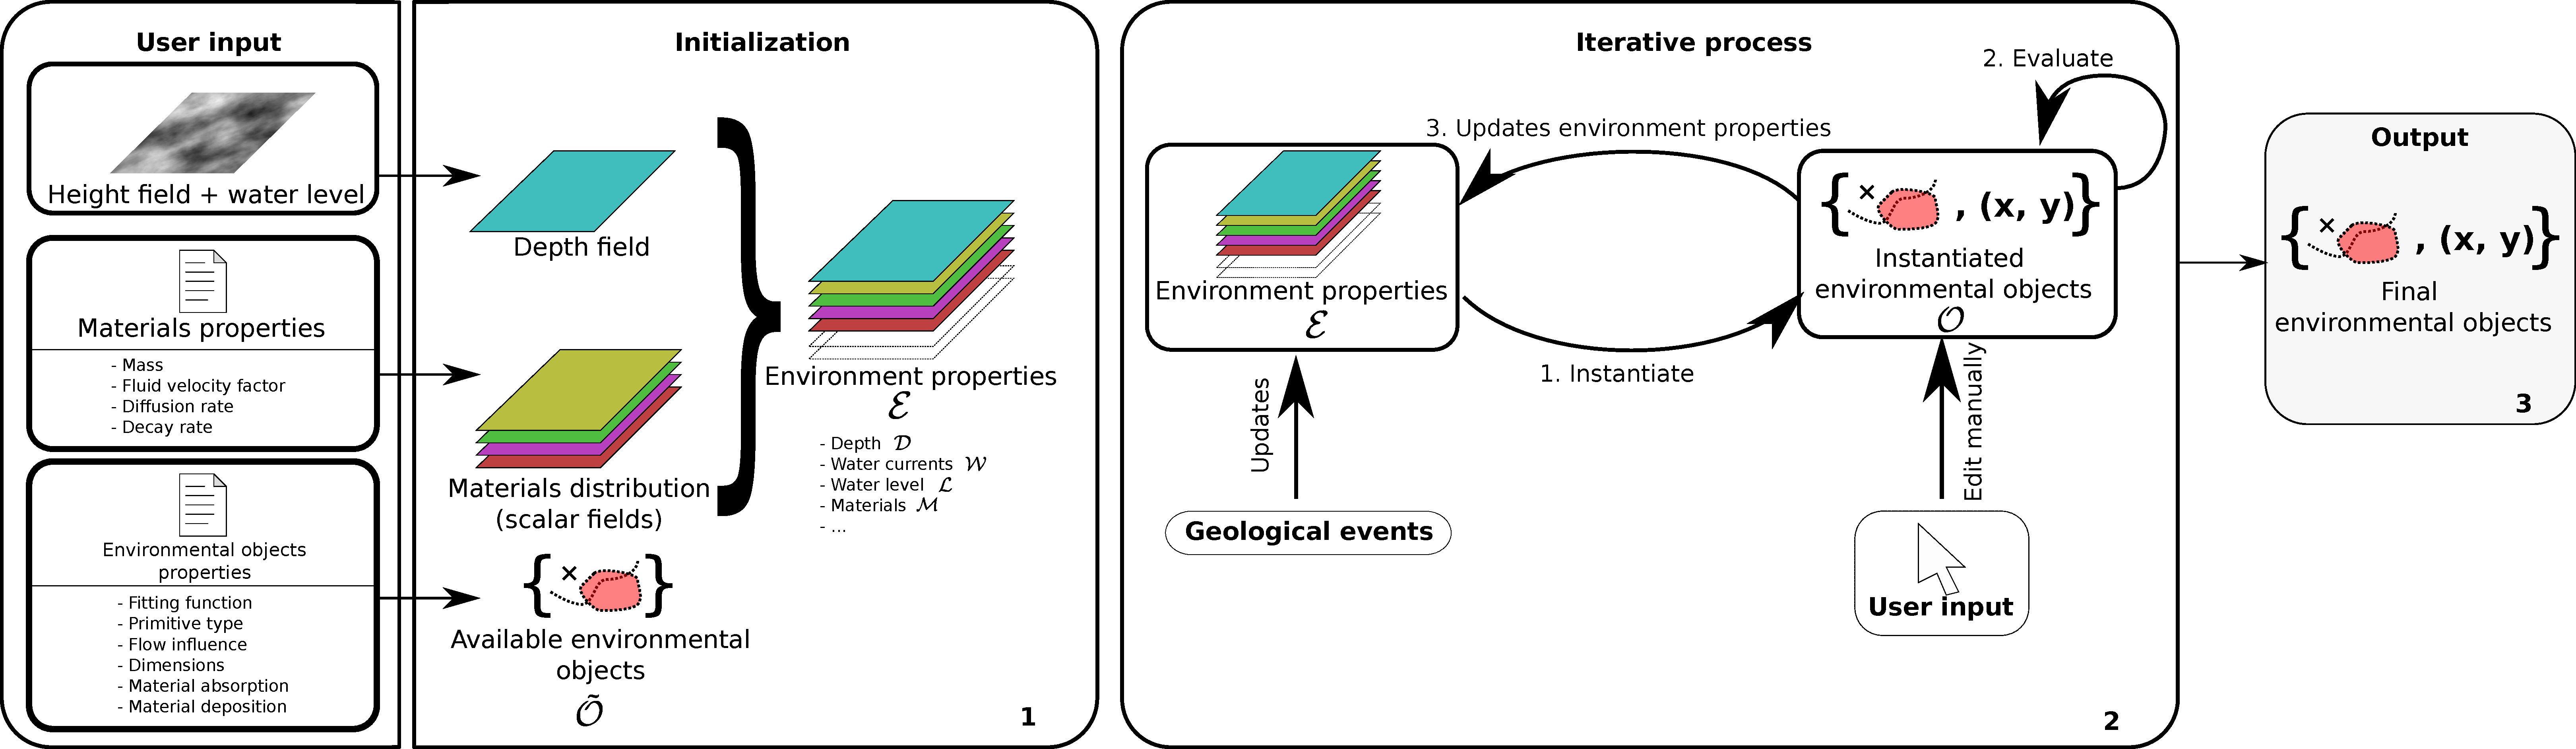
\includegraphics{Figures/pipeline.pdf}
    \caption{Overview of the pipeline of the method. The user provides as input an initial height field and sets the water level, as well as a definition of the materials properties and environmental objects properties that will be used in the iterative process. These inputs are initialized as an initial set of environmental objects and scalar fields that represents the environment values. In the iterative loop, new environmental objects are instantiated using the current state of the environment at their optimal position. The existing environmental objects in the terrain reevaluate their fitting function to grow or die and update the environment values locally. At each iteration, geological events can update the environment values, while the user can interact directly with the environmental objects. The result of the whole process is a set of environmental objects which is a sparse representation of the elements of the scene. }
    \label{fig:semantic-representation_pipeline}
\end{figure*}

The generation of the terrain is initialized using an initial height field $\height$ and a water level $\Wlevel$. The height field provides variation on the depth $\depth$, which can influence the generation process of the scene. We set $\depth = \height - \Wlevel$. \\
The list of available environmental objects $\availableObjects$, representing the different elements that can be present in the scene, are provided with their properties: type, size, generation rules, growing conditions and effects on the environment values (Section~\ref{sec:semantic-representation_environmental-objects}). \\
Finally, different materials can be defined with their properties such as diffusion speed, mass, damping factor and influence from the water currents. Materials distributions are represented as a scalar field $\material: \R^2 \to \R$ and water currents as a vector field $\Water: \R^2 \to \R^2$ that can be evaluated by the environmental objects of the scene to simulate their growth and spawn at the most probable position. The environmental properties $\environment = (\depth, \Water, \Wlevel, \material)$ is composed of depth, water currents, water level and materials distribution information at any point of the terrain (Section~\ref{sec:semantic-representation_communication}). \\
The definition of environmental objects' properties and environment properties is done with field experts, providing the pertinent parameters required to model the evolution of the terrain elements using expert knowledge (Section~\ref{sec:semantic-representation_biology}). Additional properties can easily be added to the environment properties $\environment$ in order to fit to the experts needs, such as atmospheric pressure, humidity, temperature, ... \\
The generation phase can optionally be started with an initial set of environmental objects present in the scene. 

%- Main loop \\
Once the initialization phase is done, the generation begins. The generation process is incremental and its main loop is composed of two different steps: the instantiation of new environmental objects then the update of the environment.
% - Object instantiation \\
At each iteration, new environmental objects can be created at their most fitting locations if possible. The generation rules provided in the initialization phase are used to find the optimal position from stochastic sampling (Section~\ref{sec:semantic-representation_generation-rules}). 
All environmental objects are evaluating their state analytically using the fitting function provided as input (Section~\ref{sec:semantic-representation_obj-evaluation}).
% Once the new objects are instantiated, the process can continue.
% - Environment update \\
Once the instantiation step is done, the environment's values are updated by each environmental object by deposing and absorbing some of the available materials (Section~\ref{sec:semantic-representation_materials}) while modifying the water currents (Section~\ref{sec:semantic-representation_water-currents}) around them. Finally, water currents and height field's gradient displace materials of the terrain at each iteration.
% We consider the water currents to be a steady-state flow, allowing us to remove the variation from time in the flow equations.
% The water currents are updated locally by each environmental object using an analytical form $W^*(\p) = W(\p) + \omega(\p)$.
During the generation process, the user can alter directly the distribution and shapes of the environmental objects (Section~\ref{sec:semantic-representation_manual-interaction}) and perturb the generation process by planning geological events that have impacts on the environment values (Section~\ref{sec:semantic-representation_events}).

% - Output result \\
The output of our system is a set of environmental objects disposed in the plane. We do not provide the 3D representation of the environmental objects, letting the user define the rendering method. The figures used in the paper use a mix of implicit surfaces and triangular meshes.



\subsection{Environmental objects}
\label{sec:semantic-representation_environmental-objects}

Environmental objects are rule-based objects following rules depending on their local environment for evaluation their state in their life cycle. We can see them as a life form in the way that they are created and eroded with time. During their lifetime, they influence their local environment by depositing and absorbing materials around them and influencing the water currents. The environment objects are described spatially as a single point, a parametric curve or a region.

% \subsubsection{Object's life cycle}
We consider that all environmental objects follow a life cycle of spawning, growing and dying. While many environmental objects of a terrain is not a living being, we assume that evolution of relief, for example, starts at one point in time, grow as the geological factors force it to and is eroded until a point where this environmental object can not be distinguished from the rest of the environment. 

Environmental objects are spawn stochastically in the terrain at the optimal fitting position. This position is determined from a generation rule given by the user for each of the environmental objects, which is dependant on the environment state.
Once the environmental object is present in the scene, it will continuously evaluate its fitting function to determine its state in the life cycle. If the evaluation results as less than zero, the environmental object dies and it is removed from the list of environmental objects present in the scene. While the environmental object remains, it will continue influencing its environment, by absorbing and depositing material around it and by influencing the water currents. 

\subsubsection{Generation rules}
\label{sec:semantic-representation_generation-rules}
Generation rules provides, for each environmental object, a fitting function $\fittingFuncObj$ defining the most probable location for an environmental object to spawn. Fitting functions' parameters contains, for every point $\p$, the environmental values $\environment_p$ (the amount of each material available $\material(\p)$ and the velocity and direction of the water currents $\Water(\p)$) and information about surrounding environmental objects $\objects$ (signed distance from the closest punctual environmental object or curve defining curve- and region-based environmental objects, curvature of the curve, and start and end points of the curve-based environmental objects).

% \subsubsection{Point, curve and region generation}
The seed point of a spawning environmental object is defined by a stochastic sampling of the plane. We propose different optimization means to find the optimal fitting position, depending on the environmental object shape.

The spawning position of a punctual environmental object is found at the local maxima of the fitting function from a seed point. The optimisation process simply follows the field's gradient $\nabla \fittingFuncObj$ until the local maxima is reached.

A region is defined as an isocontour of the field for which the target area $\Area$ is found. From the seed point, we follow the isolevel of the fitting function $\nabla \fittingFuncObj^\perp$ until a loop is created to define the initial condition of the shape. Using the Active Contours algorithm, we can optimize the region's energy defined as $\energy = \Einternal + \Eshape$ with  
\begin{align}
    \label{eq:internal-energy-equation}
    \Einternal = \frac{1}{2} \left( \alpha(t) \norm{\frac{d v}{d t}(t)}^2 + \beta(t) \norm{\frac{d^2 v}{d t^2}(t)}^2  \right).
\end{align}
The internal energy $\Einternal$ force the shape compact while the shape energy $\Eshape$ force the shape into a specific target. For the environmental objects generated in the following examples, we used a constraint on a target area.
\begin{align}
    \label{eq:area-target-equation}
    \Eshape = \left( \Area - \area \right)^2
\end{align}
with $a$ the current area of the shape and $\Area$ the target area, provided by the user for each shape, with some randomness.

A curve have different generation rules. It can either follow the gradient of the fitting function $\nabla \fittingFuncObj$, follow the isocontour $\nabla \fittingFuncObj^\perp$, or follow the heat points.
While the first two possibilities are trivial, the later can also be optimized using the Active Contours algorithm by optimizing the energy $\energy = \Einternal + \Eshape$ with Equation~\eqref{eq:internal-energy-equation}. We applied a length constraint on the curves : 
\begin{align*}
    \Eshape = \left( \Length - \length \right)^2
\end{align*}
with $\length$ the curve's length and $\Length$ the target length. This algorithm is sensible to the initial shape of the curve, so we start with a straight line following the isolevel at the seed point.

\subsubsection{Environment object's evaluation}
\label{sec:semantic-representation_obj-evaluation}
Environment objects are evaluated at every iteration in order to determine the current state of the life cycle of the environmental object. For punctual environmental objects, this evaluation is applied at its position $\fittingFuncObj = f(\environment_{p})$. Curve environmental objects are evaluated along the parametric curve $\curve$ such that $\fittingFuncObj = \int_{\curve} f(\environment_{\curve(t)}) \,dt$. In practice, we compute the evaluation as the average of all control points of the curve $\frac{1}{n} \sum_{i}^{n}{f(\environment_{C_i})}$.
Region environmental objects are evaluated inside their region $\domain$ as such $\fittingFuncObj = \int_{\domain} f(\environment_p) \,dp$. In practice, we compute the average of random points in the region $\frac{1}{n} \sum_{i}^{n}{f(\environment_{p_i})}$. When deformations on the environmental object's shape is applied, we apply cage deformation using Green's coordinates in order to keep consistent evaluation points during the whole life cycle of an environmental object.

% \subsubsection{Dying}
% An object spawn has a chance of disappearing if living conditions are unmet. At death, the environmental object will deposits its remains in the environment properties. \\
% We consider an object as dead when the fitting score drops to zero.
% At this point, the object is removed from the scene and materials can be deposited in the environment following the same rule as the normal step rule.

% \subsection{Communication between objects and environment}
\subsection{Environment values}
\label{sec:semantic-representation_communication}
All environmental objects of an ecosystem has an impact on all the other environmental objects, which would result in an exponentially growing computation effort as the number of environmental objects of the terrain increase. We avoid this problem by considering the environment values as a proxy to allow any environmental object to interact with any other one. Each of the environmental object have a local impact on the environment values without knowledge of neighboring environmental objects. This modification of the environment values can be due to an absorption and deposition of some material $\material$ or an influence on the water currents.


\subsubsection{Environment materials}
\label{sec:semantic-representation_materials}
The environment is composed of a scalar field for each of the possible material that can be found in the terrain. The scalar fields represents the availability of the material at any point, but not a height field. Each material is defined with a mass $\mass$, a fluid velocity factor $\velFactor$, a diffusion rate $\diffusion$ and finally a decay rate $\decay$.

Each environmental object in the terrain is a source and a sink of materials. It is the main mean of communication between environmental objects as it allows them to interact with their surrounding environment. We define the amount of deposed material with $\deposition_\material$ and $\absorption_\material$ the amount of material deposed and absorbed by the environmental object and $\growthRate(t) \in [0, 1]$ a factor related with the current state of the environmental object, which state that more material will be displaced when the environmental object is fully formed than when it was just spawn:
\begin{align*}
    \int_{0}^{t} {\growthRate(t) \left( \deposition_\material - \absorption_\material \right) \,dt}
\end{align*} 
The deposition and absorption around an environmental object is defined using the Gaussian kernel distance computation from the skeleton.

The scalar field for the material $\material$ is displaced by using a warp operator $\warp$, taking into account the water flow $\Water$ and the terrain slope $\nabla \height$. We unified the warp with $\mass$ the mass of the material and $\velFactor$ a influence factor of the fluid on the material: 
\begin{align*}
    \warp(\p, t) = \mass \nabla \height(\p, t) + \velFactor \Water(\p, t)
\end{align*}
 
% Materials are not seen as particles but more as a probabilistic distribution, so we allowed us to simplify the transport rate equations in this simpler version.
The materials are also dispersed at a diffusion rate $\diffusion$, for which we can use the advection-diffusion-reaction equation to evaluate the distribution after a time $t$
\begin{align} 
	\label{eq:material-displacement-equation}
    \frac{\partial \material}{\partial t} \warp \nabla \material = \diffusion \nabla^2 \material - \decay \material
\end{align}

We solve \eqref{eq:material-displacement-equation} numerically using Euler integration
\begin{align}
    \material(\p, t + dt) &= \material(\p, t) + dt ( \diffusion \nabla^2 \material(\p, t) - \decay \material(\p, t) \\ & - \warp(\p, t) \nabla \material(\p, t) ) \nonumber
\end{align}

The introduction of the decay rate $\decay$ in the equation allows for the reach of a steady-state, where we can consider the simulation stable. As the user updates the state of the simulation manually, we observe the reach of this steady state before continuing the iterative steps.
% Todo: explain better this steady-state phase


\subsubsection{Water currents}
\label{sec:semantic-representation_water-currents}
We define our water currents as a vector field defined as 
\begin{align*}
    \Water(\p) = \Wuser(\p) + \Wsimu(\p) + \Wobj(\p)
\end{align*}
With $\Wuser$ a user-defined vector field, $\Wsimu$ an analytical solution inspired by a wind flow simulation \cite{Paris2020}, and $\Wobj$ the water flow alteration computed from the environmental objects. 
The component $\Wsimu$ is terrain-induced. Given an input flow direction $a$, we modify the vector field by warping it with the terrain gradient smoothed at multiple scales :
\begin{align*}
    \Wsimu(\p) = \sum_{i=0}^{i=n}{c_i \warp_i \cdot v}
\end{align*}
with $v = (a (1 + k_w \depth(\p))$ and $\depth(\p)$ the depth at point $\p$ and $k_w$ a scaling factor, used to simulate the Venturi effects. $\warp_i \cdot v$ is the warping operator at scale $i$ with a coefficient $c_i$ defined as 
\begin{align*}
& \warp_i \cdot v = (1 - \alpha) v + \alpha k_i \nabla \Tilde{h_i}^{\perp}(\p) & \alpha = \norm{ \nabla \Tilde{h_i}(\p) }
\end{align*}
with $k_i$ a deviation coefficient, $\alpha$ the slope of the smoothed terrain and $\nabla \Tilde{h_i}^{\perp}(\p)$ the orthogonal vector of the smoothed terrain. As proposed by the authors, we used two scaling levels $n = 2$ with gaussian kernels of radii \si{200}{m} and \si{50}{m} with weights 0.8 and 0.2 and deviation coefficients $k_0$ and $k_1$ of 30 and 5.

$\Wobj$ is a deformation field defined as the accumulation of flow primitives \cite{Wejchert1991}. Kelvinlets are applied on each environmental objects to deflect the water flow. We use the scale and grab formulations of the regularized Kelvinlets brushes \cite{DeGoes2017}, denoted as $s_\eps(r)$ and $g_\eps(r)$ respectively to simulate obstruction and diversion, are defined as
\begin{align*}
    s_\eps(r) &= (2b - a) \left (\frac{1}{r_\eps^3} + \frac{1}{2r_\eps^5} \right)(s r) \\
    g_\eps(r) &= \left[ \frac{a - b)}{r_\eps}I + \frac{b}{r_\eps^3} r r^t + 
\frac{a \eps^2}{2 r_\eps^3} \identity \right] \force
\end{align*}
with $a = \frac{1}{4 \pi \mu}$ and $b = \frac{a}{4 (1 - \upsilon)}$ provided $\mu$ a shear modulus and $\upsilon$ a Poisson ratio provided for each Kelvinlet, $r = \p - \q$ for $\p$ the evaluation position and $\q$ the center point of the Kelvinlet, $r_\eps = \sqrt{\norm{r}^2 + \eps^2}$ the regularized distance, $\eps$ a radial scale for the deformation field, $s$ a scaling factor and $\force$ the force vector of the grab operation.
Deformations defined on curves use $\q = C(\p)$ with $C(\p)$ the closest point on the curve from the point $\p$ and $f = C'(\p)$. We can then define $u_o(\p) = s_\eps(\q - \p) + g_\eps(\p - \q)$. \\
Finally, we can retrieve the velocity field from the objects:
\begin{align*}
    \Wobj(\p) = \sum_{o \in \objects}^{}{\lambda_o u_o(\p)}
\end{align*}


\subsection{User interaction}
\label{sec:semantic-representation_interaction}
The user can guide the generation process. The use of simple shapes as environmental objects facilitate the edition of the simulation, as we can interactively add, remove or modify environmental objects, or focus the generation process in a restricted area. Interaction with the environment values is also provided as geological events, that the user can invoke during the simulation. While the direct interactions on the environmental objects are instantaneous, as a the geological events are active on a given duration.

\subsubsection{Direct interactions on the environmental objects}
\label{sec:semantic-representation_manual-interaction}
The interactive nature of our simulation enables the user to modify the state of the terrain by manipulating directly the environmental objects of the scene. We assume the modifications applied between two iterations of the simulation.

Translating an environmental object is trivial, we simply requires to evaluate the state of the environmental objects at a translated position. The deformation of environmental objects can be applied on curve and region environmental objects by updating the control points of the skeleton and recomputing the resulting implicit surfaces. The evaluation positions used for region environmental objects are displaced by applying a cage deformation of the 2D shape using the Green coordinates of points in the shape. After the alteration of the region, evaluation points should be keeping a similar distribution than before, avoiding unexpected results during the interaction.
By modifying an environmental object, the environment values may change, which can result in the destruction of the now incompatible environment objects in the scene (Figure~\ref{fig:semantic-representation_user-interaction}).

\begin{figure}
    \centering
    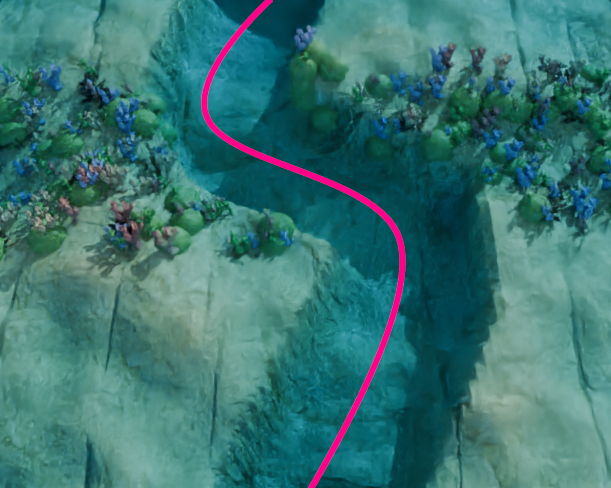
\includegraphics[width = 0.3 \linewidth]{Figures/Interactions/InteractionEdition1.png}
    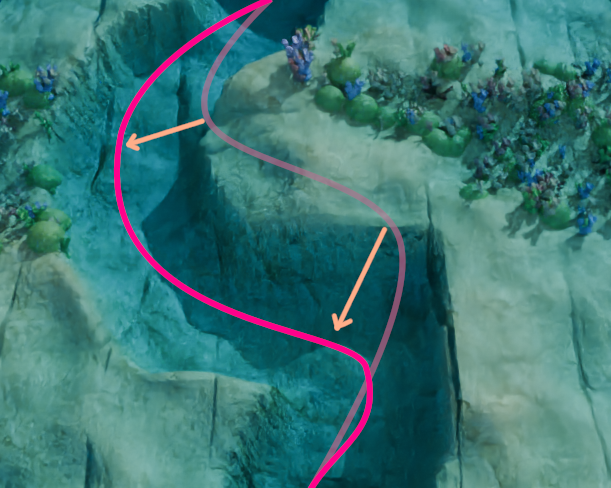
\includegraphics[width = 0.3 \linewidth]{Figures/Interactions/InteractionEdition2.png}
    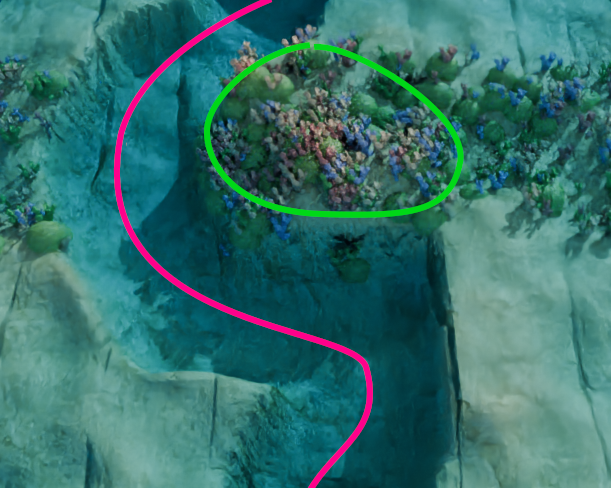
\includegraphics[width = 0.3 \linewidth]{Figures/Interactions/InteractionEdition3.png}
    \caption{Starting from a coral colony developed around a canyon (\textit{left}), the user edits the shape of the canyon, resulting in a different configuration of the scene, killing the corals that ends too deep in the water (\textit{center}) and the development and growth of new corals at the previous location of the canyon (\textit{right}). }
    \label{fig:semantic-representation_user-interaction}
\end{figure}

As long as a non-zero fitting function is defined in the terrain, new environmental objects can be forced by the user at any point of the simulation. 

% \subsubsection{Guiding the simulation}
Control over the region of the terrain that should be updated can be given by adjusting all fitting functions through a scalar field $\influence: \R^2 \to \R $ such that the fitting function $\fittingFuncObj(\p)$ of any new environmental object is evaluated as $\fittingFuncObj^*(\p) = \influence{\p} \fittingFuncObj(\p)$. This is especially useful in the planning of robotic simulations as we can first generate the overall shape of our terrain and secondly focus the generation process around the areas that may be visited by the robot, avoiding useless simulations and computer power. 
Figure~\ref{fig:semantic-representation_coral-colonization-scene} shows an example of colonization of the coral polyps that we limited manually into an annulus.
% Figure~\ref{fig:semantic-representation_focus-area-example} shows an example of colonization of the coral polyps that we limited manually.

% \begin{figure}
%     \centering
%     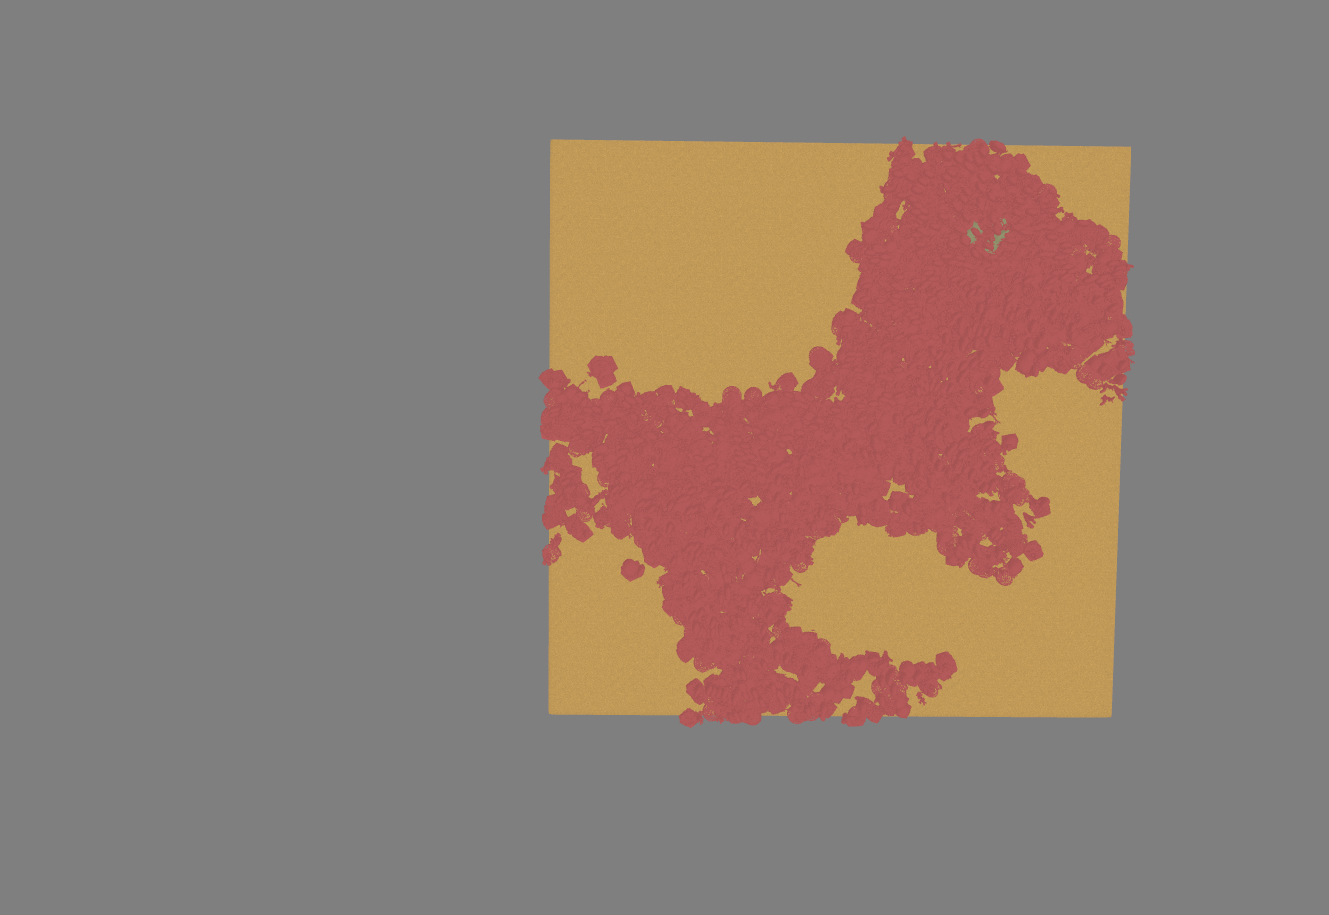
\includegraphics{Figures/UserControl/guidedGeneration1.png}
%     \caption{Controlling the generation area can produce a user-defined focused shape.}
%     \label{fig:semantic-representation_focus-area-example}
% \end{figure}

% - Changing the water currents \\
Our water current simulation is modeled as a simple vector field. As such, the user is able to interact with it at any moment of the simulation, allowing for the death of sensible environmental objects while it will guide the simulation into a new landscape. By modifying the water currents, the user also modifies the transport rate of materials at this position. The modification of currents is given as a stroke, a parametric curve $\curve$ for which we evaluate $\Delta \Wuser(\p)$ just as for curved environment objects (Section~\ref{sec:semantic-representation_water-currents}).

\subsubsection{Geological events}
\label{sec:semantic-representation_events}
A configuration file can define in advance the different events that should be triggered during the simulation. This can be useful to generate landscapes that are close to some existing locations. 
Multiple geological events can be triggered either as sudden or continuous environmental changes. These changes play a huge role in the morphology of landscapes.
We define events with a starting point and an ending point, such that at any time of the simulation we can compute the progress of the event as $\tEvent \in [0, 1]$.

Water level changes are important events that shape the underwater landscapes. As previously submerged environmental objects get elevated above water level, flora and fauna terrain elements dry and die. Deprived from the living part of the elements, everything is more affected by terrestrial erosion. By updating the value of the depth $\depth$ evaluated in the fitting functions, any environmental object that is sensible to the depth will be impacted automatically, that may be causing death (Figure~\ref{fig:semantic-representation_water-event}). The modification of the water level is defined as 
\begin{align*}
    \depth(\p) = \depth_0(\p) + \sum_{e \in \events} \Delta \depth_e \tEvent
\end{align*}
with $\Delta \depth_e$ the amount of water rising or lowering during an event. We assumed a linear evolution of the water level during an event. This allows to evaluate the depth at any point in space and in time.

\begin{figure}
    \centering
    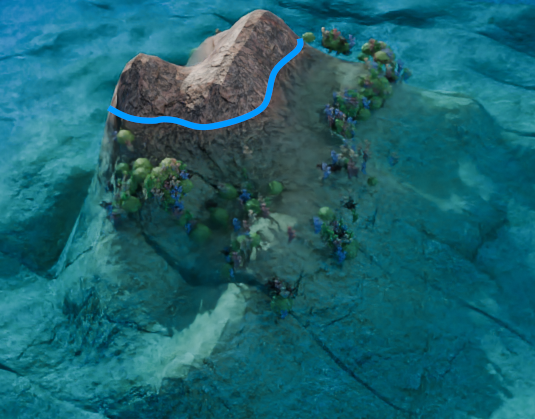
\includegraphics[width = 0.45 \linewidth]{Figures/Interactions/InteractionWater1.png}
    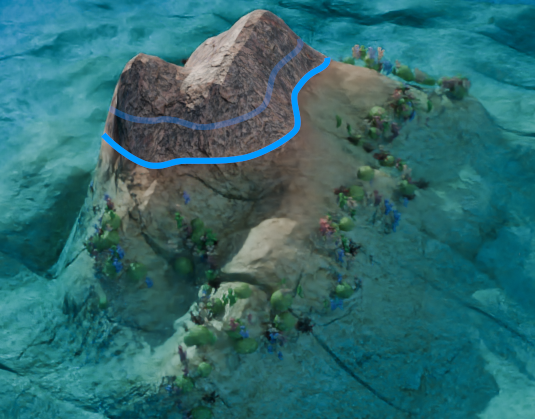
\includegraphics[width = 0.45 \linewidth]{Figures/Interactions/InteractionWater3.png}
    \caption{Lowering the water level by a few meters caused most of the coral objects to satisfy $\fittingFuncObj \leq 0$, causing their death. Since the water level (blue) decrease slowly, new coral objects spawn progressively at a lower altitude.}
    \label{fig:semantic-representation_water-event}
\end{figure}

Subsidence and uplift are the main geological events that create or destroy islands in the long term. These events are simulated as a simple factor on the height field of the generated terrain (Figure~\ref{fig:semantic-representation_subsidence-event}). Subsidence is not always uniform in the terrain. As such, the user can provide a position $\q$ at which the subsidence is the strongest, the amount of subsidence applied $\Delta \height_e$ and a standard deviation $\std$ for which we can then compute at any point in space and time of the simulation the height of the terrain
\begin{align*}
    \height(\p) = \height_0(\p) \cdot \sum_{e \in \events}{\frac{G(\norm{\p - \q})}{G(0)}} \Delta \height_e \tEvent 
\end{align*}
with $G(x)$ the Gaussian function
\begin{align*}
    G(x) = {\frac {1}{\std {\sqrt {2\pi }}}} \exp \left(-\frac {x^{2}}{2 \std ^{2}}\right)
\end{align*}

\begin{figure}
    \centering
    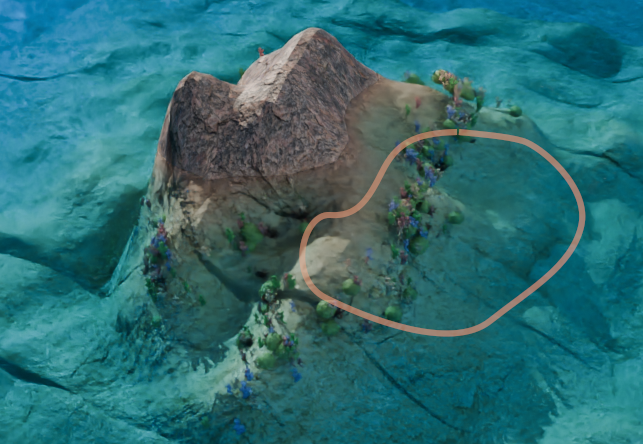
\includegraphics[width = 0.45 \linewidth]{Figures/Interactions/InteractionSubsidence1.png}
    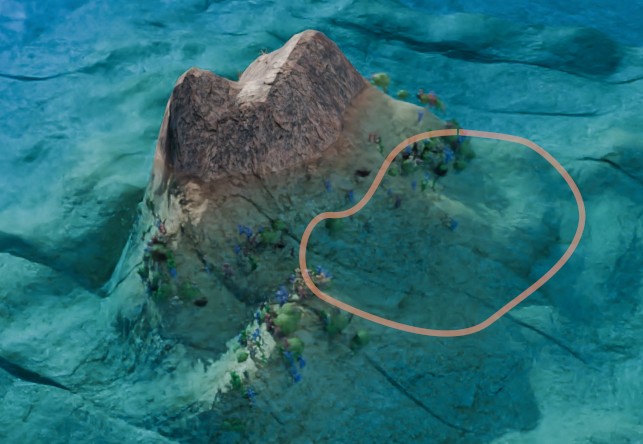
\includegraphics[width = 0.45 \linewidth]{Figures/Interactions/InteractionSubsidence2.png}
    \caption{Simulating subsidence on a part of the terrain (brown area) cause the depth value to change locally, resulting in the death of coral objects that find themselves too deep to survive. Here two subsidence events are triggered in parallel. }
    \label{fig:semantic-representation_subsidence-event}
\end{figure}

Storms are factors of the geomorphology of coral reefs \cite{VilaConcejo2016, Oron2023} and coasts \cite{Dominguez2005, Cowart2010}. Due to the extreme wind and wave velocities coasts are highly eroded in a short time period and the more fragile corals near the water surface are broken, possibly causing breaches in the reefs and spreading polyps in the currents direction. While there are many factors at play to understand the apparition of storms and the hydrodynamics affecting it, we simplified the model of storms to the user as a single epicenter $\q$ with a wind velocity $\windVelocity$ and a standard deviation $\std$ representing the spread around the epicenter (Figure~\ref{fig:semantic-representation_storm-event}). The computation of water currents are then computed as 
\begin{align*}
    \Wuser(\p) = \Wuser^*(\p) + \sum_{e \in \events | \tEvent \in [0, 1]} {\windVelocity \frac{G(\norm{\p - \q}}{G(0)}}
\end{align*}
In this case, we did not include the linear factor $\tEvent$ as storms are usually conserving a constant force for the time of the few weeks or months of their occurrence. 

\begin{figure}
    \centering
    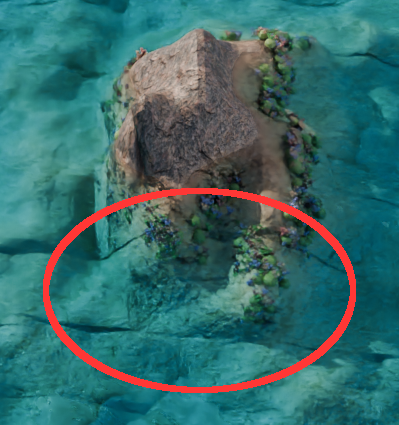
\includegraphics[width = 0.45 \linewidth]{Figures/Interactions/interactionStorm1.png}
    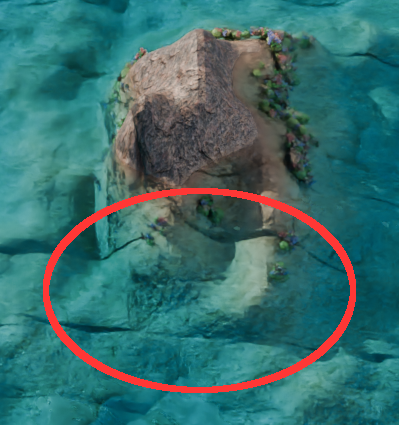
\includegraphics[width = 0.45 \linewidth]{Figures/Interactions/interactionStorm2.png}
    \caption{The result of a storm localized on one side of the island (red area) modifies the result of the evaluation of environmental objects around its epicenter for a short period of time. Most of the coral objects died from the event, except few environmental objects less sensible to water currents strength. }
    \label{fig:semantic-representation_storm-event}
\end{figure}

% Just as for the rise and lowering of water level, the heat is modeled as a simple value of the environment. For shallow areas (<100m) we assume a linear relation between depth and temperature, and a constant value for the terrestrial environment. As such, we can model a heat wave by a change of the environment values. Environmental objects who are sensible to temperature may die instantly. The modification of the temperature is defined as 
% \begin{align*}
%     \temperature(\p) = T_0(\p) + \sum_{e \in events} \Delta \temperature_e \tEvent + c \depth(\p)
% \end{align*}
with $\Delta \temperature_e$ the change of heat during an event, $\temperature_0$ the temperature at the water surface, and $c$ a very small factor.

The framework can easily be extended as the geological event system stays similar for all events. Including higher level simulations in the event system can be added, such as the simulation of tectonic activity, the use of fluid dynamics for tsunami events, the integration of human activity, ...

\section{Expert knowledge integration}
\label{sec:semantic-representation_biology}
  The definition of the fitting functions of the environmental objects are inspired by the biological and geological factors that rule the evolution of underwater landscapes. The main factors are depth, light, water currents and biodiversity. External events have direct and indirect repercussions on the biodiversity of underwater environments. Coral islands are complex bio systems in which fauna, flora and geology are mixed together. 

\subsection{Environmental objects description}
\label{sec:semantic-representation_represented-objects}
We have represented with environmental objects some geologic elements, animal elements and flora elements. The low island is most often raised in a circular shape as the process mainly appear around a hot spot under the ground. The evolution of an island into a coral island requires that the environmental conditions are sufficient for coral development: corals will grow slightly below the water surface as waves will break its growth and at a shallow depth (around 3m to 30m deep) in order for light to reach it. As coral grow and die, the skeleton is transformed into porous limestone, providing shelter to surrounding animals and reducing the impact of water erosion on the island. Corals drop polyps that are transported by the water flow and when they stick to a hard surface, as a rock or the reef itself, the coral may grow and colonize the area. As subsidence cause the island to lower, the living part of the coral reef keep growing toward light, which lead to a reef that is constantly close to the water level without reaching it due to wave erosion. The survival of reefs depends on the equilibrium between coral growth and and erosion. Eroded parts of the reef falling in the sheltered part of the reef accumulates, ending up by forming a lagoon. An island formed by a hot spot will inevitably subside in time, until it is completely flatten. As the coral reefs keep growing, only the lagoon remain, resulting in an atoll. \\
In this work we we integrate the biological and geological knowledge in the fitting functions of the environmental objects we want to generate. We represent the islands as regions that can be appearing with a uniform distribution. From the formulation of the region description \eqref{eq:internal-energy-equation}, we mostly create circular islands. The coral elements, environmental objects described as a single point, have a fitting function that take into account the depth of the ground, the amount of sand, fresh water and polyps in their environment, as well as the strength of water currents. Each coral species have different living conditions, but we reduced our work to soft coral which are sensible to water strength and stony corals that are more resistant to erosion. Reefs are formed as coral's skeleton are transformed into calcareous stone, describing then as an environmental object representing multiple others. 

\subsection{Simplifications}
\label{sec:semantic-representation_simplifications}
The environmental factors simulated are greatly simplified as the real processes are in a very small time scale, that computer simulation are not able to simulate in interactive time. The use of environmental objects aim to represent a plausible results, while avoiding modeling the smaller scale events. Examples of simplifications are the geometry and material of each environmental object, which have an influence on the water currents through friction, the water currents represented as stationary flows, while the water flow dynamics are a complex system that may change completely at two different times of the day, the animal influence on the reefs that they transform by the ingestion and deposition of sediments, ...


\section{Results}
\label{sec:semantic-representation_results}
Our method provides a way to generate scenes at different scales. We demonstrate this capacity with the generation of a large scene of an island (Figure~\ref{fig:semantic-representation_teaser}) after what we focused the generation process in a canyon (Figure~\ref{fig:semantic-representation_canyon-scene}), then a small-scale visualization of coral colonies (Figure~\ref{fig:semantic-representation_coral-colonization-scene}).
In the examples, we rendered the environmental objects as a implicit tree or as individual meshes. The island, lagoons, reefs, canyons and sand ripples as implicit surfaces

% \subsection{Mid-scale}
% \label{sec:semantic-representation_mid-scale}
A canyon scene can be generated using our method. The water flow is affected by the curve of the canyon such that the currents are oriented in the direction of the curve's tangent.In this example, we force the position of arches to be inside the canyon. The arches deposits a material "rock deposit", which is the main element of the fitting function of the Rock object. The "rock deposit" is slightly affected by water currents, but its mass make it highly affected by gravity. As such, rocks will spawn underneath arches. In reality, an arch is often created as part of a large coral boulder that sees the calcareous bottom part detached by the water currents, often resulting in an arch surrounded by big rocks and smaller rocks from the erosion of the first rocks.
As such, we define an environmental object "Arch" with a fitting function $\fittingFunc_{arch}(\p) = 5 - d(canyon - \p) * \norm{\Water(\p)}$, an environmental object "Rock" using $\fittingFunc_{rock}(\p) = \material_{rock\_deposit}(\p)$ and Pebble using $\fittingFunc_{pebble}(\p) = \material_{smaller\_rock\_deposit}(\p)$. Finally, sand ripples are simply described as curves appearing where there is a lot of sand available: $\fittingFunc_{ripple}(\p) = \material_{sand}(\p)$.
Following these simple rules, Figure~\ref{fig:semantic-representation_canyon-scene} shows the emergence of details in the scene. 

% \subsection{Small-scale}
% \label{sec:semantic-representation_small-scale}
In this example we defined three different types of corals, coralA, coralB and coralC, to illustrate the possibility to model behaviours from the choice of fitting functions. Each of the coral types deposits a material "coral polyp" and "coral polyp A" ("coral polyp B" and "coral polyp C" respectively). By considering a fitting function that minimize the ratio $\frac{\text{coral polyp}}{\text{coral polyp A}}$, we can see an emergent behavior of the three types of coral fighting for the space colonization.
Figure~\ref{fig:semantic-representation_coral-colonization-scene} shows the result of this simulation at three different interations. At the border between two colonies, none of the colonies make progression due to the amount of coral polyp specific from the other colony.

\begin{figure*}
    \centering
    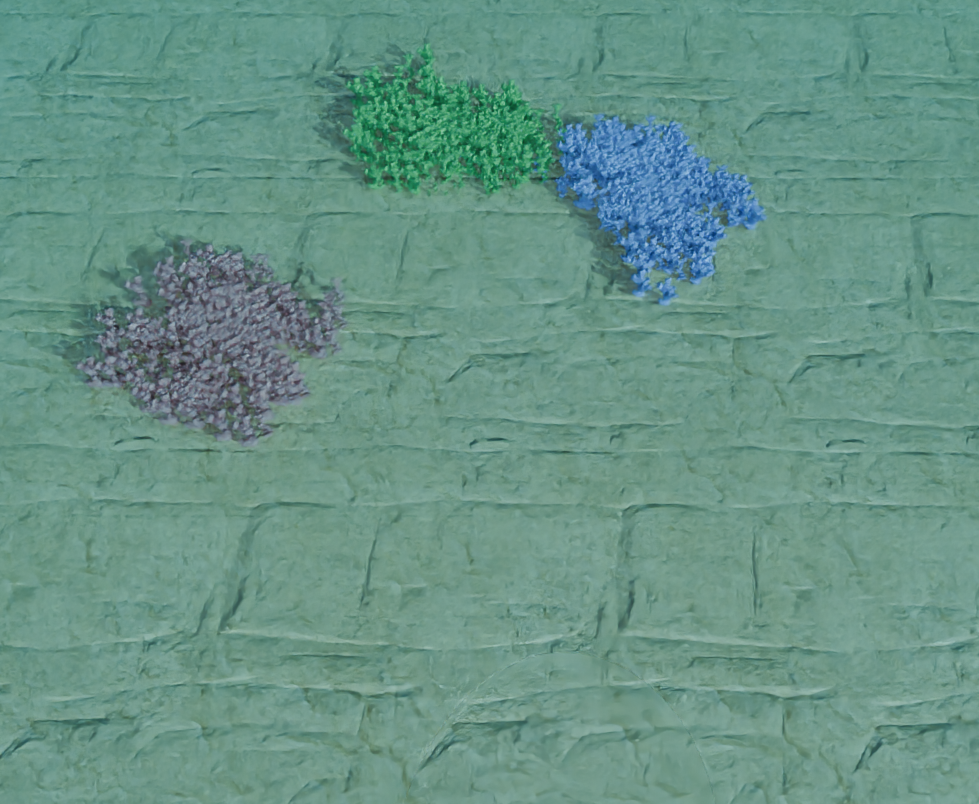
\includegraphics[width=0.245 \linewidth]{Figures/Colonization/col0.png}
    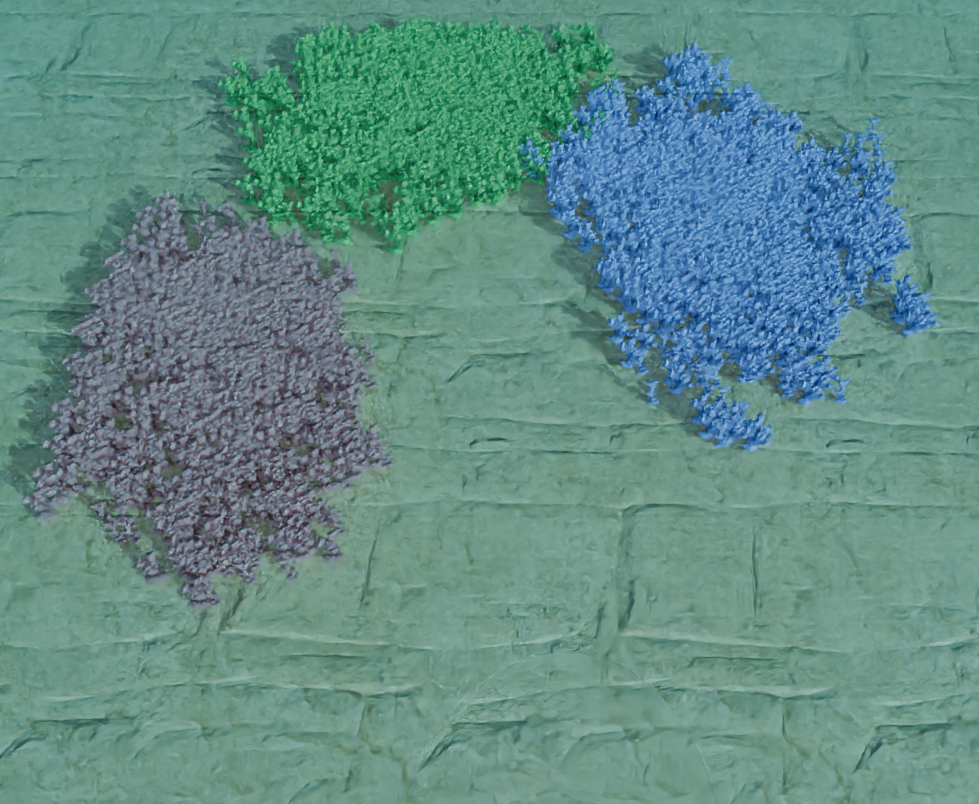
\includegraphics[width=0.245 \linewidth]{Figures/Colonization/col1.png}
    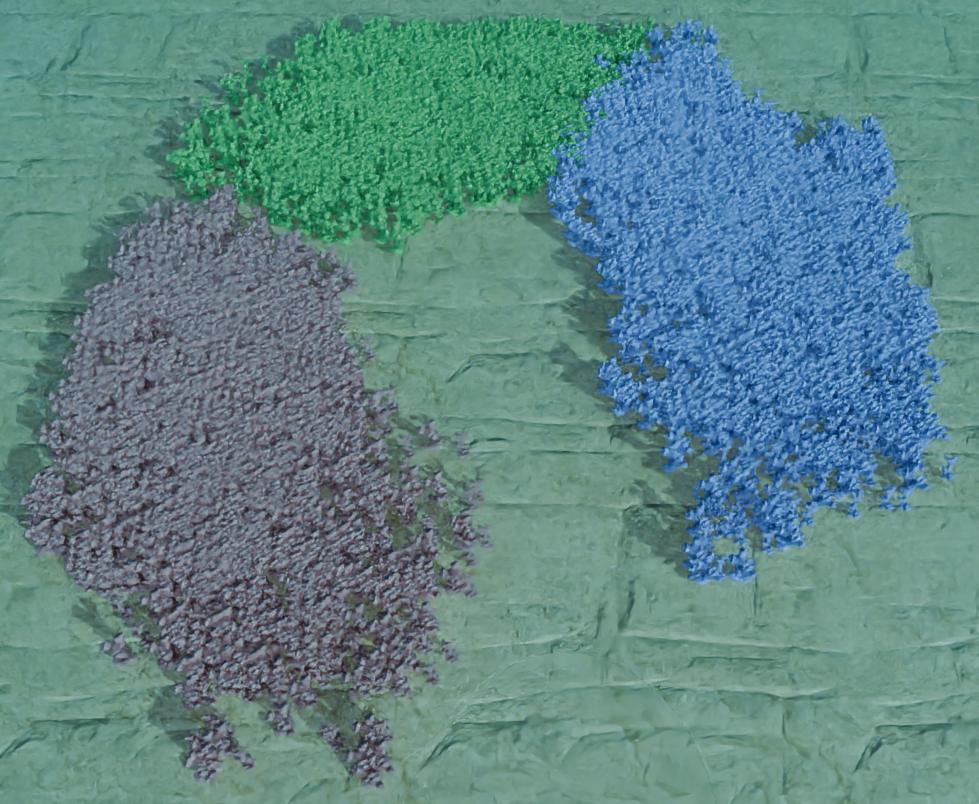
\includegraphics[width=0.245 \linewidth]{Figures/Colonization/col2.png}
    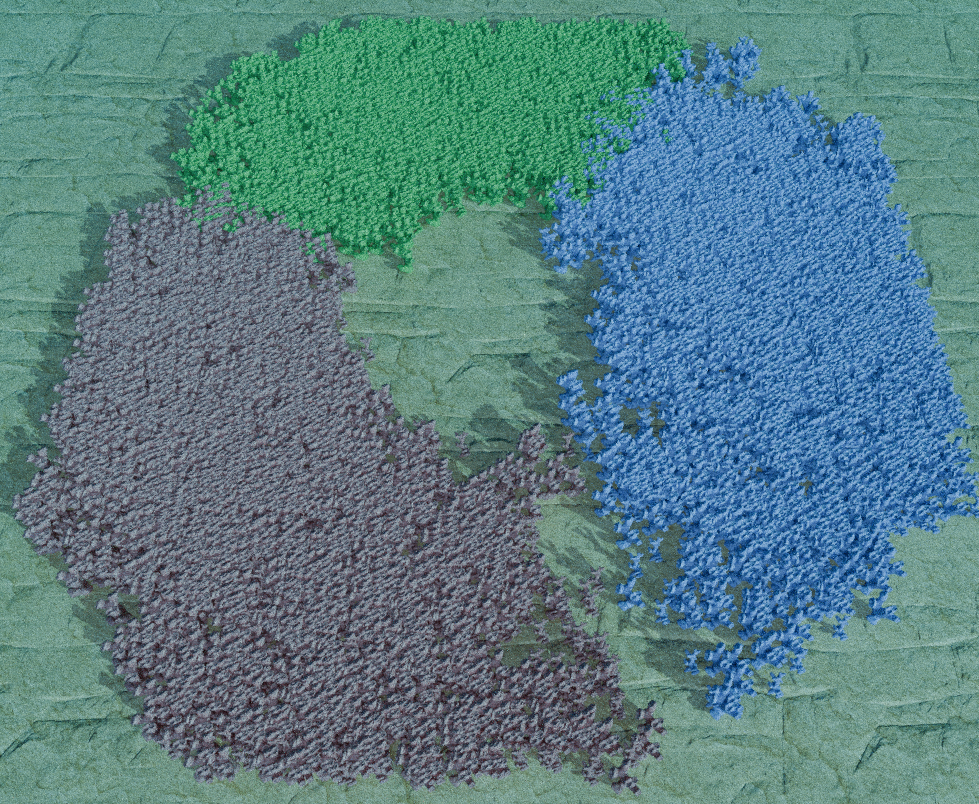
\includegraphics[width=0.245 \linewidth]{Figures/Colonization/col3.png}
    \caption{Three colonies of coral (red, blue, green) restricted to an annulus the middle section of the terrain fighting for the space.}
    \label{fig:semantic-representation_coral-colonization-scene}
\end{figure*}

\begin{figure*}
    \centering
    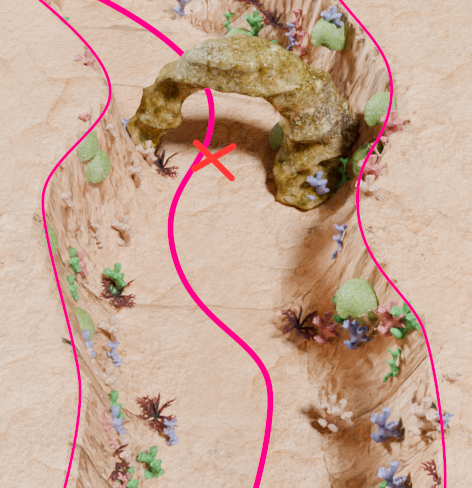
\includegraphics[width = 0.24 \linewidth]{Figures/Canyon/Canyon2.png}
    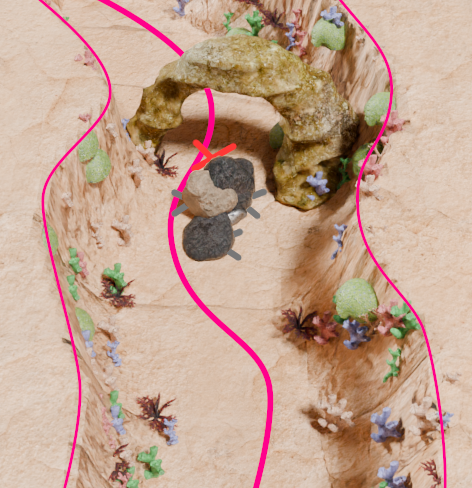
\includegraphics[width = 0.24 \linewidth]{Figures/Canyon/Canyon3.png}
    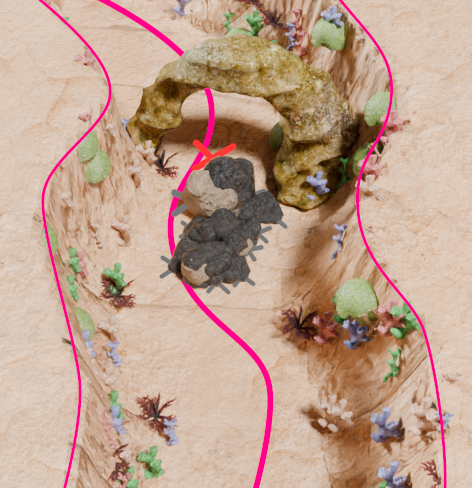
\includegraphics[width = 0.24 \linewidth]{Figures/Canyon/Canyon4.png}
    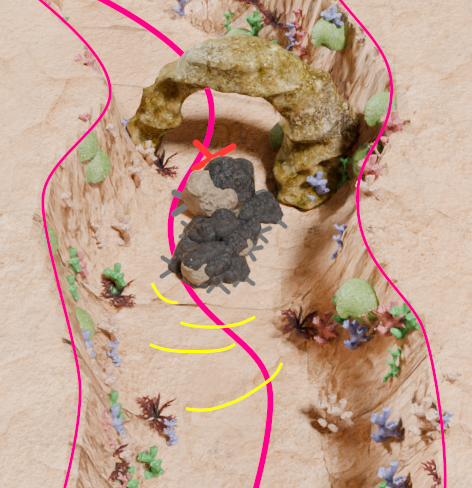
\includegraphics[width = 0.24 \linewidth]{Figures/Canyon/Canyon5.png}
    \caption{Evolution of a canyon scene at different iterations of the simulation. The apparition of an arch causes the spawning of rocks, pebbles, and finally some deposition of sand at the bottom of the canyon, spawning ripples. }
    \label{fig:semantic-representation_canyon-scene}
\end{figure*}



\section{Discussion}
\label{sec:semantic-representation_discussion}
The proposed method aims to generate plausible landscapes using simplified versions of the evolution of an ecosystem and of the 3D representation. The biological realism of the result is highly correlated to the amount of simplification and assumptions, while the visual realism is completely dependent to the geometric functions used for the 3D modeling of the environmental objects. While proposing a flexible method that propose a generic approach for terrain generation, a close collaboration with fields experts and with graphists is needed to achieve optimal results.

Most simulation algorithm's quality depends on the size of the time step used, but with the introduction of a decay rate in the materials properties, we limit the influence of time steps by considering that steady-state are reachable. The material deposition and absorption on punctual environmental objects can be seen as a Dirac function $\dirac$ centered at their position resulting in the advantage that material displacement function can use the definition of the diffusion equation instead of the advection-diffusion-reaction equation. This equation allowing us to evaluate the state of the material $\material$ without intermediate steps, but this is not applicable with curve- and region-based environmental objects. 

\section{Conclusion}
\label{sec:semantic-representation_conclusion}
We have proposed a method to generate terrains procedurally using sparse representations. This representation, the environmental objects, enables to introduce expert knowledge by the mean of the fitting functions that rule the environmental objects life cycle, but also to integrate the user in the loop during the generation process. We reduced the terrain resolution limitations by defining the environment objects as parametric elements. Thanks to the sparse representation based on single points, curves and regions, we allow for direct manipulation of the environmental objects of the scene by the user which, thanks to the environment steady state consideration, also enables to include these interactions in the automatic simulation process. \\
Integrating environmental properties in the fitting function of environmental objects allows the user to guide the generation through geological events. Our method enables each environmental object of the scene to influence the environment locally, reducing the need of computations while also retrieving environment values locally, which result in a parallelizable life-like simulation process. The genericity of the environment properties definitions should be sufficient for plausible generation of other landscape types as long as expert knowledge can be translated to environmental object's formalism.


We limited our work to the use of 2D scalar fields as they are more easily differentiable, interpretable and lighter than volumetric representations. However, future works include using 3D representations of the terrain and the environment to generate 3D terrains, including cavities, sub-terrestrial areas and the interior of coral structures. 
% The different possibilities to explore for this would be: the use of 3D particles to represent the state of the materials in the environment, or voxel grids or flatten representation of the terrain's surface (but would not allow a different morphological shape than the height field...).

\def\url#1{} % This line actually remove the "URL" link from the references


\begin{figure*}
    \centering
    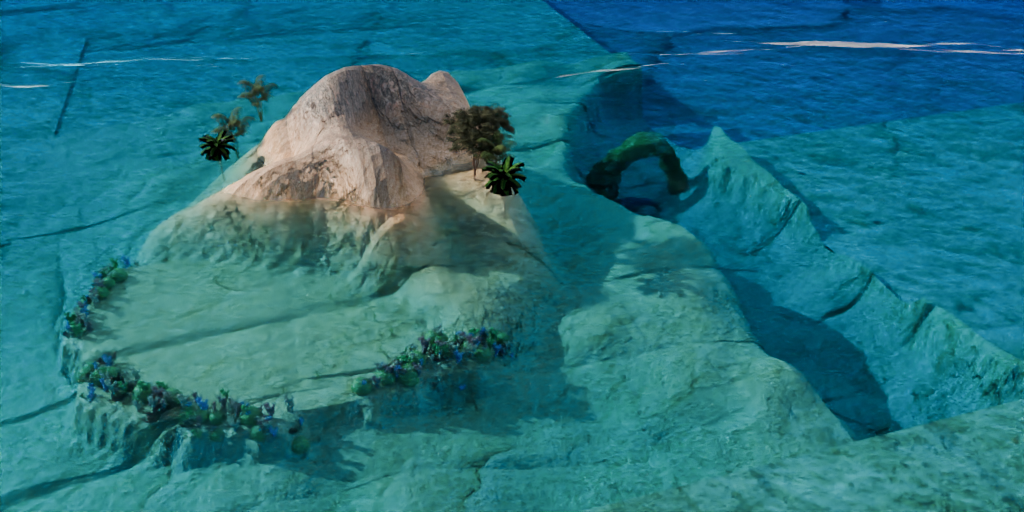
\includegraphics{Figures/CoralIsland/multiScene1 v2 final 1.png}
    \caption{A simple coral island is generated using an island, a lagoon, reefs coral polyps, beaches, trees and algae environmental objects. Trees appear on beaches and algae grow in the lagoon's sand. }
    \label{fig:semantic-representation_coral-island-scene}
\end{figure*}

% bibtex
%\bibliographystyle{eg-alpha-doi}
%\bibliography{references_terrain}

% biblatex with biber
% \printbibliography

%\end{document}
%
%- Qu'est-ce qu'une representation sémantique ? \\
%** Définition linguistique + Définition image + notre définition \\
%- Pourquoi une representation semantique? \\
%** Partage de connaissances avec biologistes, geologues, etc... \\
%** Données de carnets de voyages, cartes labellisées, ... \\
%- Avantages et inconvéniants de la representation sémantique \\
%** Avantages: \\
%*** Interpretation \\
%*** Control utilisateur \\
%*** Abstraction representation 3D \\
%** Inconvéniants: \\
%*** Besoin de connaissances experts (+ problèmes communication interdisciplinaire) \\
%*** Simplifications nécessaires sur la physique / phénomènes naturels \\
%- Representation 3D des terrains semantiques \\
%** Mélanges de méthodes possibles (fonctions implicites + maillages)
%
%\section{Representation de terrain parsemée}
%- Paysage contient des structures de tailles très variables :\\
%** Montagnes sur plusieurs km² mais rivières larges de quelques mètres, par exemple \\
%- Proposition de representation du terrain de manière parsemée \\
%** Definition des éléments du terrain par un objet simple : objets environementaux \\
%** Géométrie implicite, proposant un affichage 2D ou 3D \\
%** Possibilité "facile" de LOD \\
%- Méthode de génération itérative de terrain parsemé \\
%** Reduire temps de calcul $O(n^2)$ à $O(n)$ par l'utilisation de l'environnement comme proxy\\
%** Méthode basée sur la déposition de matériaux \\
%** Processus stochastique itératif
%
%\section{Objets environnementaux}
%- Symbolique de l'objet environnemental \\
%- Reference "Environmental Objects" \\
%- Comparaison aux biotopes
%
%\subsubsection{Definition}
%- Squelette \\
%- Forme paramétrique \\
%- Conditions de vie
%
%\subsubsection{Implémentation}
%- Instantiation des objets \\
%** Definition du squelette \\
%*** Points, courbes, régions \\
%*** Utilisation Snake
%** Definition geométrie \\
%- Modifications sur environnement \\
%- ...
%
%% \chapter{Snake - Active Contour Model}

We want to symbolize a dead coral area as a \gloss{EnvObj} "reef." To do this, the coral objects continuously deposit a quantity of "dead coral" material. This material, stored in a discrete scalar field, contains high intensities where a reef should supposedly exist. 
We need to draw a curve to represent this new object. The constraints of this curve are that it must pass through the points of highest intensity while maintaining a given length.

The Snake algorithm, or Active Contour Model, approaches this application. The algorithm proposes to give an energy to the curve, which then tries to minimize it through gradient descent.

The energy, in the initial paper, is defined by
\begin{align}
    \Esnake^{*} = \int \limits _{0}^{1} { \Esnake(\mathbf {v} (s))\,ds } = \int \limits _{0}^{1} { \Einternal (\mathbf {v} (s)) + \Eexternal (\mathbf {v} (s)) } \,ds
\end{align}

The internal energy represents the properties of the curve while the external energy represents properties of the field it lies in. In the original paper they are described as: 
\begin{align}
    \Einternal &= \alpha \Econt + \beta \Ecurv \\
    \Eexternal &= \gamma \Eimage
\end{align}

The continuity cost $\Econt$, originally defined as the minimization of the spacing between the points $\left\|{\frac {d{\bar {v}}}{ds}}(s)\right\| ^{2}$, does not make much sense in the discrete form of the algorithm. In its discrete form, we seek to maintain a regular interval between the points by applying $\Econt = \left(\tilde{d} - \left\|p_i - p_{i-1} \right\| \right)^2$ with $\tilde{d}$ being the average distance between each point.

The curvature cost $\Ecurv$ seeks to minimize the oscillations of the curve and can thus be defined as the squared second derivative $\left\|{\frac {d^{2}{\bar {v}}}{ds^{2}}}(s)\right\| ^{2}$.

The discrete form $\Ecurv^{*} = \left\| p_{i-1} - 2 p_i + p_{i+1} \right\| ^2$ is not necessary with splines, due to their closed form.

The image cost $\Eimage$ tries to attract the points of the curve to a local maximum of the image gradient. It is defined as $\Eimage = - \left\| \nabla I \right\| $.

We want to see our curve maintain a given length $L$. We then modify the formulation of the continuity cost to become $\Econt = \left(\tilde{l} - \left\|p_i - p_{p-1} \right\| \right)^2$ with $l = \frac{L}{n - 1}$, knowing $n$ is the number of vertices of the curve. Additionally, we want a curve that follows points of high intensity rather than the gradient, which leads to modifying the image cost $\Eimage = -I$.

The calculation of the gradient $\nabla \Esnake$ remains trivial in parts:
\begin{align}
    \frac{\partial \Eimage}{\partial p_i} &= - \nabla I(p_i) \\
    \frac{\partial \Ecurv^{*}}{\partial p_i} &= -\frac{2 \left( p_{i-1} - 2 p_i + p_{i+1} \right) }{ \left\| p_{i-1} - 2 p_i + p_{i+1} \right\| } \\
    \frac{\partial \Econt^{*}}{\partial p_i} &= 2 \left(l - \left\|p_i - p_{i-1} \right\| \right) \cdot \frac{p_i - p_{i-1}}{ \left\| p_i - p_{i-1} \right\| }
\end{align}

We then have
\begin{align}
    \Esnake &= \alpha \left(l - \left\|p_i - p_{i-1} \right\| \right)^2 + \beta \left\| p_{i-1} - 2 p_i + p_{i+1} \right\| ^2 - \gamma I \\
    \nabla \Esnake &= 2 \alpha \left(l - \left\|p_i - p_{i-1} \right\| \right) \cdot \frac{p_i - p_{i-1}}{ \left\| p_i - p_{i-1} \right\| } - \beta \frac{2 \left( p_{i-1} - 2 p_i + p_{i+1} \right) }{ \left\| p_{i-1} - 2 p_i + p_{i+1} \right\| } - \gamma \nabla I(p_i)
\end{align}

It should be noted that the calculation of $\Econt^{*}$ uses the distance $\left\|p_i - p_{i - 1} \right\|$. For $i = 0$, the distance $\left\| p_i - p_{i + 1} \right\|$ is used.

If all the points of the curve are at a distance greater than $l$, the optimization will push each of these points to get closer to its predecessor. Point $p_0$, itself, will move very little, so the entire curve aligns towards point $p_0$. By using the distance to the successor $\left\| p_i - p_{i+1} \right\|$, the curve moves towards point $p_N$.
It is then possible to converge towards the median point by alternating the use of the distance with the predecessor and with the successor, at the cost of slower convergence.

The active contour model algorithm is highly sensitive to the initial curve placement. In cases where a portion of the curve is in an area with a very low gradient on $\Eimage$, the vertices of the curve will simply optimize $\Einternal$, resulting in a straight segment in a low-intensity area, while the rest of the curve optimizes correctly.

To mitigate this problem, we propose adapting the Snake algorithm into Caterpillar: throughout the gradient descent, the target length $L$ is artificially reduced and then increased. In this way, a portion of the curve blocked in a region without possible optimization on external energy will be attracted by the optimized curve until it falls on a strong gradient. The dead portion can take the place of optimized vertices. By returning the target length $L$ to its initial value, the optimization continues with fewer vertices in the dead zone. Repeating this process gradually brings all points into an optimizable area. However, a too-rapid change in the target length can prevent the vertices from optimizing $\Eexternal$ by amplifying $\Einternal$ too much. Additionally, this algorithm can lead to numerical errors and slower convergence.

%
%
%\subsection{Communication entre objets}
%- Comparaisons avec réalité \\
%** Pas de communication directs entre les éléments \\
%- ...
%
%\subsubsection{Échanges par l'environnement}
%- Modifications de l'environnement \\
%** Absorption \\
%** Deposition \\
%** Modification des courants \\
%- Impact de l'environnement sur les objets \\
%- ...
%
%\subsubsection{Cycle de vie des objets environnementaux}
%- ...
%
%\section{Résulats}
%- ...


%\subsection{Outils implémentés}
%- Parseur de fonctions de coût \\
%- ...

%\section{Autre tentative}
%\subsection{Échanges directs}
%\subsubsection{Génération de graphe}
%\subsubsection{Triangulation de Delaunay}


%
%\section{Érosion continue}
%[POSSIBLEMENT À DEPLACER DANS EROSION] \\
%- ...
%
%\subsection{Description du problème}
%- Processus d'érosion est un système dynamique \\
%- Nombre de variables très important \\
%- Impossible de simuler à des pas de temps différents et/ou à différentes échelles/résolutions
%
%\subsection{Solutions proposées}
%- ...
%
%\subsubsection{Cycle de vie des objets environnementaux}
%- ...
%
%\subsubsection{Utilisation d'apprentissage profond}
%- ...




%\chapter{Influence sur la génération}
\minitoc


\section{Introduction}
This document aims to formalize a terrain generation method developed during my thesis.

The main issue this method seeks to address is the difficulty for a user to describe the environments they want to generate. By proposing a hierarchical structure in the description of elements to define, the environments exhibit adaptive representation granularity, catering both to the user's needs and hardware capabilities.

The key element of the method is the "biotope," defined as "a habitat defined by relatively uniform physical and chemical characteristics." (Source: Wikipedia)

In this context, we define the characteristics of a geographical region as well as the sub-biomes included within it.

Although this method was conceived with the aim of generating underwater environments, many examples given in this document will use elements present in surface environments, purely for simplification purposes.

\section{Glossary}
Initially, this document will present definitions of various terms used in the description of the method. By doing so, we hope to eliminate any ambiguity in the upcoming explanations. Definitions may appear in certain sections of this document if deemed too specific.

\textbf{Biotope}: The main element of the method used. The biotope (or, as I might often write, the biome) is a geographical region defined by topographic and geomorphological characteristics. The notion of biotope used does not distinguish between different scales (the biosphere and the ecosystem of a rock are represented uniformly), nor does it distinguish between living and mineral elements. The biotope is represented in two different ways in the terrain generation process: the model and the instance.

\textbf{Model (of biotope)}: The model (or biotope model, if the context requires) is a biological description of the geographical area. It remains an abstract, or literary, form of the biotope. It is defined by a list of characteristics related to topography (description of the relief, description of the shape of the region) and geology (type of soil, for example). One can also list the sub-biomes that compose it, specifying the quantity, proportion, chances of appearance, etc., of each sub-biome. This form is the user input into the system, but during the terrain generation process, the model's role is to create instances of itself to concretize the structure to be generated. In the document illustrations, if a model is represented in a graph, it will be symbolized by its name in quotation marks (e.g., "Forest," "Lagoon").

\textbf{Instance (of biotope)}: The instance is the concrete form of the model. Unlike the model, the instance takes place in space with fixed characteristics (unlike the probabilistic characteristics of the model). Through generation rules and living conditions defined by the user and the system, the biotope instance has a geometric shape and neighboring relationships with other instances. An instance, like its original model, consists of sub-biomes. The instance remains linked to its original model. To distinguish the instance from the model in the document illustrations, if represented in a graph, the instance will be symbolized by the model's name followed by a hash and an instance number (e.g., Forest \#1, Lagoon \#28).

\textbf{Generation Rule}: Generation rules represent a list of obligations or prohibitions, including living conditions and adjacency rules.

\textbf{Living Condition}: In our definition, a biotope can only exist under certain environmental conditions in a specific place. The conditions can be multiple and will be listed in a subsequent chapter of this document. Vegetative elements, for example, have strong constraints in terms of sunlight exposure, the "snow" biotope requires a low temperature condition, and some biotopes like sand cannot exist on steep terrain. Living conditions are therefore important properties to express in biotope models. These conditions can be expressed probabilistically.

\textbf{Adjacency Rules}: Adjacency rules define how biotope instances can be arranged. There are three types of rules to express adjacency between two biotopes: prohibition, possibility, and obligation. Two models linked by an adjacency prohibition cannot generate instances with a common border. Conversely, a model linked to another by an obligation constraint can only generate an instance if it shares a border with an instance of the linked model. The possibility constraint is the default, where the instance is indifferent to the presence or absence of a common border. It is conceivable that the notion of "possibility" could be associated with a probability in the future, allowing for example, a lake to often be adjacent to an urban area, but an urban area to rarely be near a desert. For now, adjacency rules are bilateral: a rule that applies from biotope A to biotope B also applies from B to A. In the rest of the document, adjacency rules will mainly be represented by graphs (undirected) with the nodes as the models to be generated, solid edges representing the possibility of adjacency, dotted edges symbolizing an adjacency obligation (rarely used), and the lack of an edge indicating an adjacency prohibition.

\textbf{Adjacency Graph}: The adjacency graph, although similar to the representation of adjacency rules, this time represents the concrete topological adjacency between the generated instances (not the models). The adjacency graph consists of nodes representing each instance generated by the models and the edges representing the existence of a common border. Edges can only be present if the two biotope instances see their model linked either by an obligation or possibility of adjacency constraint. By definition, this graph must be planar. In this document, adjacency graphs will therefore be represented by graphs where the nodes are biotope instances (following the instance graphic convention), and an edge represents a topological adjacency.

\textbf{Region (of biotope)}: The region is the space occupied in a geometric sense by a biotope instance once represented in space. Among the important properties, one can note that a region has a shape and an area.

\textbf{Boundaries}: The boundary is the geometric adjacency of two regions representing biotope instances.

\textbf{Adjacent Regions}: Two regions are adjacent if they share a common edge. In a successful generation, a region shares a common boundary with regions represented by instances linked to the current region instance in the adjacency graph. We can then distinguish three types of connections between instances: correctly adjacent instances are linked in the adjacency graph and are adjacent regions, over-adjacent instances are not linked in the adjacency graph and are adjacent regions, and under-adjacent instances are linked in the adjacency graph and are not adjacent regions. The latter two types are maladjacencies.

\textbf{Biotope Characteristics}: Biotopes possess characteristics common at all scales, whether they represent geological or biological elements. The characteristics are defined in the models in probabilistic forms. Instances inherit a unique and fixed value for each characteristic from the original model. The characteristics notably define the shape the generated region will take, the relief, etc.

\textbf{Sub-biotope}: Each biotope can include one or more sub-biomes. This is how an environment can be defined on the scale of a planet as well as on the scale of a rock. The biotope specifies the number of instances to generate for each sub-biome, or the proportion of the surface to cover. The parent biotope provides an approximate description of its environment, but with each sub-biome, the description is refined.

\textbf{Recursive Tree}: The proposed method has a strong recursive nature through its representation in biotopes and sub-biomes. The biotope construction tree is thus a recursive tree of biotopes composed at the root of a biotope to be generated and whose nodes (and leaves) represent sub-biomes. The parent-child relationship defines the inclusion of the child among the sub-biomes of the parent node. The tree describing a biotope can then be reused to describe a larger biotope, up to a planetary scale or larger.

\textbf{User Action}: The user plays an important role in the terrain generation process. By user action, we mean any action performed during the process. User actions are applied to biotope instances: adding, replacing, or deleting an instance, or modifying the characteristics and living conditions of an instance.

\textbf{Primitives}: Primitives are simple geometric representations that can be combined to represent more complex structures. Among these, we can notably find: the point, the curve, the sphere, and the 3D model.

\section{Environment description}
In this method, an environment is defined by a biotope model for which characteristics such as the general shape of its region, the biotope's relief, or the representative primitive of the biotope are specified, as well as living conditions such as altitude, temperature, and necessary luminosity for its survival. These characteristics are uniform across the entire biotope region; the only way to vary them is to add sub-biomes in the definition, which will take the form of sub-regions of the parent. Sub-biomes have the same types of characteristics and living conditions, which they can define in their own way, as well as their own sub-biomes.

Thus, the environment description is carried out recursively until the level of detail is sufficient for the modeler.

A biotope model can be the sub-biome of several different biotope models, offering the possibility to define complex environments quickly.

\subsection{Biotope characteristics}
The biotope model allows the user to describe the biotope's appearance to be generated. This description is probabilistic, and instances derived from the model each define a unique value for each characteristic respecting the probability law described by the model. The list of characteristics includes:
\begin{itemize}
	\item Region size: This represents the area of the surface (without considering relief) that the region occupies in space.
	\item Altitude (min and max): These two characteristics represent the altitudes the biotope can reach.
	\item Relief (frequency and amplitude): These characteristics describe the terrain's gradient. High relief amplitude symbolizes significant disturbances on the ground, unlike low amplitude, which
	
	indicates the ground is relatively flat.
	\item Primitive (type, dimension, position): The primitive determines the basic element represented by the biotope.
	\item Shape: The biotope region's shape in space.
\end{itemize}

To facilitate the user's work, default values are proposed for each biotope, respecting each type of primitive.

\subsection{Living conditions}
The living conditions of a biotope define the specific properties necessary for the biotope to survive. To be viable, the biotope must respect these conditions. These properties may relate to the following conditions:
\begin{itemize}
	\item Luminosity (min and max)
	\item Temperature (min and max)
	\item Soil type
	\item Exposure (direction, minimum and maximum angle)
\end{itemize}

Like characteristics, default living conditions are proposed to the user.

\subsection{Adjacency rules}
Three types of rules express adjacency between two biotopes: prohibition, possibility, and obligation. These rules define how biotope instances can be arranged spatially.

\begin{itemize}
	\item Prohibition: Two models linked by an adjacency prohibition cannot generate instances with a common border.
	\item Possibility: Instances can be adjacent, but it is not required.
	\item Obligation: Instances must share a common border.
\end{itemize}

\section{Generation process}
The terrain generation process involves creating instances from biotope models while respecting their characteristics, living conditions, and adjacency rules. This section details the steps of the process.

\subsection{Instance creation}
Each biotope model creates instances with fixed values for each characteristic derived from the probabilistic descriptions in the model. These instances are then positioned in space according to their characteristics and living conditions.

\subsection{Placement and adjustment}
Instances are placed in the environment, respecting their adjacency rules. If instances violate adjacency constraints, adjustments are made to either reposition instances or modify their characteristics within acceptable limits.

\subsection{User interaction}
Users can intervene in the generation process by adding, replacing, or deleting instances, as well as modifying instance characteristics and living conditions. These actions allow for fine-tuning the generated environment.

\subsection{Validation and refinement}
The final step involves validating the generated environment by checking for over- or under-adjacencies and making necessary refinements to ensure all instances adhere to their constraints and living conditions.

\section{Conclusion}
This method provides a structured approach to terrain generation by leveraging biotopes and their hierarchical organization. By defining biotopes probabilistically and respecting adjacency rules and living conditions, it is possible to generate diverse and realistic environments with varying levels of detail.

Future work may include refining probabilistic models for characteristics and adjacency rules, as well as exploring the use of probabilistic adjacency possibilities to further enhance the flexibility and realism of generated terrains.
%- ...
%
%\section{Génération de biotopes}
%- ...
%
%\subsection{Définition}
%- ...
%
%\subsubsection{Récursivité}
%- ...
%
%\subsubsection{Diagramme de Voronoï}
%- ...
%
%\subsubsection{Communication entre biotopes}
%- ...
%


\part{Modelisation}

\chapter{Modélisation de terrains volumiques [PEUT ETRE A DEPLACER DANS INTO]}
\minitoc

- Volumique est important pour représenter les structures en 3D \\
- Permet de representer des cavités, des arches, des superpositions, ... \\
- Notion de matériaux permet d'inclure beaucoup plus d'informations pour les parties suivantes : amplification et rendu \\
** Amplification (eg. érosion) doit connaitre le type de sol à la surface et sous-terrain pour être réaliste \\
** Rendu doit connaitre le matériau à la surface pour afficher correctement des textures \\
- ...


\section{Terrains implicites avec matériaux}
- ...

\subsection{Densité de matière}
- ...

\subsubsection{Granularité de matériaux}
- ...

\subsubsection{Soil triangle}
- ...

\subsection{Fonctions scalaires}
- ...

\subsection{Fonctions de mélange}
- ...

\subsection{Fonctions de placement}
- ...

\subsection{Utilisation de matériaux}
- ...

\subsubsection{Définition du matériau final}
- ...

\subsubsection{Post-processing : transformation de matériaux}
- ...



\section{Représentation graphique des objets environnementaux}
- Surfaces implicites \\
- Maillages \\
- ...


\chapter{Génération automatique d'îles coralliennes}
\label{chap:coral-island}
\minitoc

\section{Introduction}
\label{sec:coral-island_introduction}
- Definition ile corallienne \\
** Différents types d'iles coralliennes \\
*** Ici, iles volcaniques \\
- Presentation coraux \\
- Difference paysages normaux \\
** Notion de coraux \\
*** Evolution longue (ile) et courte (coraux) \\
**** Processus geologique affaissement de l'ile \\
- ...

\subsection{Théorie darwinienne}
- Plusieurs théories \\
- Impossibilité d'étudier aisément les environnements \\
** Utilisation d'observations \\
- Théorie réfutée par \cite{Droxler2021} \\
** Mais trop tôt pour juger \\
** Pratique dans notre cas. \\
- ...

\subsubsection{Multiples théories}
- Préciser autres théories : \\
** "Growth on Submarine Mountains Theory" (John Murray): Les récifs commencent sur les monts sous-marins et guyots, puis montent jusqu'à la surface petit à petit. \\
** "Sea Level Change Theory" (Reginald Daly) ["The Coral Reef Problem"] \cite{Daly1915}  : [A FOUILLER, JE L'AI PAS COMPRISE] \\
** "Erosion and Sedimentation Theory" (Maurice Ewing et William Donn) : [A FOUILLER] \\
** "Platform Reef Theory" (William Morris Davis) : [A FOUILLER] \\
- Les théories ne se contredisent pas forcement, elles peuvent être complémentaires pour expliquer des cas que d'autres n'expliquent pas. \\
- ...

\subsubsection{Voyage de Darwin}
- ...

\subsection{Overview}
- Outil proposé \\
** Sketching de l'île \\
** Sketching du profil \\
** Simulation de vents \\
- Automatisation des exemples \\
** Augmentation de données \\
- ...

\section{Related works}
\label{sec:coral-island_related-works}
- Perlin + falloff \\
** Mais manque de control \\
- Uplift [SCHOTT UPLIFT] \cite{Cordonnier2016,Cordonnier2017a} \\
** Mais proposons une méthode qui limite l'interaction demandée \\
- Sketching [PEYTAVIE SKETCHING, EMILIEN FIRST PERSON] \cite{Gain2009} \\
** Ajout de la contrainte radiale pour simplifier interaction \\
- Modelisation geologique \cite{Patel2021} \\
** Pour nous, pas facile à connaitre ce qui se passe sous terre (?) \\
- Contrairement à la litterature, integration de la partie sous-marine \\
** Integration de données d'observation dans notre processus \\
*** -> Forme type et profil type d'une ile \\
** Difficile d'intégrer des simulations physiques, car plutôt incertain \\
- Generation par couches permettrait d'améliorer le réalisme des exemples en considérant les interactions couches/environnement. \\
- ... 

\section{Génération d'exemples}
\label{sec:coral-island_example-generation}
- On utilise la théorie de Darwin dans notre cas car génération plutôt simple. \\
- 2 étapes: \\
** Génération de l'ile \\
** Génération du récif \\
- Nombreuses assumptions : \\
** Ile a une forme relativement ronde \\
** Corail pousse à une hauteur constante autour de l'ile \\
** Toutes "features" sont radiales \\
** Deformations des iles causées par les vents et vagues \\
** Les iles sont indépendantes les unes des autres \\
** Le profil est relativement identique tout autour de l'ile \\
- ... 

\subsubsection{Entrée}
- Sketching de l'ile vue de dessus + vue de profil \\
- Force des vents \\
- Niveau d'eau \\
- Taux d'affaissement \\
- ...

\subsubsection{"Simulation"}
- Affaissement calculé par simple scaling \\
** Attention aucune consistance geologique \\
*** Ici, utilisation d'un niveau zéro pour scale en Z \\
*** Pas de prise en compte des différents matériaux dans le sol \\
- ...

\subsubsection{Sortie}
- Height map de la surface de l'ile \\
- Zones d'ile et zones de corail \\
- Possibilité de recalculer la hauteur de sol et hauteur de corail \\
- ...

\section{cGAN}
\label{sec:coral-island_cGAN}
- ...

\subsection{Définition cGAN}
- ...

\subsection{Pourquoi un cGAN?}
- Flexibilité de l'entrée \\
- Sortir de la condition de l'entrée "radiale" \\
- Output même pour des données "incohérentes" (e.g. océan dans une ile) \\
- Pas de math, géométrie, géologie, ou choses compliquées à maitriser (hehe)

\subsection{Entraînement}
- ...

\subsubsection{Utilisation de données synthétiques}
+ Problème des données synthétiques \\
- ...

\subsubsection{Augmentation de données}
- ...

\subsection{Utilisation du modèle}
- ...

\subsubsection{Génération par sketch}
- ...

\subsubsection{Temps interactifs}
- ...

\subsubsection{Réalisme}
- ...



\chapter{Génération de réseaux karstiques}
\label{chap:karsts}
\minitoc

- ...

\section{Géologie}
\label{sec:karsts_geology}
- ...

\subsection{Formation}
- ...

\subsection{Intérêts}
- ...

\subsection{Place des karsts dans le projet}
- ...

\section{Contrôle utilisateur}
\label{sec:karsts_user-control}
- ...

\subsection{Méthode existante}
- ...

\section{Ma méthode}
- ...

\subsection{Karst en tant qu'arbre?}
- ...

\subsection{Génération de végétation -> Space colonization}
- ...




\part{Simulation d'érosion}

\graphicspath{ {./figures/} }

\chapter{Érosion par particules}
\label{chap:erosion}
\minitoc


\newcommand{\referenceExemple}[1] {\textit{Figure~\ref{tab:result_figures}: #1}}





\newcommand{\addingFiguresToCell}[4]{%
        \includegraphics[width=0.2\textwidth]{#1}
        \includegraphics[width=0.2\textwidth]{#2}
        \ifx\relax#3\relax
        \else
            \includegraphics[width=0.2\textwidth]{#3}
        \fi
        \ifx\relax#4\relax
        \else
            \includegraphics[width=0.2\textwidth]{#4}
        \fi
}

% The columns :
% Name & Results & Terrain representation & Dimensions & particles / iteration & iterations & particle radius & coefficient of restitution & particle density & capacity factor & erosion factor & deposition factor & Velocity field & computation time
\newcommand{\exampleCoastal}{
Coastal & \addingFiguresToCell{Results/Coastal_1.png}{Results/Coastal_2.png}{Results/Coastal_3.png}{} & \densityVox & 100x100x30 & 10 & 80 & 3 & 5 & 0.1 & 500 & 10.0 & 5.0 & 0.5 & Uniform & 0.5
}
\newcommand{\exampleGlacier}{
Glacier & \addingFiguresToCell{Results/Glacier1.png}{Results/Glacier2.png}{Results/Glacier3.png}{Results/Glacier4.png} & \heightmap & 100x100 & 20 & 80 & 3 & 10 & 0.1 & 500 & 1.0 & 1.0 & 1.0 & None & 0.8
}
\newcommand{\exampleLandslide}{
Landslide & \addingFiguresToCell{Results/Glacier_2_1.png}{Results/Glacier_2_2.png}{Results/Glacier_2_3.png}{Results/Glacier_2_4.png} & \heightmap & 100x100 & 20 & 200 & 10 & 2.5 & 0.2 & 500 & 0.1 & 1.0 & 1.0 & None & 4
}
\newcommand{\exampleHydraulic}{
Rain & \addingFiguresToCell{Results/Hydraulic1.png}{Results/Hydraulic3.png}{Results/Hydraulic5.png}{Results/Hydraulic7.png} & \heightmap & 100x100 & 20 & 100 & 10 & 1.0 & 1.0 & 1000 & 10.0 & 2.5 & 0.3 & None & 4.0
}
\newcommand{\exampleKarstBinary}{
Karst & \addingFiguresToCell{Results/KarstBinaryWithMarchingCubes1.png}{Results/KarstBinaryWithMarchingCubes2.png}{Results/KarstBinaryWithMarchingCubes3.png}{Results/KarstBinaryWithMarchingCubes5.png} & \binaryVox & 100x100x50 & 2 & 1000 & 40 & 5 & 0.5 & 500 & 10.0 & 5.0 & 0.5 & Uniform & 20
}
\newcommand{\exampleKarstBinaryStrata}{
Karst & \addingFiguresToCell{Results/KarstWithStrataNoise1.png}{Results/KarstWithStrataNoise2.png}{Results/KarstWithStrataNoise3.png}{Results/KarstWithStrataNoise4.png} & \binaryVox & 100x100x50 & 2 & 80 & 3 & 10 & 0.1 & 500 & 10.0 & 5.0 & 1.0 & Uniform & 0.8
}
\newcommand{\exampleLabyrinthOF}{
Glacier & \addingFiguresToCell{Results/LabyrinthOpenFOAM1.png}{Results/LabyrinthOpenFOAM2.png}{Results/LabyrinthOpenFOAM3.png}{Results/LabyrinthOpenFOAM4.png} & \densityVox & 100x100x40 & 2 & 80 & 3 & 10 & 0.1 & 500 & 1.0 & 1.0 & 1.0 & SIMPLE\cite{Caretto1973} & 0.8
}
\newcommand{\examplePipes}{
Tunnel & \addingFiguresToCell{Results/Pipes01.png}{Results/Pipes05.png}{Results/Pipes09.png}{Results/Pipes11.png} & \densityVox & 100x100x50 & 1 & 100 & 100 & 2.5 & 0.1 & 500 & 1.0 & 1.0 & 1.0 & None & 0.8
}
\newcommand{\exampleRiver}{
River & \addingFiguresToCell{Results/River1.png}{Results/River2.png}{Results/River3.png}{Results/River4.png} & \heightmap & 100x100 & 5 & 100 & 50 & 1.5-5 & 0.5 & 900 & 0.1 & 1.0 & 1.0 & None & 2.5
}
\newcommand{\exampleRiverTwo}{
River & \addingFiguresToCell{Results/River_2_1.png}{Results/River_2_2.png}{Results/River_2_3.png}{Results/River_2_4.png} & \heightmap & 100x100 & 5 & 100 & 50 & 1.5-5 & 0.5 & 900 & 0.1 & 1.0 & 1.0 & None & 2.5
}
\newcommand{\exampleRiverWater}{
\makecell{River\\(with water\\level)} & \addingFiguresToCell{Results/RiverWater1.png}{Results/RiverWater2.png}{Results/RiverWater3.png}{Results/RiverWater4.png} & \heightmap & 100x100 & 5 & 100 & 50 & 1.5-5 & 0.5 & 900 & 0.1 & 1.0 & 1.0 & None & 2.5
}
\newcommand{\exampleRiverObstacle}{
\makecell{River \\with obstacle} & \addingFiguresToCell{Results/RiverWithObstacle1.png}{Results/RiverWithObstacle2.png}{Results/RiverWithObstacle4.png}{Results/RiverWithObstacle6.png} & \heightmap & 100x100 & 5 & 100 & 50 & 1.5-5 & 0.5 & 900 & 0.1 & 1.0 & 1.0 & None & 2.5
}
\newcommand{\exampleWaterCurrents}{
Underwater & \addingFiguresToCell{Results/WaterCurrent1.png}{Results/WaterCurrent2.png}{Results/WaterCurrent4.png}{Results/WaterCurrent6.png} & \heightmap & 100x100 & 10 & 100 & 50 & 2.5 & 0.9 & 1000 & 1.0 & 1.0 & 1.0 & \cite{Stam2003} & 4
}
\newcommand{\exampleWindErosion}{
Wind & \addingFiguresToCell{Results/WindErosion1.png}{Results/WindErosion2.png}{Results/WindErosion4.png}{Results/WindErosion5.png} & \densityVox & 100x100x50 & 0.2 & 100 & 10 & 1.5 & 0.9 & 1.5 & 1.0 & 1.0 & 1.0 & \cite{Paris2019} & 0.5
}
\newcommand{\exampleVolcano}{
Volcano & \addingFiguresToCell{Results/Volcano_2_1.png}{Results/Volcano_2_2.png}{Results/Volcano_2_3.png}{Results/Volcano_2_4.png} & \densityVox & 100x100x40 & 50 & 150 & 30 & 1.0 & 5.0 & 2000 & 1.0 & 1.0 & 5.0 & None & 0.8
}
\newcommand{\exampleMeanders}{
Meanders & \addingFiguresToCell{Results/meanders_base.png}{Results/meanders_fin.png}{}{} & \implicit & N/A & N/A & 10 & 20 & 5.0 & 1.0 & 1000 & 1.0 & 1.0 & 1.0 & $^{(1)}$ & 1
}


\begin{figure*}
	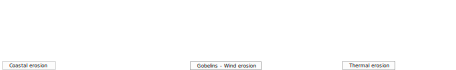
\includegraphics{figures/teaser.pdf}
	\centering
	\caption{Applying shading and textures on the generated geometry can produce a plausible aspect of a coast eroded by waves on a long timespan, or a desertic landscape eroded by wind, or a mountainous area flatten by thermal erosion.}
	\label{fig:erosion_closerImage}
	\label{fig:erosion_teaser}
\end{figure*}

\section{Introduction}
Automated terrain generation is a key component of natural scene digital modeling for animated movies and video games. A standard approach is to first generate a base terrain geometry using noise to define the height on the input domain \cite{Musgrave1989, Olsen2004, Roudier1993}, the result will most likely lack realism and feel synthetic. Erosion simulation algorithms are applied, to simulate thousands of years of ageing by reproducing physical phenomena - i.e. effects of the elements (rain, wind, running water...) - affecting the terrain making it more believable \cite{Stachniak2005, Smelik2009, Galin2019}.\\
The process of terrain alteration caused by the effect of water, air, or any other element - natural or not - over time is usually performed in three steps \cite{Neidhold2005}: \textbf{detachment} - pieces of the ground of variable dimensions, ranging from complete ledges to grains of sand, are removed from the terrain depending on the simulated meteorological phenomenon - \textbf{transport} - pieces of ground fallen from their initial position are moved to a different one (e.g. a cornice falls down a slope or a grain of sand is thrown into the air) - and \textbf{deposition} - transported pieces of land are accumulated at a new part of the landscape. Various phenomena can cause these alterations: \textbf{thermal erosion} (bursting of rocks caused by expansion of water under frost, then falling of debris to the bottom of a slope), \textbf{hydraulic erosion} (detachment caused by the impact of water particles on surfaces and the transport of sediments by the flow of runoff), \textbf{wind erosion} (fine particles carried away in the wind and hit surfaces on their way, creating new fine particles which then also fly away), \textbf{chemical erosion} (chemical decomposition of rocks caused by rainwater or other fluids), other exceptional phenomena such as avalanches, animals, lightning, etc... modify the terrain \cite{Cordonnier2017a, Argudo2020, Cordonnier2018, Cordonnier2017b,Cordonnier2023}. 

\begin{figure*}
\centering
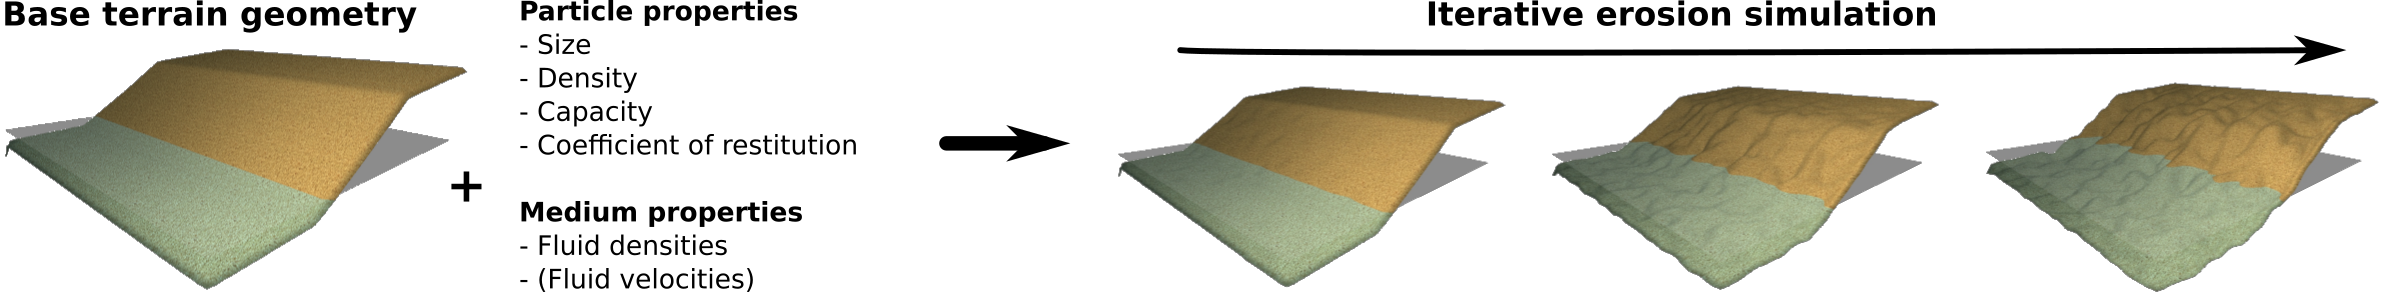
\includegraphics{figures/pipeline.png}
\caption{Our method require a base geometry, a small number of parameters for the particles and the medium used for the erosion simulation. It can be easily adapted to be compatible with different mediums and terrain representations.}
\label{fig:erosion_pipeline}
\end{figure*}

In practice, the core idea to simulate erosion is to add or remove material from the terrain at given positions on the interface between the terrain and fluid eroding it (e.g. air or water). Hence, the two major problems to tackle are: how to locally alter the terrain geometry for material detachment and deposition and where to perform these alteration given the properties of the environment (terrain slope, fluid density and velocity).
A terrain is more than often represented in 2.5D using a 2D image called a heightmap which grey scale values define terrain elevation. While being the major terrain representation, only a limited number of environments can be modeled. Indeed, natural landscapes are intrinsically 3D (overhangs, cavities or geological structures such as arches or gobelins), this is particularly true for underwater environments generation. Alternate representation such as voxel grids, material layers or implicit surfaces can be used. A wide variety of method have been proposed to simulate natural erosion phenomena on heightmaps as the partial differential equations to model erosion can be discretized and solved in 2D and the material detachment and deposition at a given point of the terrain surface can be easily performed by elevating or lowering the ground level i.e. changing locally pixel intensities. 
For volumetric representations, the alteration of the terrain is not as trivial.
To define where to perform the erosion process the local slope variations are more than often used combined with eroding medium information. This fluid can be simulated using particle systems, Smoothed Particle Hydrodynamics (SPH) \cite{Kristof2009} or approximated using a simple vector field. 
Proposed methods offer a specific erosion effect tailored to a single terrain representation and fluid simulation.

In this work we propose an approach to simulate a large part of the geomorphological and meteorological phenomena present in the literature of terrain generation (including 3D and volumetric effects). We introduce a generalized algorithm performing the three stages of erosion on surface and volume representations alike, and expose very few intuitive parameters to be adjusted by the user (Figure~\ref{fig:erosion_pipeline}).
We propose to tackle separately the material variation and the fluid simulation. Our method relies on a particle system to simulate eroding agents, each thrown particle will collide with the terrain, perform terrain alteration at the collision point and transport material along its path. 
Their motion is computed using simple particle physics accounting for the medium density and particle properties (buoyancy and gravity forces). We consider each particle as independent, hence, they do not interact with each other, no collision detection or response. This simplification allows for efficient parallel computation. 
When more accuracy or control is needed, we propose to provide a vector field used to modify the particle speed at each time step. The nature of this vector field is flexible, it can be computed using a more or less accurate fluid simulation (SPH, FLIP,...) or be manually defined by the user. We propose a particle-based strategy for material alteration that can be applied on surface and volumetric representation. \\
The main contributions of this paper are: 
\begin{itemize}
\item a generalized particle-based algorithm performing the three
stages of erosion on surface and volume representations,
\item decoupling the erosion system from the fluid simulation, making the process more flexible in its usage and implementation and opening the door for richer effects that can easily be produced.
\end{itemize}
% -----------------------------------------------------------------
\section{State of the art}
\label{sec:erosion_state_of_the_art}
In this section, we first present the major terrain representations (height fields, layered representations, voxel grids, and scalar functions) and a subset of the major simulated phenomena used to erode terrains. We highlight the fact that, in the literature, a specific erosion method tailored to a given terrain representation is proposed for given phenomena which might lead to limitation in term of terrain modeling. Indeed, changing representation costs information and precision loss.
\subsection{Terrain Representations}
A terrain can be represented in various ways, each of them suited for a given application of which we give an brief overview, more details can be found in \cite{Galin2019}.\\
\textbf{Height Fields} represents the surface of the terrain by defining the elevation at each point in a 2D grid. This representation is simple, regular, and fast to process allowing for easy manipulation, such as raising or lowering the terrain \cite{Gain2009, Emilien2015}.\\
\textbf{Layered Representations} are an extension of height fields using a 2D grid where each cell represents a stack of different materials instead of a simple height \cite{Peytavie2009, Benes2001} allowing for memory efficient representation of volumetric terrains. To create complex structures, arches or caves, solid materials can be transformed into more granular ones, that can be stabilized \cite{Peytavie2009}.\\
\textbf{Voxel Grids} are regular, uniform volumetric grids that encode information on the presence or absence of material for each 3D point in the domain. Voxel grids are advantageous due to their regularity \cite{Dey2018} and ability to represent volumetric models at the cost of high memory footprint, which has limited their use in terrain generation \cite{Ito2003, Kaufman1993, Lengyel2010a}. We consider two voxel grid representations : \textit{density-voxel} grids for which each voxel contains a scalar value, for instance the occupation percentage \cite{Eisemann2008}  and \textit{binary voxel} grids that can be seen as a mask containing the presence of material information.\\
\textbf{Implicit terrains} represent landscapes as an implicit surface defined by a scalar function. This allows for high definition large terrain modeling. The application of combinable scalar function overlays \cite{Guerin2016a} or the definition of user-defined gradients \cite{Guerin2022} can be used to create complex terrain features. Altering a implicitly defined surface is a challenging task hence limited option exist for erosion simulation \cite{Paris2019}.

\subsection{Erosion Processes}
Erosion processes play a crucial role in shaping landscapes over time. We present different kind of erosion and how they apply to given terrain representations. Note that using existing methods all erosion methods can not be used on all representation.\\
\textbf{Thermal Erosion} is driven by large temperature shifts, transferring material based on slope thresholds. The process is iterative, redistributing material until slopes stabilize. It can be computed efficiently on height fields and layered terrains due to their manipulable height nature \cite{Musgrave1989, Benes2001, Peytavie2009}. However, its application on voxel grids is challenging due to limited Z-axis resolution.\\
\textbf{Hydraulic Erosion} stems from water movement, eroding and depositing sediment based on water flow intensity. 2.5D terrains are widely studied for this simulation, using either water slope velocities \cite{Neidhold2005} or water simulations for erosion effects \cite{Mei2007}. For smaller scales, 3D fluid simulations on voxel grids have been proposed \cite{Benes2006}. Kristof et al \cite{Kristof2009} used SPH (Smoothed Particle Hydrodynamics) for meshless erosion simulations on various terrains. Their method involves numerous particle interactions, demanding significant computational power. Our approach draws inspiration from this but enhances efficiency by removing certain particle interactions.\\
\textbf{Wind Erosion} shifts material through wind force, notably impacting areas with fine surface particles like deserts. It has been modeled on discrete height fields \cite{Roa2004, Paris2020} by mimicking sand's wind-driven trajectory and using thermal erosion for corrections. This process is simulated by iteratively displacing small amounts of matter, which make it less suitable for representations with discrete height resolution.\\
\textbf{Erosion by Other Forces} includes influences like glaciers, snow, tectonic movements, and fauna, each introducing distinctive terrain patterns, enriching its intricacy \cite{Cordonnier2016,Cordonnier2017a,Cordonnier2018,Cordonnier2017b,Argudo2020}. However, most methods are tailored by a given terrain representation, often the height fields, and might not be applicable to other representations due to their intrinsic properties.
%--------------------------------------------------------------------------
% \section{Technical background}
\section{Particle erosion}% [instead of "Technical background"]}
\label{sec:erosion_method}
Erosion occurs in three stages: material detachment, transport and deposition (respectively in red, black and green in Figure~\ref{fig:erosion_ablation_erosion}). In our approach, particles move through the medium following its flow (i.e. wind in air or currents in water) and then absorb or deposit a small amount of material upon contact with the land surface, effectively fulfilling the three stages of erosion.
\begin{figure}[ht]
\centering
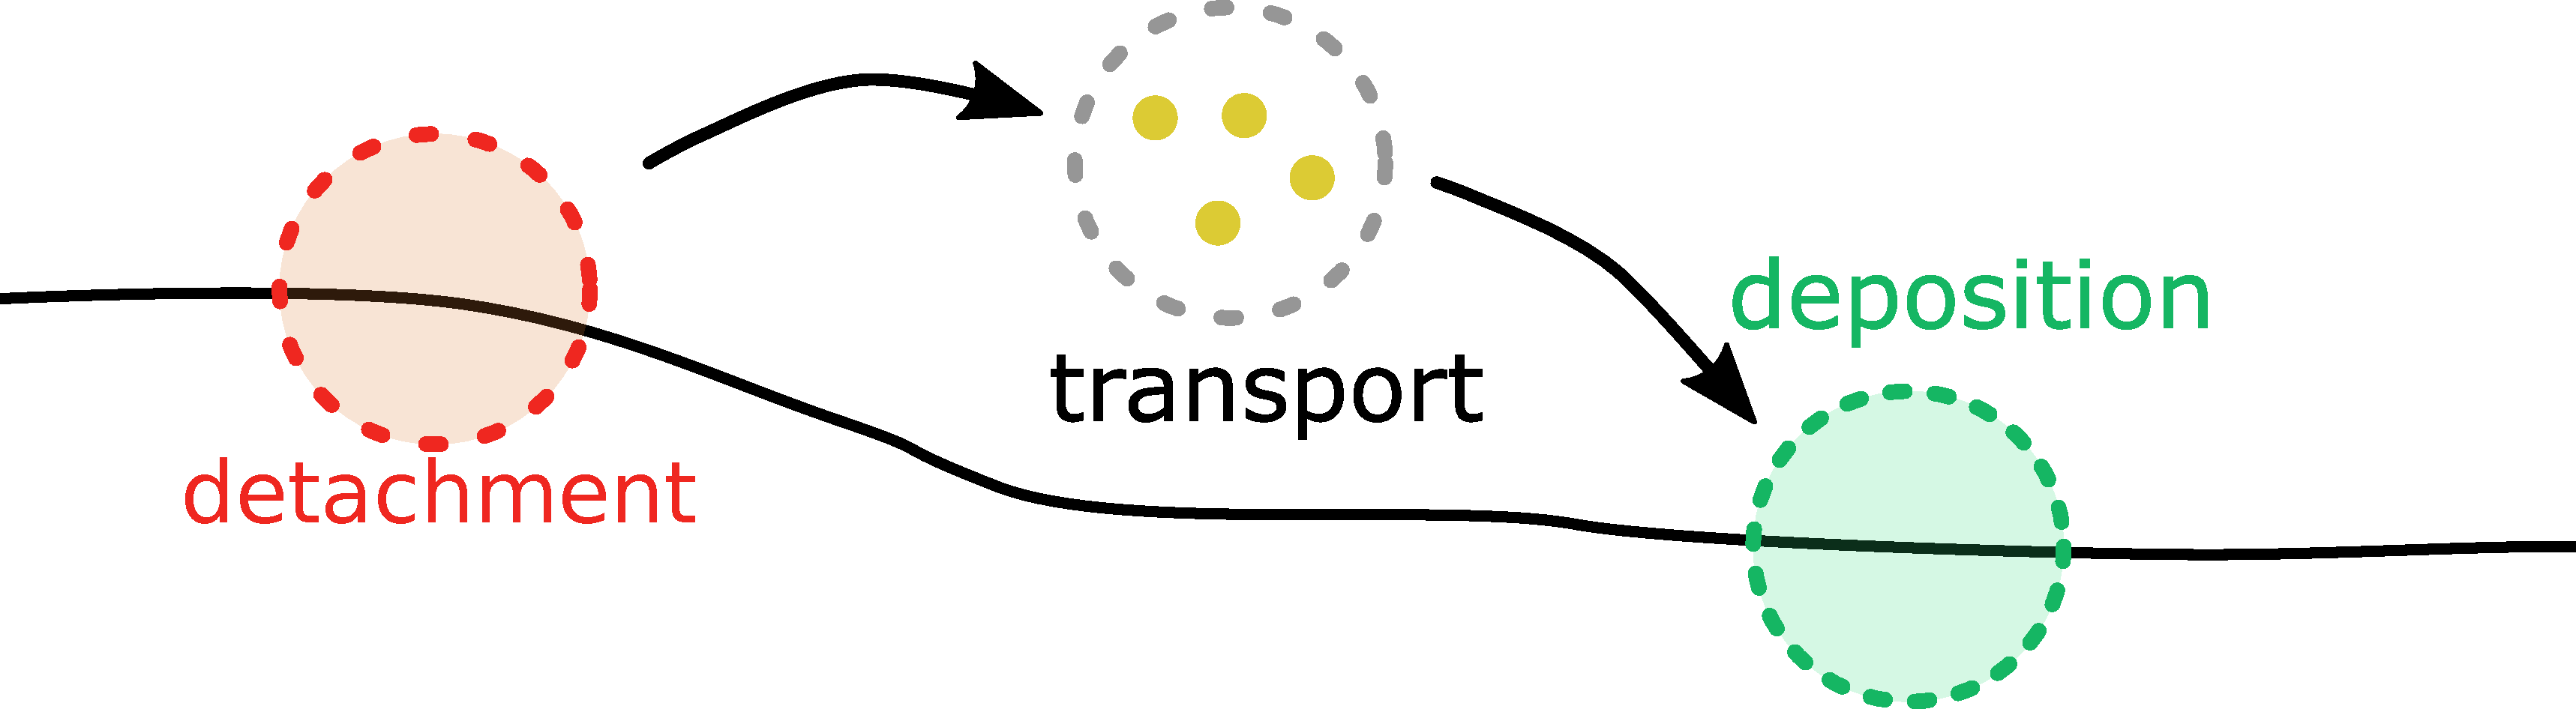
\includegraphics[width=0.95\linewidth]{figures/ablation_erosion.pdf}
\caption{Three steps of the erosion process from the sediment point of view: detachment from its original location - dotted red circle -, transport in a fluid - dotted black circle -, deposition at a new location - dotted green circle.}
\label{fig:erosion_ablation_erosion}

\end{figure}
\subsection{Overview}
Particles are transported through the medium and can pass through several different media. Each medium is defined by a density and a flow. Consider, for example, water density to be \SI{1000}{\kilogram \per \cubic \meter} and that of air to be \SI{1}{\kilogram \per \cubic \meter}. The gravity applied to the particles is then very different between open and submerged environments due to the difference in buoyancy, while the process remains similar.
Using a pre-calculated flow field to guide particle movement simplifies the simulation by treating particles as independent entities, eliminating the need for inter-particle calculations. This not only reduces significantly the overall execution time but also offers users high flexibility over the quality of the simulation and simplify the implementation. 
\subsection{Erosion process}
\begin{wrapfigure}{r}{2,4cm}
\centering
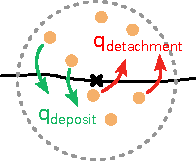
\includegraphics{figures/erosion_deposition.pdf}

\end{wrapfigure}
Every time the particle hits the ground, a given amount $\erosionAmount$ of sediment is detached from the ground (red arrows) while another amount $\depositAmount$ of sediments is deposed at this location (green arrows). Our erosion model is based on the work of Wojtan et al where regular 3D grids are used to estimate the fluid velocity and sediment transport \cite{Wojtan2007}. In the spirit of \cite{Kristof2009}, we transposed their method into a particle-based erosion simulation, but, in our proposition, we decouple the particle system from the fluid simulation, making the process more flexible and opening the door for richer effects that can easily be produced. 

\textbf{Detachment.}
As a particle approaches the surface of the terrain, its motion applies friction at the interface between fluid and ground, causing bedrock to dislocate microscopic parts, that we call abrasion. We use pseudoplastics model to approximate the amount of matter removed due to the shear forces while considering the physical properties of the fluid and the ground \cite{Wojtan2007}. 

The shear rate $\shearRate$ is approximated by the relative velocity of the fluid to the solid boundary $\velocity_{rel}$ over a short distance $l$.
We approximate the shear stress $\shearStress$ at the solid boundary by a power-law:
\begin{align}\label{eq:shearStress}
\shearStress = \shearStressConstant \shearRate^n
\end{align}
where $\shearRate = \velocity_{rel}/l$, $\shearStressConstant$ is the shear stress constant (often set to $1$) and $n \in [0,1]$ is the flow behaviour index. Shear-thinning models typically assume $n$ close to $\frac{1}{2}$, which is why we used this value as a constant.  

We can then compute the erosion rate $\erosionRate$ at any contact point between a fluid and a solid boundary using \eqref{eq:shearStress} by 
\begin{align}\label{eq:erosionRate}
\erosionRate = \erosionStrength (\shearStress - \criticalShearStress)^a
\end{align}
with $\erosionStrength \in [0,1]$ a user-defined erosion constant, $\criticalShearStress$ the critical shear stress value for which the matter starts to behave like a fluid and $a$ a power-law constant, typically considered as $a = 1$. 

In our method, the eroded quantity is approximated as the material contained in the half sphere, of radius $\particleSize$, in the normal opposite direction at the particle impact point (Figure~\ref{fig:erosion_erosion_heightfield}). We then use \eqref{eq:erosionRate}: 
\begin{align}\label{eq:erosionAmount} 
\erosionAmount = \erosionRate \frac{ 2 \pi \particleSize^3 }{ 3 }
\end{align}
to get the final eroded amount $\erosionAmount$. The particle is also defined by a maximal amount of sediments that can be contained in its volume before being saturated noted $\maxCapacity$. Note that this constant will be used for the settling velocity computation \eqref{eq:initialSettlingVelocity}.

\textbf{Deposition.}
The eroded sediments are considered in suspension in a fluid and are affected by its velocity. A fluid particle then transports the sediments in its flow until gravity settles it onto the ground again. The effect of gravity is modeled by a settling velocity $\settlingVelocity$ defined in Eq~\eqref{eq:initialSettlingVelocity}. We consider that the amount of sediment settled is proportional to the norm of the settling velocity as proposed in \cite{Wojtan2007} with $\depositionRate \in [0,1]$: 
\begin{align}\label{eq:deltaDepositon}
\depositAmount = \depositionRate ||\settlingVelocity||.
\end{align}
% The corrosion simulation can be performed by setting $\lambda_{deposit} = 0$.


\subsection{Transport}
Our simulation is computed by integrating the full trajectory of multiple particles at each iteration unlike most other erosion methods. This allows to constantly have a terrain in a plausible state, while giving the possibility to increase the aging effect by running more iterations. 
Note that, reducing progressively the overall erosion strength can be used as a strategy to adapt the computation time to a chosen level-of-details.

We first present how to compute the particle speed using particle's physics then how to add optional medium velocity field to add a fluid simulation or user control.

\textbf{Particle's physics.}
From its independence with other particles: we consider each particle following Newton's laws of motion.\\
First, we define the external forces $\extForce$ applied on each particle, we consider gravity and buoyancy.
We calculate the buoyancy force $\buoyancyForce = -\fluidDensity \volume \gravity$ with $\fluidDensity$ the density of the fluid, $\volume$ the volume of the particle and $\gravity$ the gravitational acceleration, but we can also calculate the force of gravity $\gravityForce = \particleMass \gravity$ with $\particleMass$ the mass of the particle. We then have the final external force $\extForce = \gravityForce + \buoyancyForce = \particleMass \gravity - \fluidVelocity \volume \gravity$ knowing the density of an object $\particleDensity = \frac{\particleMass}{\volume}$, we have:
\begin{align} \label{eq:gravity}
\extForce = \volume \gravity (\particleDensity - \fluidDensity ).
\end{align}
The particle velocity $\velocity$ can be integrated from \eqref{eq:gravity} by: 
\begin{align} \label{eq:velocity-computation}
\velocity = \int{ \extForce \, dt} + \settlingVelocity + \velocity_0,
\end{align}
with $\settlingVelocity$ the settling speed of sediments in a fluid with a viscosity $\viscosity$ given by Stoke's Law \cite{Stokes1850}: 
\begin{align} \label{eq:initialSettlingVelocity}
\settlingVelocity = \frac{ 2 }{ 9 }  \gravity \particleSize^2 \frac{(\particleDensity - \fluidDensity)}{\viscosity } f(\capacity).
\end{align} 
We use the Richardson-Zaki relation as the hindered settling coefficient: \\
$f(\capacity) = 1 - \left( \frac{\capacity}{ \maxCapacity } \right)^{n}$ \\
with $\capacity$ and $\maxCapacity$ respectively the fraction of volume of sediments contained and the maximal fraction of sediments the particle can contain, and $n$ an exponent typically 4–5.5, which we set to 5 \cite{Richardson1954, Wojtan2007}.

Finally, the particle position can be integrated as: 
\begin{align} \nonumber
\p = \int{ \velocity \, dt} + \p_0.
\end{align}
When the particle hits the ground, a coefficient of restitution affects its behaviour by reducing its velocity post-collision. This value depends on ground material as it is influenced mainly by the material's particle shape, coefficient of friction and density \cite{Yan2020}. Less bouncy particles lose speed quickly and settle down sooner, forming a steeper pile (Figure~\ref{fig:erosion_coefficient of restitution-diagram} blue), or a higher talus angle like chalk. On the other hand, more bouncy particles disperse more widely upon hitting a surface, resulting in a gentler accumulation like clay (Figure~\ref{fig:erosion_coefficient of restitution-diagram} red).
\begin{figure}
\centering
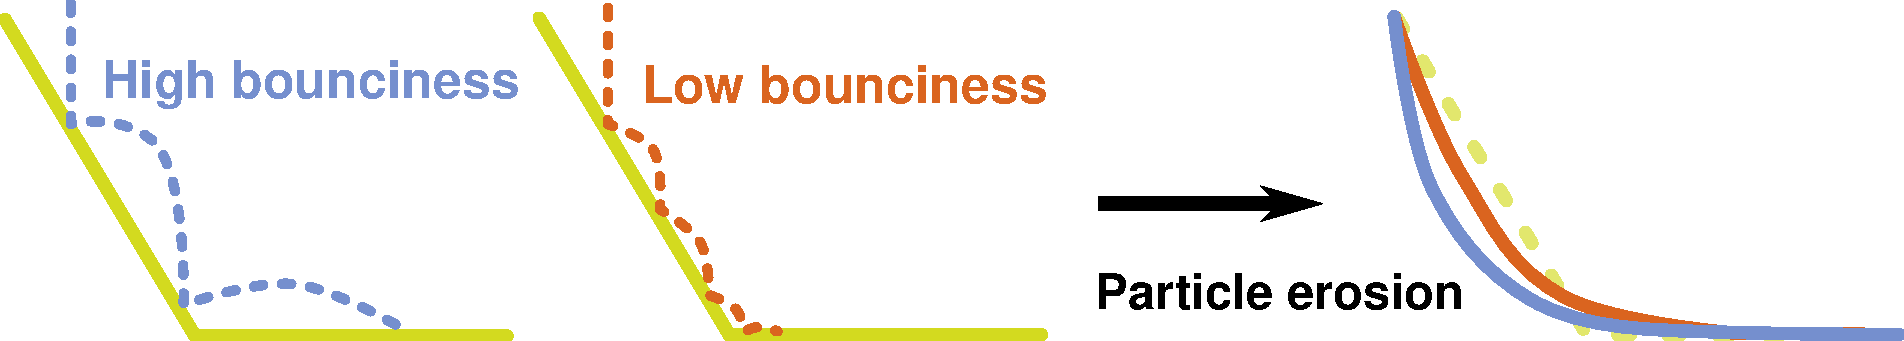
\includegraphics{figures/bounciness.pdf}
\caption{The coefficient of restitution affects the amount of energy absorbed from the particle when hitting the ground. Here, rain is applied on an initial slope (yellow). Only two particles are displayed, with a high (blue) and low (red) coefficient of restitution. The resulting slope after erosion is displayed in blue and red (right). }
\label{fig:erosion_coefficient of restitution-diagram}

\end{figure}

\textbf{Velocity field.}
\label{sec:erosion_velocity_field_refinement}
In our model, we allow the user to add a velocity field to the environment that influences particles motion. This velocity field can be the result of a complex fluid simulation, a uniform vector field, or an artistic motion field.
We modify Equation \eqref{eq:velocity-computation} such that the particle's speed will be influenced by the velocity field as follows:
\begin{align} \label{eq:velocity-computation-final}
\velocity = \int{ \extForce \, dt} + \settlingVelocity + \alpha \fluidVelocity + \velocity_0,
\end{align}
with $\fluidVelocity$ medium velocity field modulated by $\alpha \in [0,1]$. 

Our particle system can model intricate scenarios, like the erosion caused by water currents on the seabed or aeolian erosion. The velocity field remains static during the erosion, which may cause inconsistencies in the fluid velocity field. However, minor changes can be overlooked to maintain a balance between realism and computational efficiency \cite{Tychonievich2010}. We offer several velocity improvement methods: \\
\textbf{-Fluid simulation refinement:} Many erosion systems incorporate fluid simulation, requiring regular updates for erosion and velocity \cite{Kristof2009, Wojtan2007}. Our method can use fluid simulations with multi-resolution refinement, with the possibility to focus the velocity field adjustments near the updated boundaries of the surface \cite{Roose2011}. \\
\textbf{-Particle velocities in fluid simulation:} With a Lagrangian fluid simulation relying on particle systems \cite{Koschier2022}, our particle velocities can be incorporated in its computation. This approach is only a provisional solution due to potential parameter mismatches with main fluid simulation. \\
\textbf{-Velocity field diffusion:} Given the minor changes to the surface level at each erosion iteration, which reflect the gradual alterations in terrain surface, we can estimate that the velocity at a fixed point transitioning between the inside and outside of the terrain closely mirrors the velocities observed in its surrounding area. In this context, we can simply interpolate the velocity field at any transitioning point. This simple method, as used in Figure~\ref{fig:erosion_underwater_result}, allows us to find a balance between achieving realistic flow simulations and maintaining computational efficiency.
% Our contribution part
% ------------------------------------------------------------
\section{Our erosion method}
\label{sec:erosion_application_on_representations}
\begin{figure}[t]
    \centering
    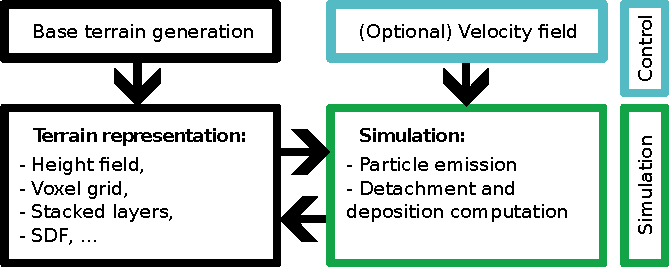
\includegraphics{figures/figure_pipeline.pdf}
    \caption{Our overall pipeline: our erosion process compute matter displacement of a terrain using an arbitrary representation as long as intersections between particles and the ground can be detected. An optional velocity field, provided by the user, guides the particles trajectories. We propose surface alteration methods to apply the erosion to the terrain in a coherent way between possible representations. }
    \label{fig:erosion_figure_pipeline}
\end{figure}
In this section, we describe how to apply detachment and deposition to different terrain representations with our method (Figure~\ref{fig:erosion_figure_pipeline}). We cover the most commonly used representations namely height fields, layered terrains, voxel grid and implicit surfaces, note that our work could be extended to additional representations. Two conditions need to be satisfied for a representation to be eligible for our erosion method: being able to evaluate the intersection of a particle with the ground and compute the normal of the terrain at this point. To the best of our knowledge, all representation do. \\
We use Verlet integration for the particle's physics  \cite{Verlet1967}, with low error rate and stability even for high $dt$, reducing computation time for negligible imprecision \cite{Baraff1998, Swope1982}.

For all the representations, the amount of material absorbed by the particle, i.e. the erosion value $\erosionAmount$ from \eqref{eq:erosionAmount}, is taken around the particle at a radius $\particleSize$, meaning that the modification of the terrain by a particle at position $c$ will only occur for the positions $\p$ satisfying $||\p - c|| < \particleSize$. At the same time, the amount $\depositAmount$ from \eqref{eq:deltaDepositon} is deposited, resulting in a change $\totalErosion = \depositAmount - \erosionAmount$\\ 
In our simulation, while the dynamics are informed by physical principles, the particle size is conceptualized within a dimensionless framework. This provides the flexibility to adapt our results to various real-world scales, ensuring the applicability of our model across diverse scenarios.
Note that, for a 2.5D terrain, we can consider that half of the sphere surrounding the particle is affected which has a volume of $V_{2.5D} = \frac{2 \pi \particleSize^3}{3}$ while a 3D terrain is affected by the full sphere $V_{3D} = \frac{4 \pi \particleSize^3}{3}$ (as illustrated  Figure~\ref{fig:erosion_erosion_heightfield}). In the following sections, we will describe the strategies used to modify the amount of matter for different representations. 
\begin{figure}
\centering
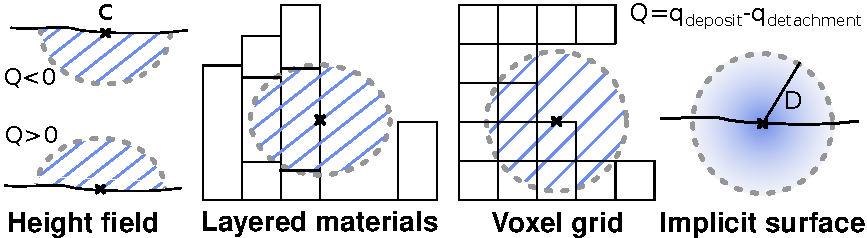
\includegraphics{a_erosion_deposition.pdf}
\caption{Illustration of the material detachment in the (half-)sphere at contact point $C$ (cross) on different representations. (height field) When $\totalErosion < 0$ material detachment happen in the bottom scaled half sphere of the particle's contact with the ground, while the deposition is applied on the upper half sphere of volume when $\totalErosion > 0$. Unlike the height field, for 3D terrains detachment and deposit are applied in the full sphere around the contact point.}
\label{fig:erosion_erosion_heightfield}

\end{figure}
\subsection{Application on height fields}
\label{sec:erosion_application_on_heightmaps}
On a height field defined by $h(\p) = z$, the intersection point with the surface is verified at $\p_z = h(\p)$, and the normal can be computed at the intersection point. 

For this representation, the half sphere is scaled in the $z$ direction to fit $\alpha \volume = \totalErosion$ using $\alpha = \frac{\totalErosion}{\volume}$. We then can decrease the height $h'(\p)$ at all points $\p$ by the height of the scaled half sphere at position $\p$. Given the height of the scaled half sphere of center $c$ and the distance of the particle to the center $d = ||\p - c||$ by $h_\text{half sphere}(\p) = \alpha \sqrt{\particleSize^2 - d^2}$ for all $\p$ such that $d \leq \particleSize$ the radius around a particle.

This change of height can be sampled at all points of the 2D grid by reducing the height by 
\begin{align} 
\label{eq:erosionHeightfield}
\Delta h(\p) &= \frac{\sqrt{\particleSize^2 - d^2}}{\alpha} = \frac{\totalErosion}{\frac{2}{3} \pi \particleSize^3} \sqrt{\particleSize^2 - d^2}
\end{align}
The height at each point after an erosion is then computed as $\Tilde{h}(\p) = h(\p) + \Delta h(\p)$.

\subsection{Application on layered terrains}
\label{sec:erosion_application_on_layers}
Layered terrains are defined as $\mu: \R^3 \to \N$ assigning a discrete material index $\mu$ for any point in space \cite{Benes2001, Peytavie2009}. In the original work, outer borders stack elements of the terrain are transformed into density-voxels to enable global erosion through height changes. We enable the erosion/deposition process directly on the layers hence removing the need for representation changes. \\ 
When intersecting the terrain, the amount eroded for each material stack should be the integration of the volume of the intersection between the sphere surrounding the particle and the cubicle represented by the stack. Since there is no easy solution \cite{Jones2017}, we approximate the volume of the stack we need to alter using the previously defined height field equation \eqref{eq:erosionHeightfield}. 
At a distance $d$ from the particle, the height is defined as:
\begin{align} \label{eq:erosionLayers}
H(d) = \frac{|\totalErosion|}{\frac{2}{3} \pi \particleSize^3} \sqrt{\particleSize^2 - d^2}.
\end{align}
If $\totalErosion > 0$ (more deposition is applied that detachment) then we transform the materials in the stack contained in the sphere to become ground material. For $\totalErosion < 0$ the materials are transformed in background material.

\subsection{Application on implicit terrains}
\label{sec:erosion_application_on_implicit}
Implicit terrain are defined using a function $f(\p)$ and its variation resulting from the erosion process using $\Delta f(\p)$.
We propose a strategy to compute $\Delta f(\p)$ at any point of the sphere surrounding the erosion point based on metaball primitives. At each contact point a metaball is added to create a hole or a bump in the terrain. A metaball is defined as: 
\begin{align}\label{eq:erosionMetaball}
\Delta f(\p) = \frac{3 \totalErosion}{\pi} \frac{(1 - d)}{\particleSize}
\end{align}
with $d$ the distance of the point $\p$ to the sphere center. For all point $\p$ for which $d \geq \particleSize$, $\Delta f(\p) = 0$ (see \ref{sec:erosion_appendix_metaball}).

As they are the most commonly used representations, we propose a formulation to erode implicit terrains defined by Signed Distance Functions (SDF) and by gradient or vector fields.

\textbf{Signed Distance Functions}
\label{sec:erosion_application_on_sdf}
Considering SDF, the terrain is defined as the 0-set of the signed distance function $f: \R^3 \to \R$, hence, for $f(\p) = 0$, the inside as $f(\p) < 0$ and outer-part (i.e. air or water) as $f(\p) > 0$. \\ 
The particle erosion applies at impact points at discrete positions, so we propose to add or subtract metaballs defined using equation~\eqref{eq:erosionMetaball} to respectively deposit or erode material using a composition tree:\\ $metaball(\p) = -\Delta f(\p)$.\\
Now the eroded terrain function $\Tilde{f}(\p)$ will be evaluated at each point $\p$ from the initial terrain value $f(\p)$, the erosion function $metaball(\p)$ and the composition function $g(f_1, f_2)$:
\begin{align} \label{eq:finalMetaball}
\Tilde{f}(\p) = g(f(\p), metaball(\p)).  \nonumber
\end{align}
As a metaball is added for each particle bounce on the terrain space partitioning optimization algorithms such as k-d trees, BSP trees or BVH can easily be used to improve performances.

\textbf{Other implicit terrains}
\label{sec:erosion_application_on_other_implicit}
are present in the literature, notably a 2.5D representation based on the surface gradient \cite{Guerin2022} and a 3D representation based on curves \cite{Becher2017} for which the trajectory of each particle projected to the closest surface could be used to define the alteration of the terrain.\\
In the case of gradient-based representation, we propose to use the partial derivative from the equation of the 2D scalar fields \eqref{eq:erosionHeightfield} that gives:
\begin{align} %\label{eq:erosion_gradients}
\nabla h' = - \frac{\totalErosion}{\frac{2}{3}\particleSize^3} \frac{1}{\sqrt{\particleSize^2 - d^2} } \vec{CP}
\end{align}
with $\vec{CP}$ the vector from the position $\p$ to evaluate to the center of the erosion point $c$.
Now the new gradient field can be computed as: 
$$
\nabla \Tilde{h}(\p) = \nabla h(\p) + \nabla h'(\p).
$$
\begin{figure*}
\centering
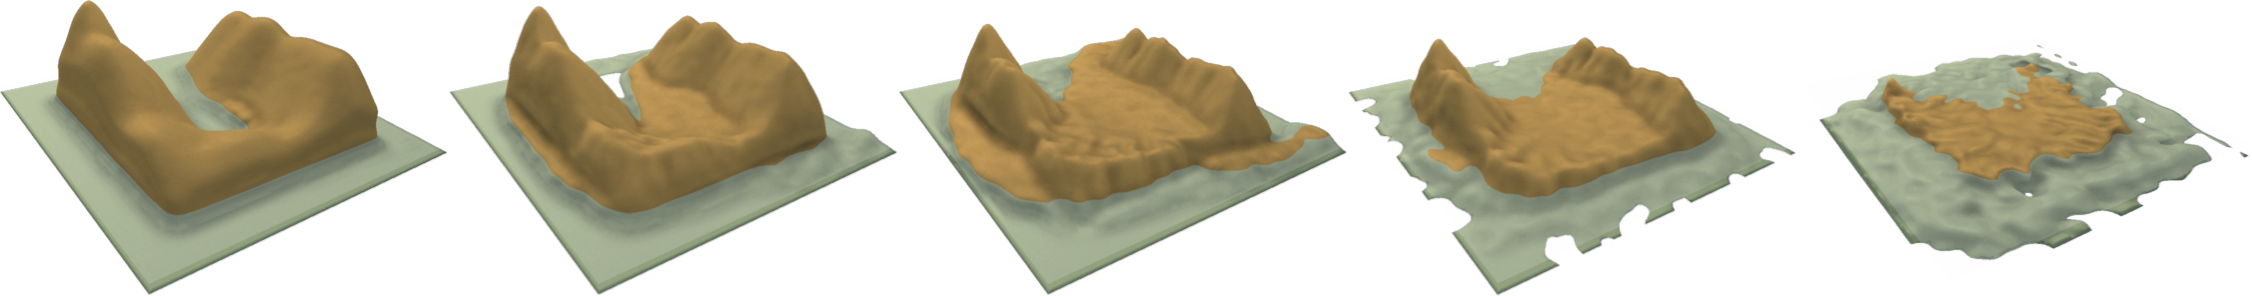
\includegraphics{figures/new_continuous_erosion2.png}
\caption{Our erosion method is applied iteratively on a completely synthetic island, the terrain is altered to obtain a plausible shape by forming rills. The use of particles with hydraulic densities dropped from the sky results in a strong erosion on the sides of the mountains, and the particles that slide to the sea are mainly drifting offshore resulting in the formation of small beaches and a weaker erosion on the bottom of the water body. Repeating the process causes the island height to decrease progressively up to the point where only the submerged part of the terrain is sheltered from erosion.}
\label{fig:erosion_continuous-erosion}

\end{figure*}

\subsection{Application on voxel grids}
\label{sec:erosion_application_on_voxels}
% \subsubsection{Density-voxels}
We consider two of the voxel grids representations: density-voxel grids and binary voxel grids for which we present our material alternation strategy.

\textbf{Density voxels.}
\label{sec:erosion_application_on_density_voxels}
We consider "density-voxel" grids defined on $f: \Z^3 \to [-1, 1]$ for which a voxel is be full for $f(\p) = 1$, partially full for $-1 < f(\p) < 1$ or empty for $f(\p) \leq -1$. 
This definition allows us to erode them smoothly. 
Since this kind of grid is a discretizaion of a scalar function, We could directly use \eqref{eq:erosionMetaball}, as described previously, but we take advantage of the discrete nature of the representation to avoid expensive computation. \\
We apply the erosion from a particle at position $c$ on all points $\p$ in the volume proportionally to the distance from the center of the sphere $d = ||\p - c||$ to find an approximation to the real erosion value per voxel $\totalErosion_{approx} = \totalErosion \frac{1 - d}{\particleSize}$.
Using their discrete nature, we rectify this value to sum up the total erosion value to $\totalErosion$ by dividing each value by the sum of the distances. We now consider eroding the "empty" voxels since their density can drop until $-1$. We then have for all surrounding voxels: 
\begin{align} \label{eq:erosionVoxels}
\Delta f(\p) = \totalErosion \frac{ (1 - \frac{d}{\particleSize} )}{ \sum {(1 - \frac{d}{\particleSize})}}.
\end{align}
Resulting voxel value is computed as $\Tilde{f}(\p) = f(\p) + \Delta f(\p)$.
In our implementation, when $f(\p) > 1$, we simply transport the density excess to the above voxel, giving it a very close analogy to height fields as long as $|\Delta f| < 1$. 

\textbf{Binary voxels}
\label{sec:erosion_application_on_binary_voxels}
The terrain can be represented using an occupancy function as $f: \Z^3 \to \{0, 1\}$ where a voxel $f = 1$ defines the ground and $f = 0$ the background. \\ 
We propose to apply particle erosion by assigning voxels a number of hits, and transform them as air or as ground when this number reaches a critical value $C$ that is proportional to the particle's strength parameter $\erosionStrength$ \cite{Jones2010}. \\ 
On a hit, all voxels in a radius $\particleSize$ receive a hit number: 
\begin{align} \label{eq:erosionDiscreteVoxels}
\Delta hits = \lfloor \alpha \Delta f \rfloor
\end{align}
with $\Delta f$ the erosion per voxel computed using \eqref{eq:erosionVoxels} and $\alpha$ a coefficient high enough to obtain values above 1. \\ 
All voxels with $\# hits > C$ are transformed to background and voxels with $\# hits < -C$ are transformed to ground.\\
Note that, a binary voxel grid can also be transformed into a density-voxel grid to be eroded smoothly.

Our formulation for height fields \eqref{eq:erosionHeightfield}, can be used to erode 2D scalar field-based representations. Similarly, 
our proposition for SDF \eqref{eq:erosionMetaball} enables erosion for continuous 3D scalar fields and voxels \eqref{eq:erosionVoxels} for discrete 3D scalar fields respectively.
% -----------------------------------------------------------
\section{Results}
\label{sec:erosion_erosion_examples}
% \begin{wrapfigure}{r}{3,5cm}
% \centering
% 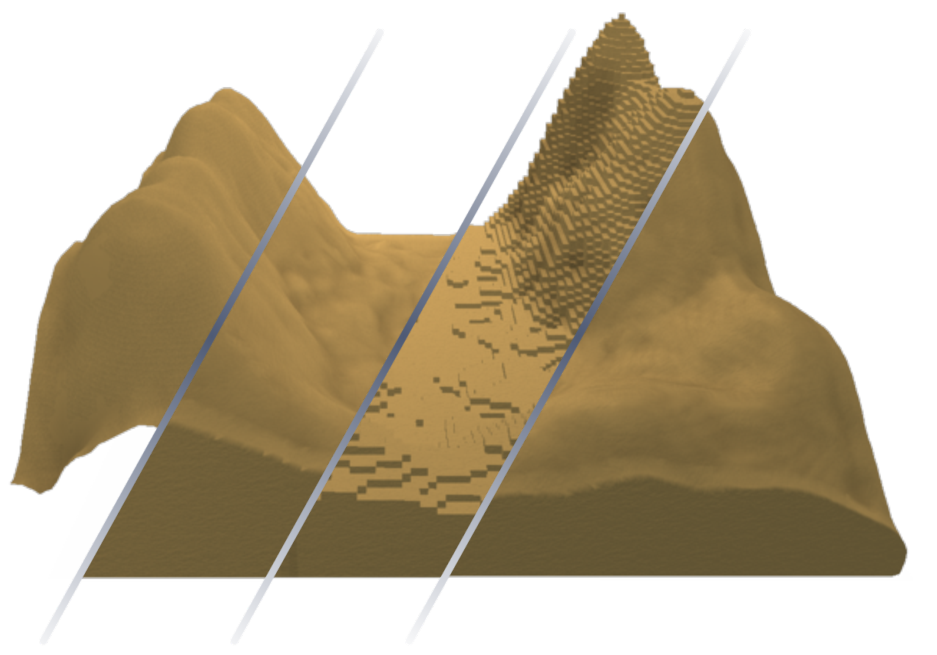
\includegraphics{figures/multi_representations.pdf}
% \label{fig:erosion_comparison-representations}
% \end{wrapfigure}
Our erosion process enables the simulation of a wide range of erosion effects on the major terrain representations alike. In this section, we present applications that demonstrate the versatility of our method by changing the particle's effect size, quantity, density, maximum capacity, deposition factor and the velocity fields. The results of each process are presented in Figure~\ref{tab:result_figures}, parameters used are available at Table~\ref{tab:result_parameters}. 
It is important to note that all erosion examples presented in this section are available for any 3D terrain representation. However, we cannot create volumetric structure, such as overhangs, using 2.5D representations (height fields).

Environment density $\fluidDensity$ is set to \SI{1}{\kilogram\per\cubic\meter} above water level (terrain blue part) and to \SI{1000}{\kilogram\per\cubic\meter} below it.
Velocity field's refinement is done by using the presented diffusion strategy.

\begin{table*}
    \centering
        \begin{tabular}{|lHlllllllllllll|}
            \hline
            \thead{Name} & \thead{Results} & \thead{Rep.} & \thead{Dimensions} & \thead{Res} & \thead{$\#P$} & \thead{$\#N$} & \thead{$\particleSize$} & \thead{$COR$} & \thead{$\particleDensity$} & \thead{$\capacityFactor$} & \thead{$\erosionRate$} & \thead{$\depositionRate$} & \thead{Vel field} & \thead{$t$} \\
            \hline
            \exampleHydraulic \\
            \exampleCoastal \\
            \exampleMeanders \\
            \exampleRiverTwo \\
            \exampleLandslide \\
            \exampleVolcano \\
            \exampleKarstBinary \\
            \examplePipes \\
            \exampleWindErosion \\
            \exampleWaterCurrents \\
            \hline
        \end{tabular}
        \caption{Parameters used for the generation of the terrains presented in Figure~\ref{tab:result_figures}, with "Rep" the representation  (\heightmap: Heightmap, \densityVox: Density-voxels, \binaryVox: Binary voxels, \implicit: Implicit) "Res" the resolution in meter per voxel or cell, $\#P$ the number of particles per iteration, $\#N$ the number of iterations, $\particleSize$ the particles radius (in voxel or cell unit), $COR$ the coefficient of restitution, $\particleDensity$ the particle density in \SI{}{\kilogram\per\cubic\meter}, $\capacityFactor$, $\erosionRate$ and $\depositionRate$ respectively the capacity, erosion and deposition factors, "Vel field" the type of velocity field used and $t$ the computation time of the simulation in seconds on CPU. \\ $^{(1)}$ The velocity field is a vector field defined as $\fluidVelocity(\p) = [0 ~ sin(\p_x) ~ 0]^T$.}
        \label{tab:result_parameters}
        
\end{table*}

\textbf{Rain.}
Hydraulic erosion from rain is the most common process used in terrain generation. In this case, particles are seen as water droplets falling from the sky and rolling downhill due to the gravitational force of Earth. No velocity field is required from fluid simulation. These parameters result in a detailed geometry of the rills on the side of mountains that quickly emerge and deposit many sediments in the valley.  
We demonstrate the result of rain erosion in \referenceExemple{Rain} with a computation time of 4 seconds.  \\
Using this erosion parameters in combination with water bodies results in different outcomes (Figure \ref{fig:erosion_continuous-erosion}). The terrain above water is directly affected by the erosion process while particles colliding with the underwater part of the terrain are slowed down and filled with sediments, leading to mainly apply deposition. The result is a typical hydraulic erosion on mountains and the formation of slopes and beaches near water level.

\textbf{Coastal erosion.}
Waves repeated motion  creates coastal erosion, that can be seen as cliffs with holes at the water level. \\
We apply a uniform velocity field in the water pointing towards the coast to simulate waves and emit particles from the water area with a large size, a density between air and water densities, a high capacity factor and a low deposition factor $\depositionRate$. Using these parameters, the erosion process is focused at the interface of air and water, and apply a coarse detachment while depositing a very small quantity of sediments, simulating the corrosive effect of water on limestone. \\ 
This effect can only be simulated on 3D terrain representations, but will create cliffs on a 2D representation. 
\referenceExemple{Coastal} presents the result of coastal erosion on a density-voxel grid that creates overhangs around sea level using a small amount of particles. Note that, the same effect using an alternate implicit representation based on SDF is displayed in Figure \ref{fig:erosion_screen-paris2019-1}.
A shaded version of this effect is presented in Figure \ref{fig:erosion_closerImage}.

\textbf{Rivers.}
Given a source point, we generate particles that run downhill, simulating the formation of a river. More complex erosion simulation using fluid simulations like SPH \cite{Kristof2009} would create realistic results at the cost of high processing time. Our method offers the flexibility to be applied either with a velocity field (simple, used given or resulting from a fluid simulation) or without allowing for simplicity and efficiency.\\
When provided with a hand-made or procedural velocity field, our particle system can reproduce simple river meanders (\referenceExemple{Meanders}). \\ 
\referenceExemple{River} presents a river that has been modeled by emitting water particles with different sizes that ranges from \SI{1.5}{\meter} to \SI{5}{\meter}, a high coefficient of restitution and a low capacity factor. Random sizes are used to simulate a river for which the flow rate had fluctuated over formation time, while the low capacity ensure that the banks of the river stays smooth. A high coefficient of restitution is a strategy that let the particles flow with low friction, approaching a water behaviour. Our particles are affected only by gravity, without fluid simulation.

\textbf{Landslide}
are mainly caused by large amount of water saturating the ground and flowing downhill, transporting matter in its path. \\
By using water particles with a medium size, a low coefficient of restitution and a low capacity factor but a high deposition factor $\depositionRate$, they transport sediments on short distances as the velocity quickly drops to 0, and ground material is completely spread along its path since it is easier to deposit the same amount of sediment than the eroded amount at each collision point. Reducing the density of the particle simulates a rise of viscosity in the settling velocity formula, increasing again the quantity of matter to deposit at contact with the ground. By this means, we can simulate landslides as illustrated on \referenceExemple{Landslide}. A smoother surface is resulting, compared to the rain erosion as the rills are filled with sediments as soon as they begin to form.
%
By setting the initial capacity of the particle equal to 10\% of its max capacity, the mass of the terrain increases, simulating a volcano eruption as illustrated on \referenceExemple{Volcano}.

\textbf{Karsts} networks are created over hundreds of years from the corrosion of water on the limestone in the ground. A limited number of methods have been proposed for the procedural generation of karsts \cite{Paris2021}.\\ 
By reducing the deposition factor $\depositionRate$, the particles simulate corrosion (without mass conservation). We can use the same particle parameters than the coastal erosion (big size, a density between air and water densities, a high capacity factor and a low $\depositionRate$) and optionally provide a 3D shear stress map. The karst will automatically follow the softest materials, which is geologically coherent as given in example in \referenceExemple{Karst}, where we can observe a "pillar" that is formed in the center, and thus the karst forms two corridors that finally merge partially. 
%
Underground results are only available for representations allowing 3D structures. Another underground terrain simulation is shown in \referenceExemple{Tunnel} in which a water runoff is eroding a tunnel without the use of a fluid simulation. Here, when particles bounce often on the terrain surface, the coefficient of restitution may be seen as a viscosity parameter.

\textbf{Wind}
erosion is a significant process in desertscapes shaping since there are no obstacles on the airflow path. Air particles can reach high velocities, transporting sand over long distances forming either dunes or are blasted into rocks, eroding into goblins. \\ 
By setting the density of our particles close to \SI{1}{\kilogram\per\cubic\meter}, two erosion simulations can be applied at once. Air particles follow closely the flowfield given by the user in air. This flowfield can be given from a complex simulation, a user-defined wind rose \cite{Paris2020} or a random flowfield with a general direction. \\ 
The generation of the different sand structures depends on the velocity field provided, and a simple field will easily generate linear dunes. On contact with a rock block, the simulation will automatically erode block borders, creating shapes looking like gobelins. \\
\referenceExemple{Wind} gives an example of wind erosion on a flat surface with rock columns being eroded. Given a strong 2D velocity field computed by the high wind simulation proposed in \cite{Paris2020} is used on light particles, the simulation is fast thanks to the low number of collisions each particle has with the ground. 

\begin{figure}[b]
    \centering
    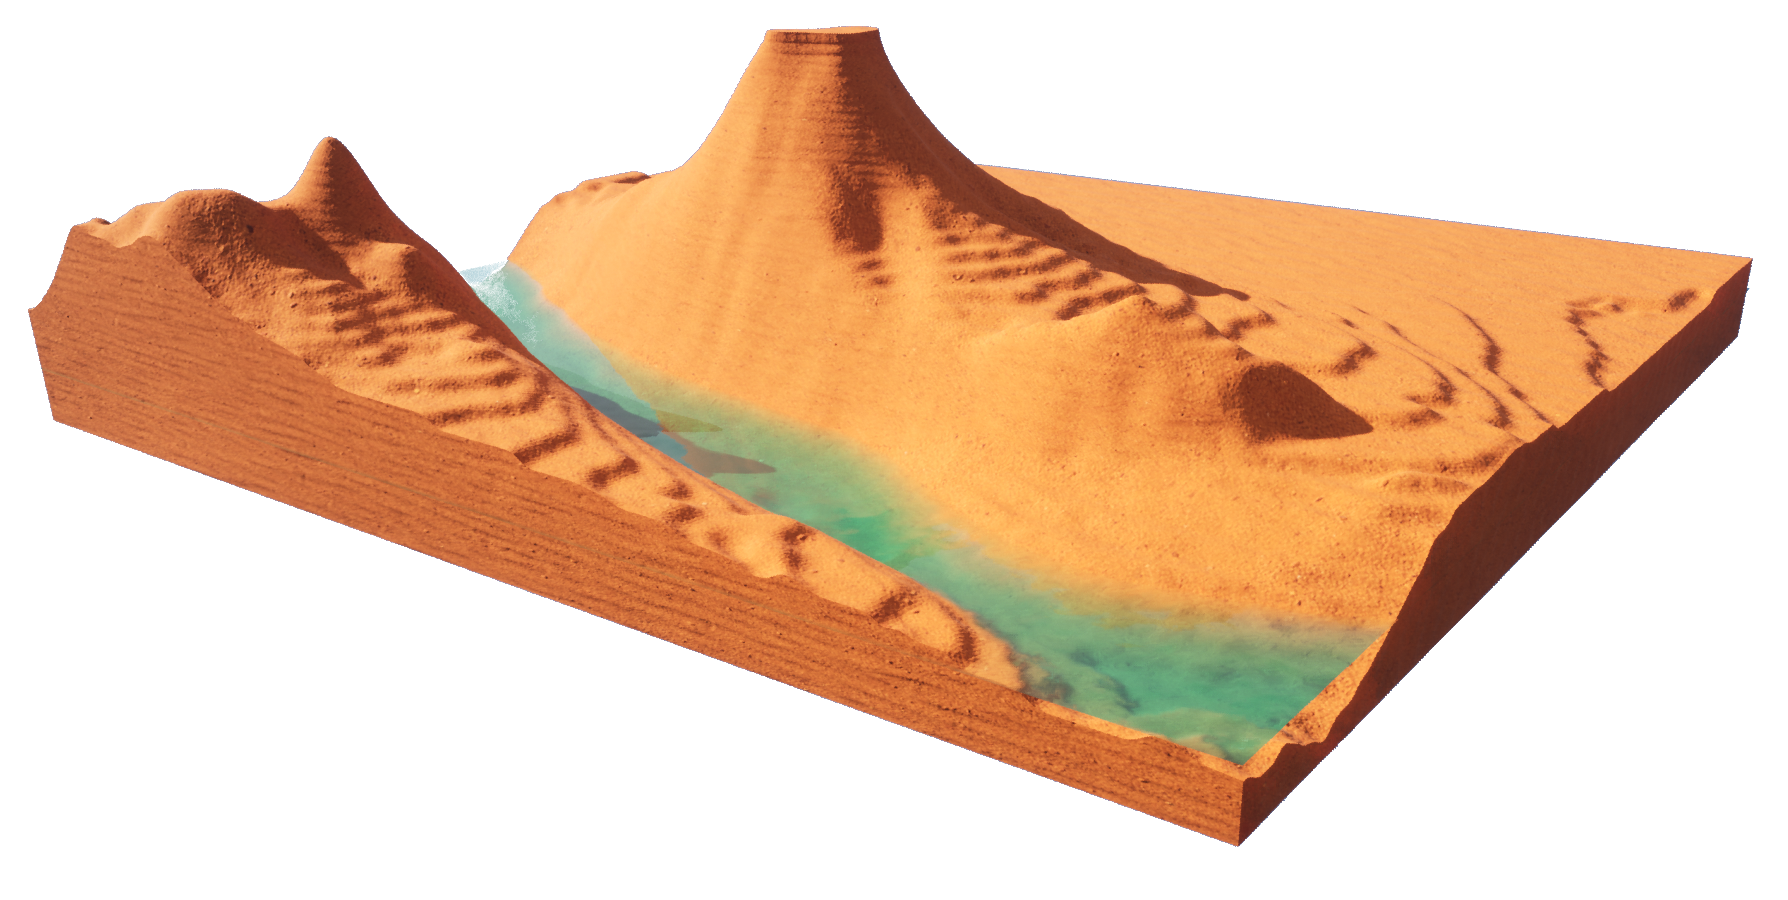
\includegraphics[width=0.49\linewidth]{Results/MultiEffects_base.png}
    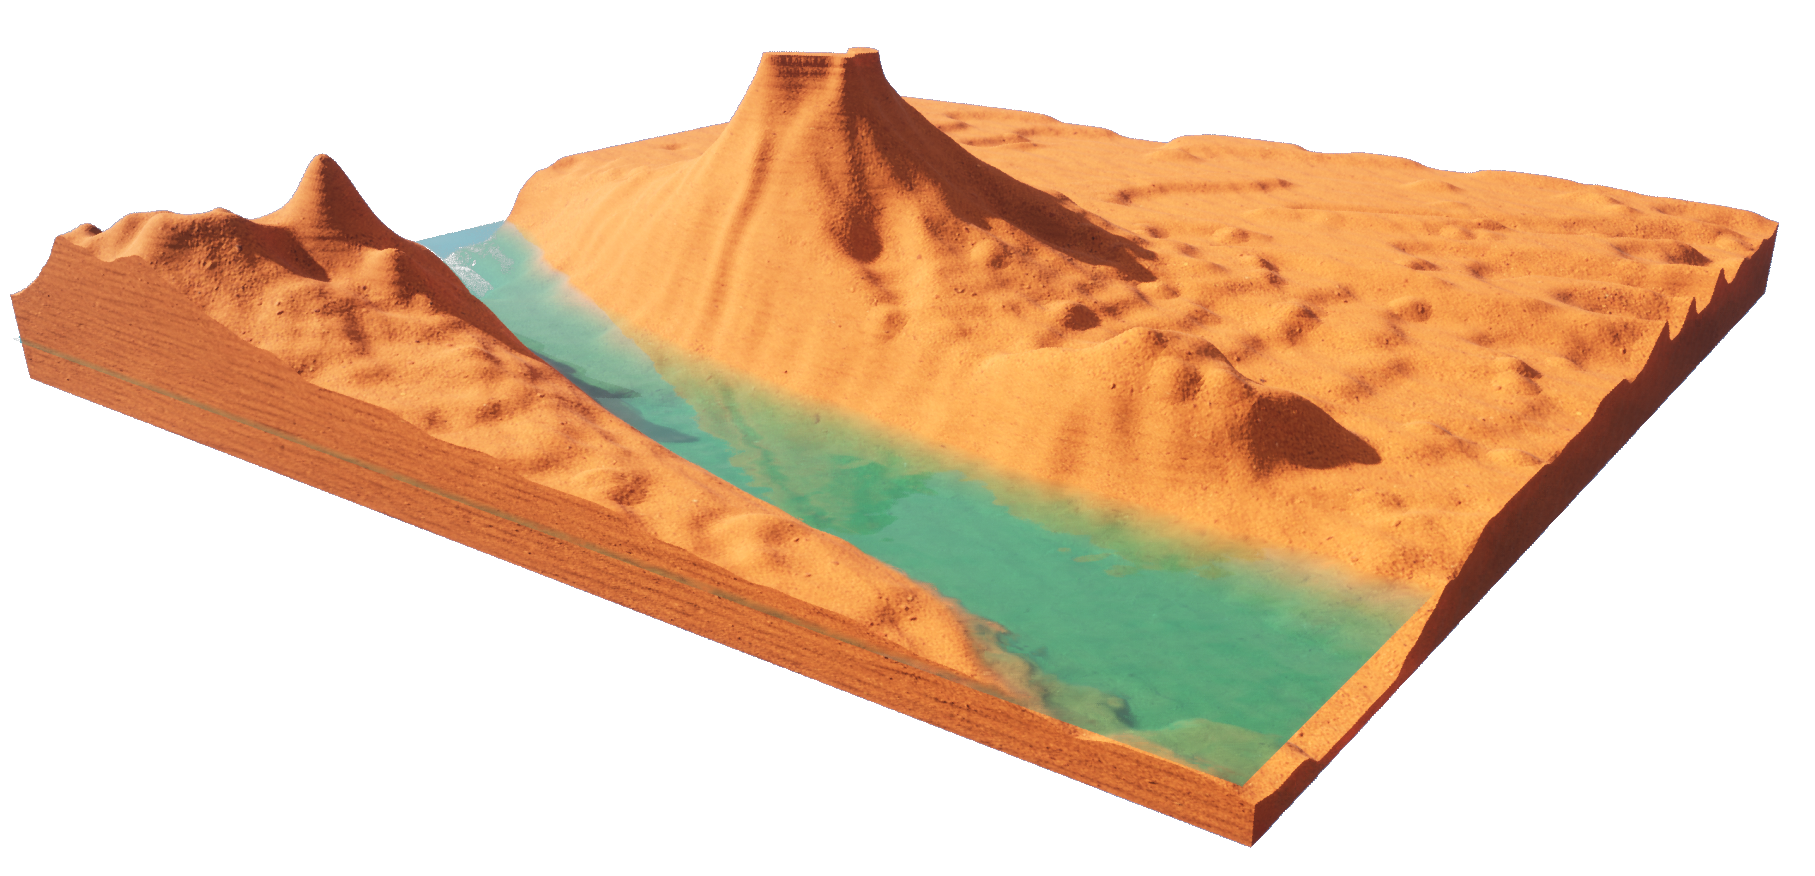
\includegraphics[width=0.49\linewidth]{Results/MultiEffects.png}
    \caption{Multiple erosion types can be combined. On an initial synthetic 500x500x50 density voxel grid, the a wind erosion is applied on the surface of the terrain while hydraulic erosion shapes the rills and the base of the mountains. A water current digs its borders and spreads sediments at the bottom. }
    \label{fig:erosion_multiErosions}
\end{figure}
\textbf{Multiple phenomena} A terrain eroded with multiple erosion phenomena applied on a 500x500x50 density-voxel grid is illustrated in Figure~\ref{fig:erosion_multiErosions}. Here, water-density particles are applying rain on the terrain while the coasts of the river are being eroded thanks to a velocity field defined at the water level. The velocity field defined in the air mainly affects particles with air-density, such that wind erosion can be applied at the same time. The computation of these effects took 7 seconds on CPU.

\textbf{Underwater currents}
Procedural generation of underwater 3D terrains has received little attention. The difference between the underwater and the surface rely on the buoyancy force that is much stronger, meaning that the water flow has a much more impacting effect on erosion than wind. Taking into account the density of the environment and the velocity field of water in our formulas are the keys to be able to apply any erosion in this environment. 
Our method works in a water environment by giving at least water density to particles. Given a velocity field describing underwater currents from a complex simulation or from a sketch, the particle system erodes the terrain. \\ 
In the example presented in \referenceExemple{Underwater}, the velocity field is given by a simple 3D fluid simulation \cite{Stam1999} applied on the terrain.

A complex water flow simulation is computed using SIMPLE \cite{Caretto1973} fluid simulation with OpenFOAM. The resulting erosion can then follow complex water movement and erode the terrain at the most affected parts of the 3D terrain as the trajectories of the particles (green) is highly affected by the fluid velocity (blue). The density of the particles and the environment being close, the buoyancy cancels most of the gravity force, leaving the velocity of the particles computed by the fluid velocity $\fluidVelocity$ and settling velocity $\settlingVelocity$ from \eqref{eq:velocity-computation-final} (Figure~\ref{fig:erosion_underwater_result}).
\begin{figure}[t]
    
    \centering
    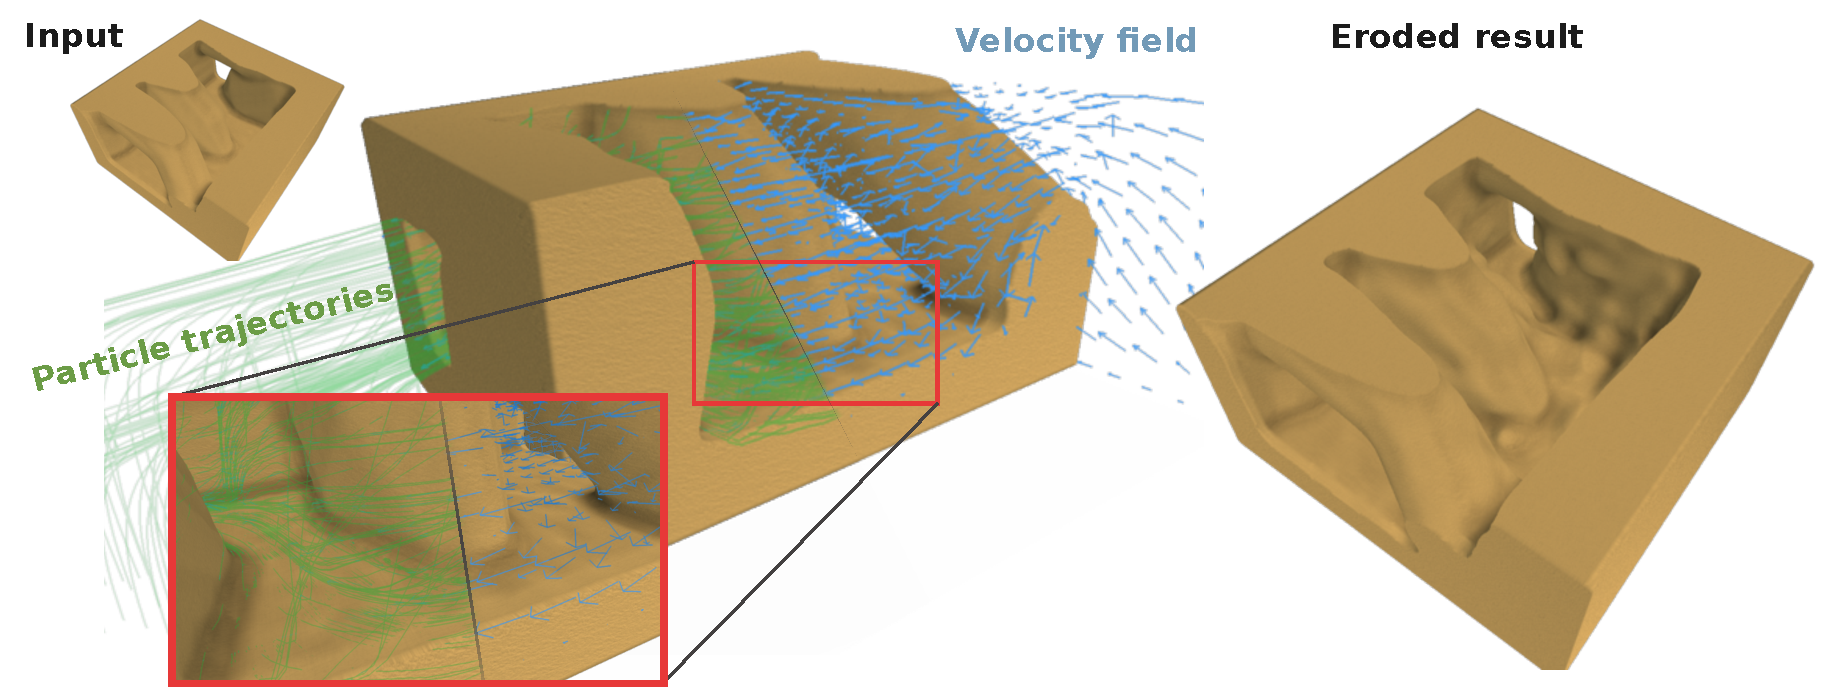
\includegraphics{Results/flowfield.pdf}
    \caption{A complex water flow simulation is computed using OpenFOAM. Particle trajectories (green) are highly affected by the fluid velocity (blue). Most the terrain exposed surfaces is eroded (bottom). }
    \label{fig:erosion_underwater_result}
\end{figure}
% -----------------------------------------------------------------
\section{Comparisons}
In the following section, we compare our method with existing ones to show that while we are versatile on the terrain representation, we are also able to reproduce various effects without applying specific algorithms. The other works are displayed in blue to distinguish them from ours.

\textbf{Coastal erosion on implicit terrain representation:}
Paris et al present an erosion simulation method applied to implicit terrains able to create coastal erosion, karsts and caves by adding negative sphere primitive in the terrain's construction tree \cite{Paris2019}. The positions of the spheres are determined using a Poisson disk sampling at the weakest terrain area defined by the Geology tree of their model. They are simulating the corrosion effect of water on the rocks. Our work is also able to approximate this phenomena by defining the position of these sphere primitives at the position where the water particles hit the surface. While the computation time of the positions of the sphere is higher due to the fact that we are evaluating the position of our particles at every time step in the implicit model (which could be improved by the triangulation of the implicit surface, or better, a dynamic triangulation), the distribution of our erosion primitives is based on a physical model instead of a mathematical model, meaning that we can integrate more easily the direction and strength of the waves for example. The management of their sphere primitives can be replicated with our method by considering that a particle exists until a collision occurs, at which point it disappears. Their method is not conserving the mass of the terrain, which is acceptable for the corrosion simulation, but limits its validity for other erosion simulations. In our method, the particle can be tracked until it settles, ensuring mass conservation (Figure~\ref{fig:erosion_screen-paris2019-1});

\begin{figure}
\centering
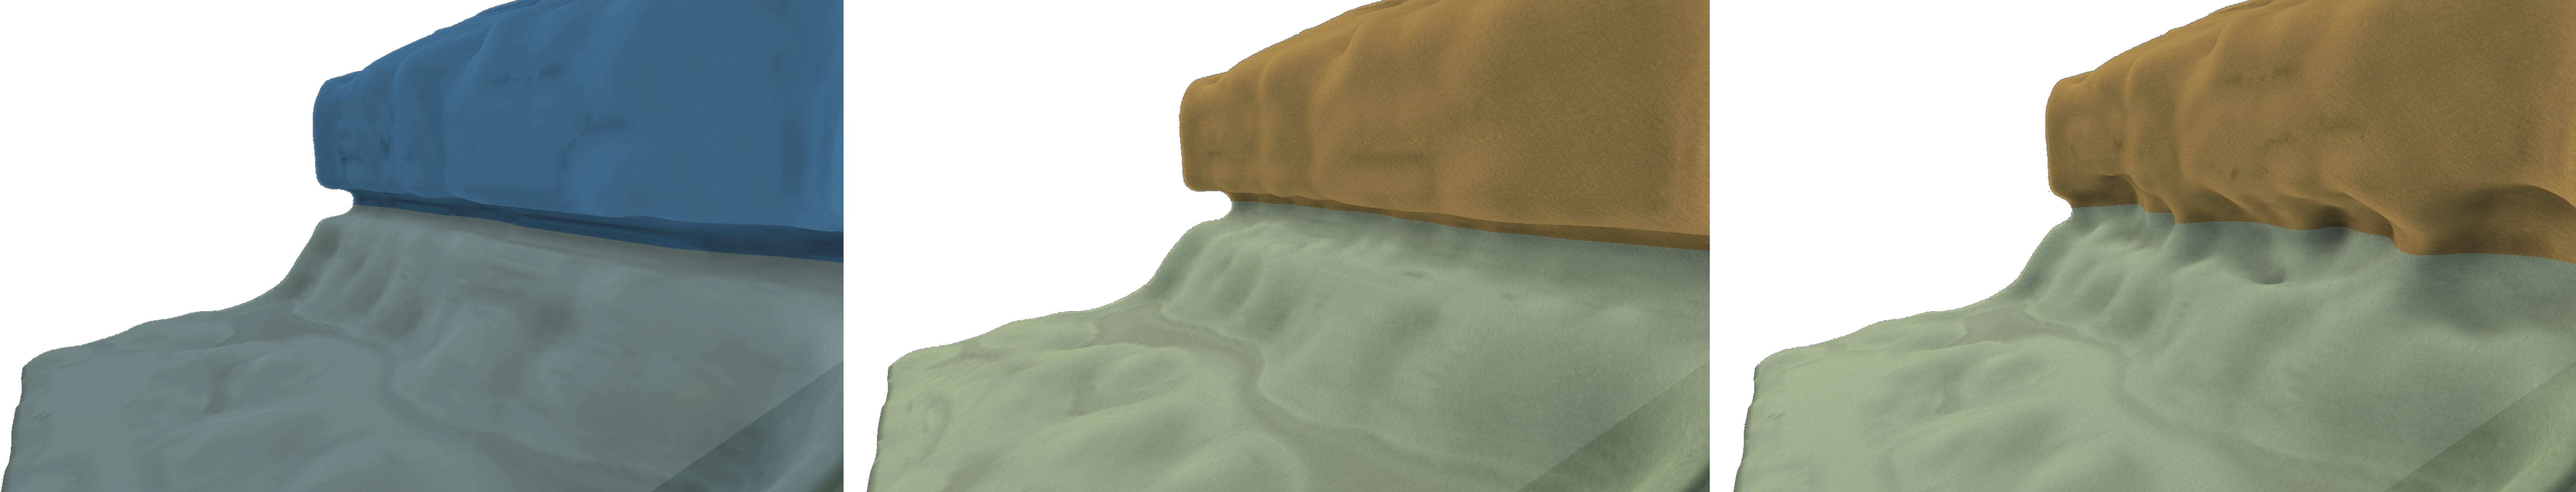
\includegraphics{otherPapersRepro/costal.pdf}
\caption{The algorithm proposed by Paris et al \cite{Paris2019} allows for the simulation of coastal erosion (left) that we can reproduce almost identically by allowing our particles to collide only once with the ground and applying only erosion (center). If we apply our erosion with the full tracking of our particles and using deposition, we can achieve more diverse results (right).}
\label{fig:erosion_screen-paris2019-1}

\end{figure}
%
\begin{figure}[t]

\centering
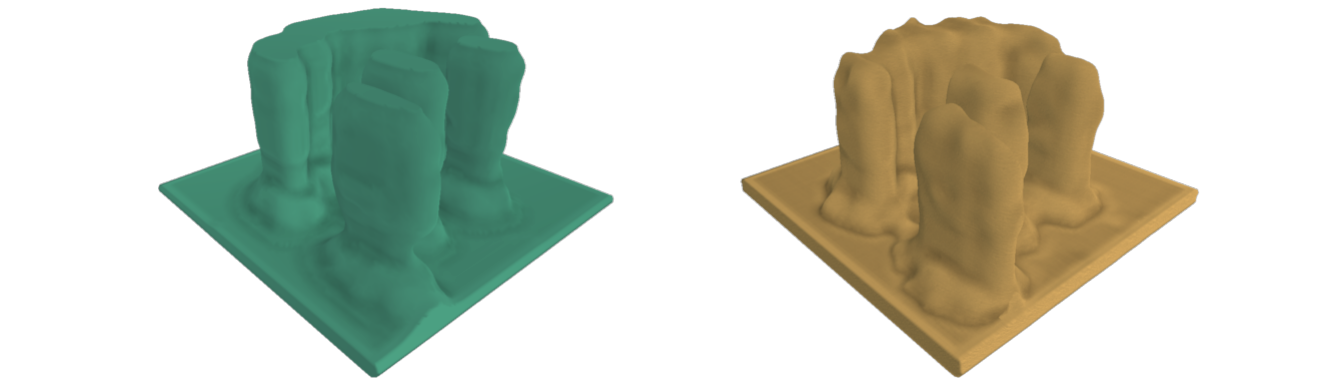
\includegraphics[width = \linewidth]{otherPapersRepro/gobelins2.png}
\caption{The algorithm proposed by Jones et al 
\cite{Jones2010} allows for an efficient simulation of the spheroidal erosion, making the creation of gobelins on voxel grids in a plausible way (left). Our algorithm naturally erodes the most exposed areas of the terrain when particles are affected by the wind (right).}
\label{fig:erosion_screen-jones2010}
\end{figure}
%
\textbf{Wind erosion on voxel grid representation: }
Jones et al propose a weathering erosion on voxel grids by approximating and eroding continuously the most exposed voxels \cite{Jones2010}. When a solid voxel is decimated, it is considered deposit and is displaced down the slope until a minimal talus angle in the terrain is reached and if the deposition is eroded again, it disappears. Our work is able to reproduce their algorithm by sending our particles from a close distance to the terrain surface. By doing so, we reproduce the erosion process as much as the deposition process since the air particles, filled with sediments, is falling automatically towards the local minimum of the erosion point. Just like in their work, we can easily define the resistance value of the materials to add diversity in the results. By adding the possibility of a wind field, even a very simple uniform vector field, to the simulation, we naturally add the wind shadowing effect that protects a gobelin surrounded by bigger gobelins, and also allows the deposit slope to fit more closely to the wind direction (Figure~\ref{fig:erosion_screen-jones2010}).

\begin{figure}[b]
\centering
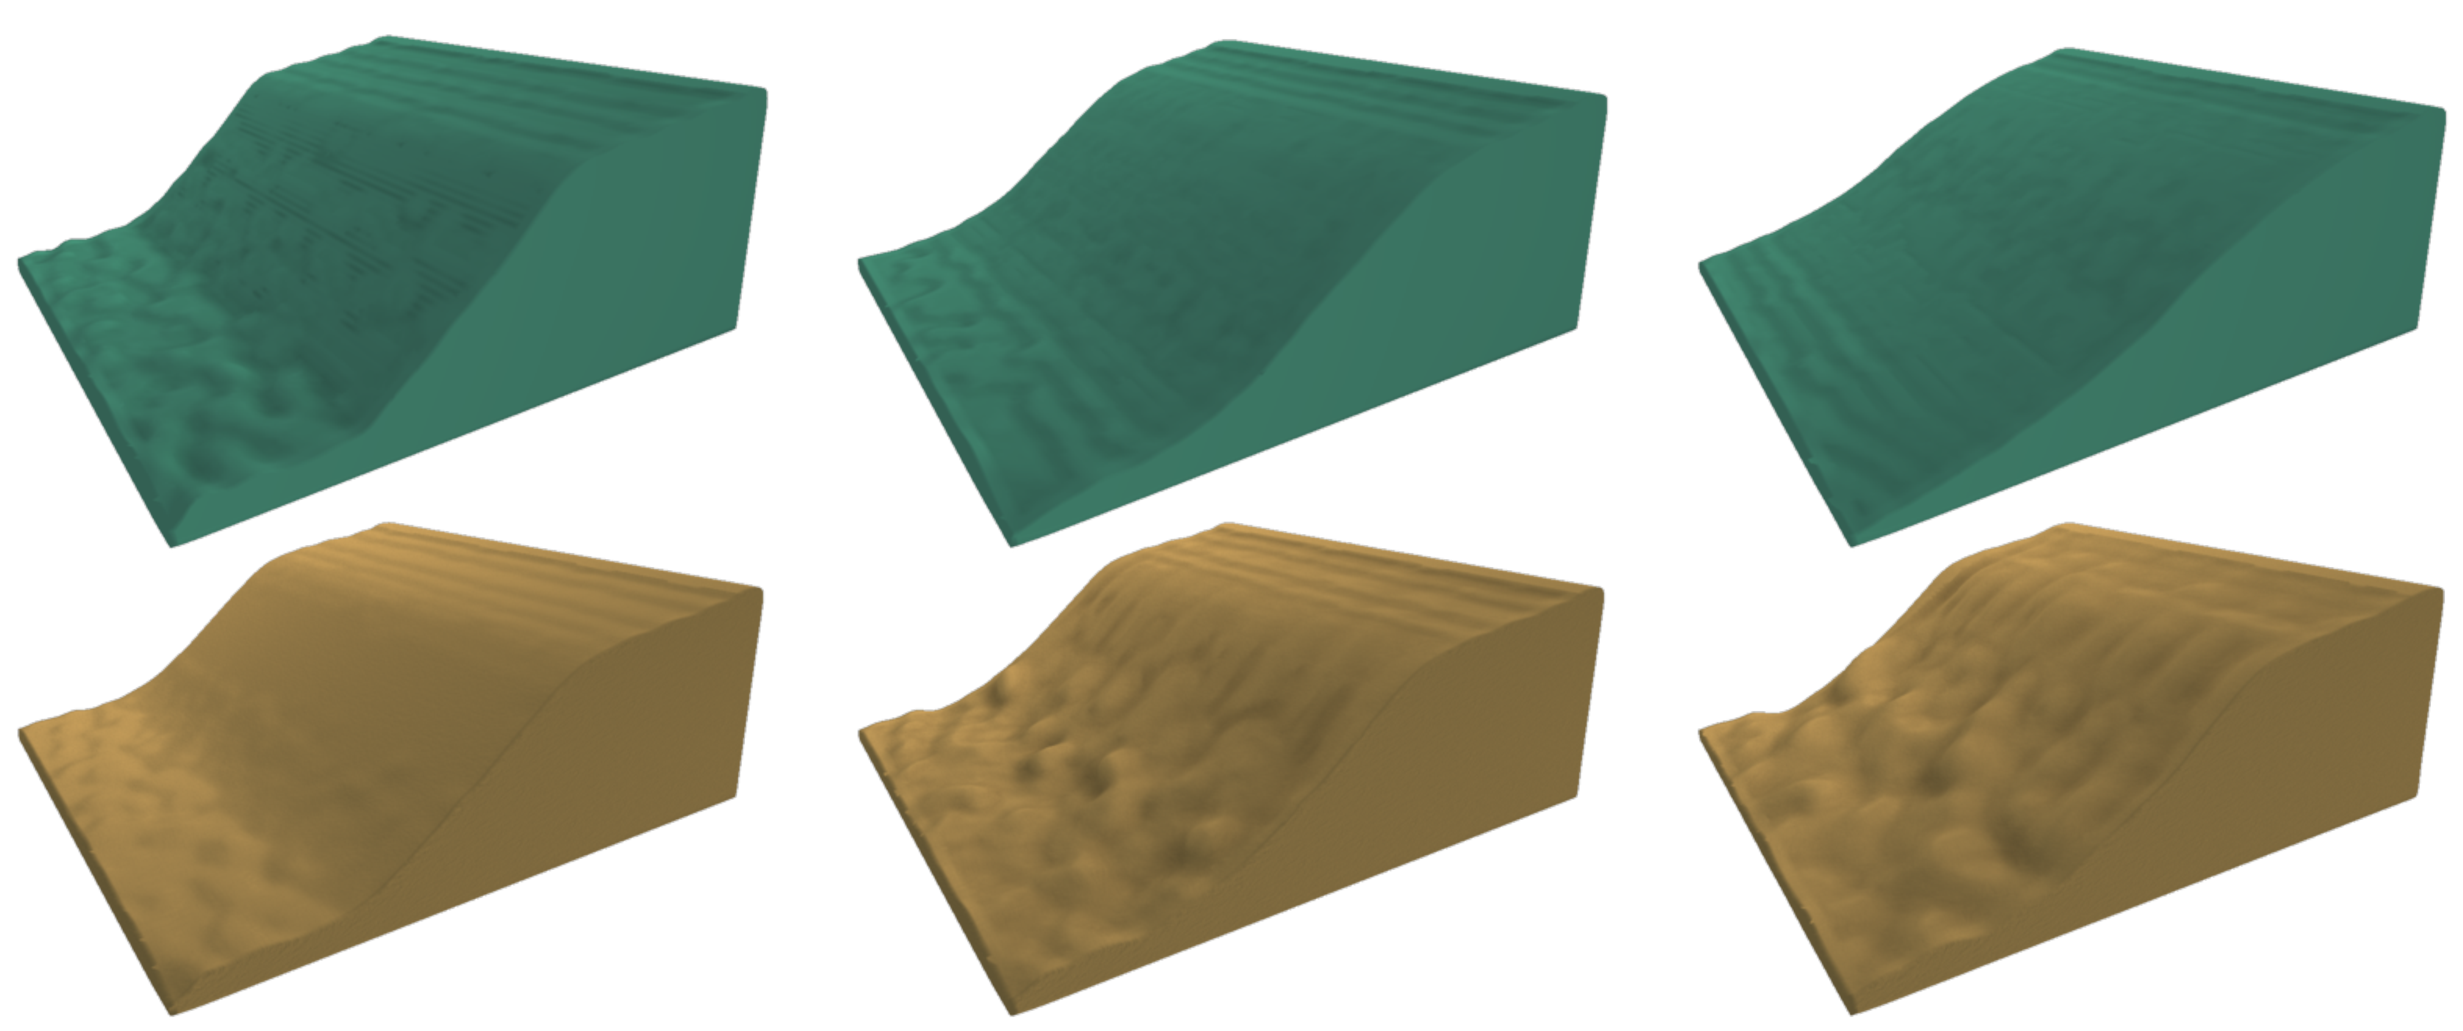
\includegraphics[width= 1\linewidth]{otherPapersRepro/hydro.pdf}
\caption{While our resulting geometry on the hydraulic erosion (bottom) is less smoothed than the one proposed proposed by Mei et al. \cite{Mei2007} (top), our method allows the application on more terrain representations than the height fields only.}
\label{fig:erosion_screen-mei2007-1}

\end{figure}

\textbf{Hydraulic erosion on height field representation: }
Mei et al integrate and adapt to the GPU the pipe model proposed in \cite{OBrien1995} for the fluid simulation \cite{Mei2007}. This simulation is simple but efficient enough to approximate the Shallow-Water equations in real time and use the speed of columns of water to compute the erosion and deposition rate on the 2D grid of the terrain at each time step. Using columns of water even allows the flow to overpass small bumps on the terrain over time. Our method initially rely on a stable fluid flow that is consistent during the whole life time of a particle, but by refining the simulation at each time step instead of at the end of the particles lifetime, our erosion model is able to reproduce this effect, allowing the terrain to have a single batch of fluid going through it. Our method can be seen as a generalization of Mei at al. that can then be used on more than discrete 2D grids (Figure~\ref{fig:erosion_screen-mei2007-1}). 

\textbf{Wind erosion on stacked materials representation: }
Paris et al \cite{Paris2020} simulate the effect of wind over sand fields defined on stacked materials, creating dune structures, even taking into account obstacles like \cite{Roa2004} and different material layers like vegetation \cite{Cordonnier2017a} that are not affected by abrasion\cite{Paris2020}. A wind field simulation is required to produce results, and while \cite{Roa2004} and \cite{Onoue2000} consider a uniform vector field, this work consider a dynamic vector multi-scaled warped field from the terrain height. The sand grains then apply multiple moves: sand lift, bounces, reptation and avalanching. Once the sand is lifted by the wind, the trajectory of the grains can be seen as the displacement of particles, fitting completely with our model as illustrated Figure~\ref{fig:erosion_screen-paris2020}.
\begin{figure}[ht!]
\centering
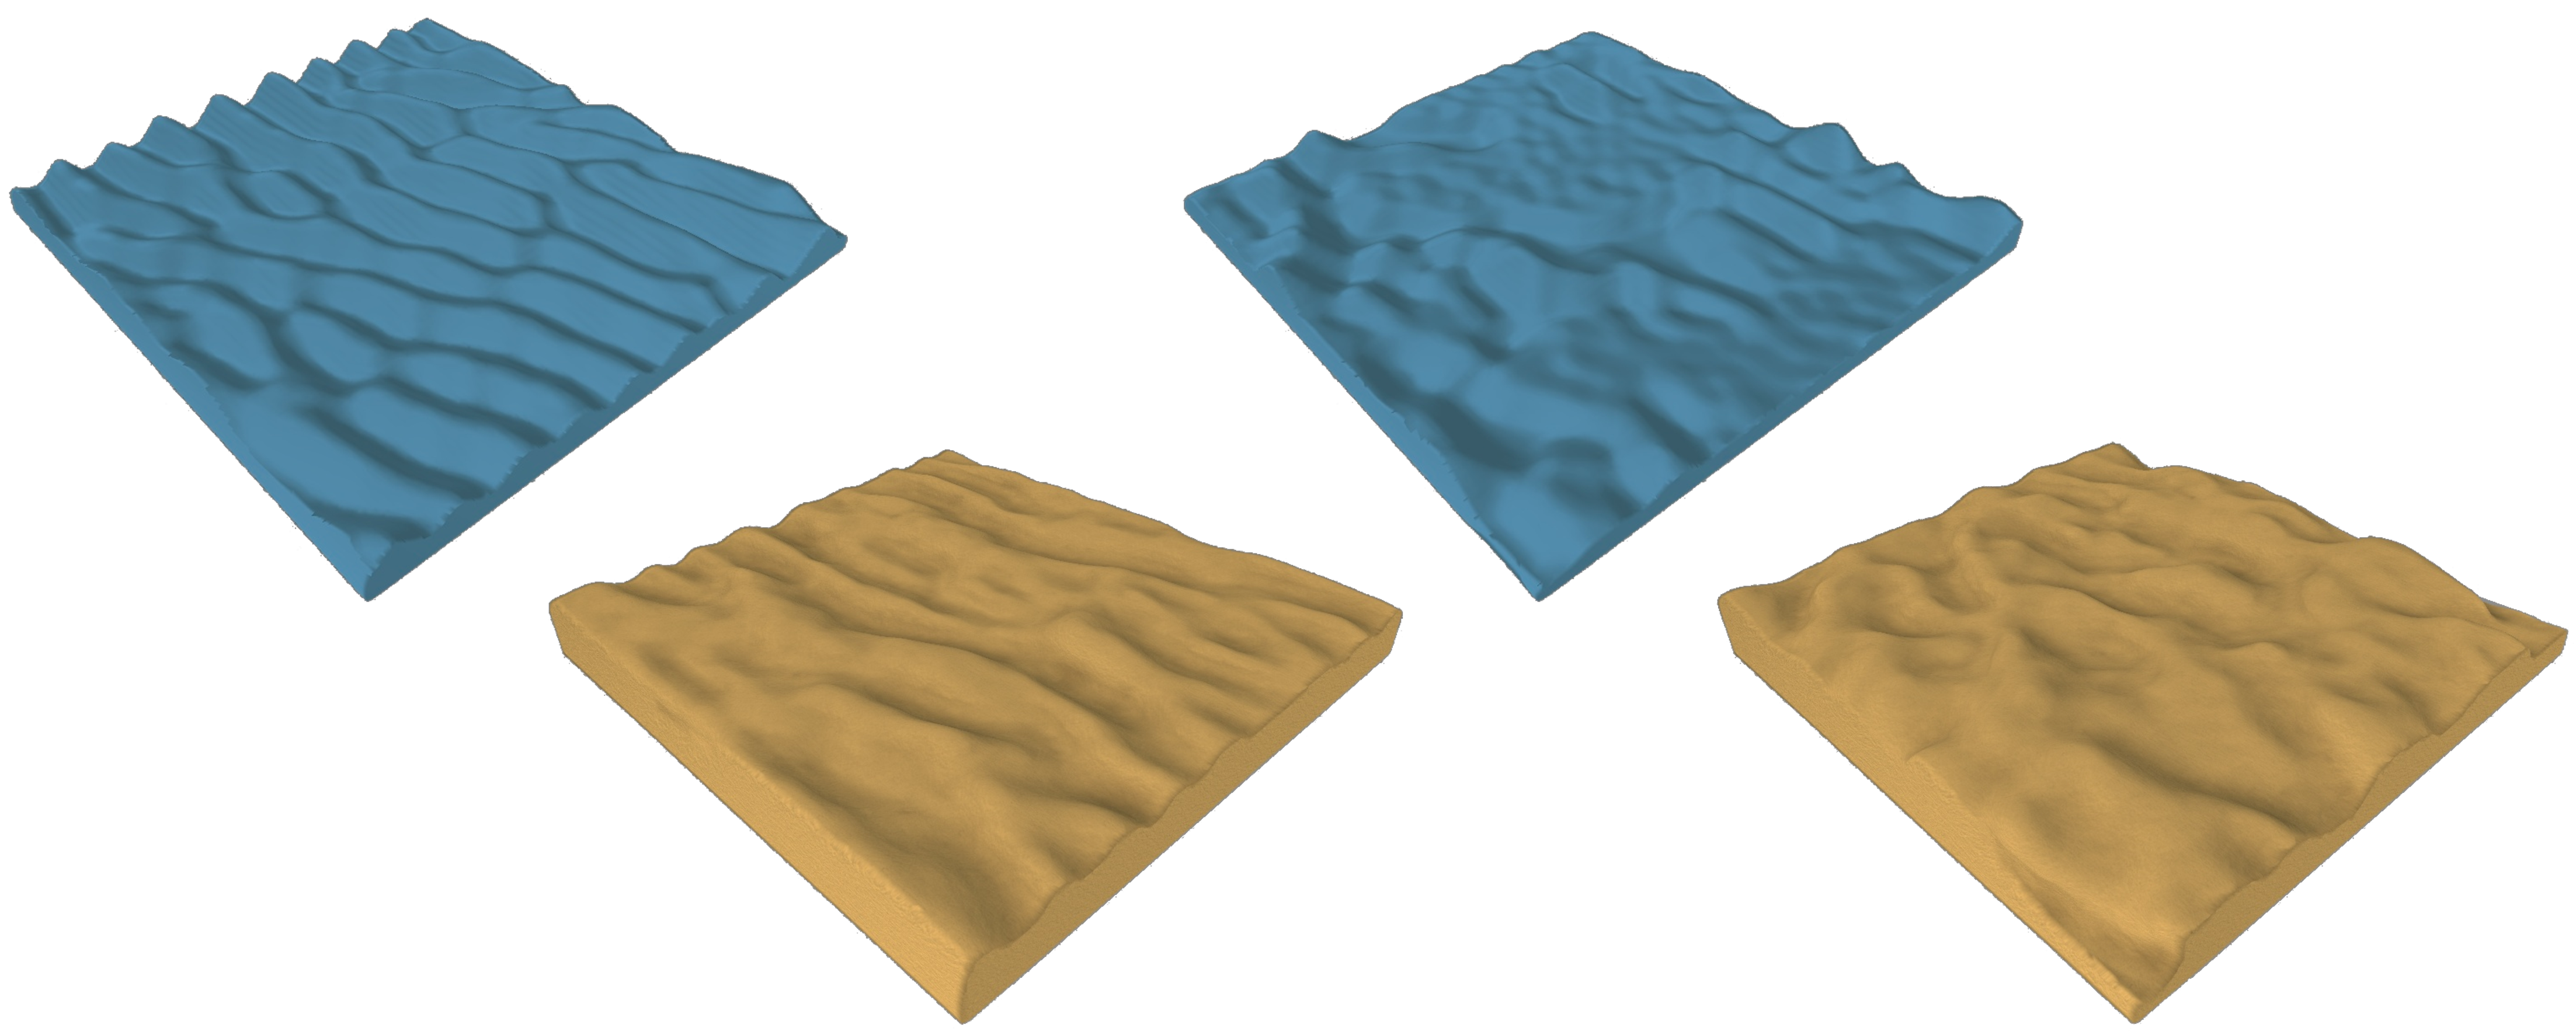
\includegraphics{otherPapersRepro/desert.pdf}
\caption{The algorithm from Paris 2020 allow the generation of desertscapes (top), which we can (at least partially) reproduce with our erosion simulation (bottom). The different effects are achieved by affecting the wind direction and strength. }
\label{fig:erosion_screen-paris2020}
\end{figure}

\section{Discussion}
This work is a generalization of erosion that is applicable to any terrain representation. In practice, while similar particle physics is used on different terrain representations, using similar parameters does not ensure resulting in the same eroded terrain. Surfaces and normals being approximated differently have rippling effect on particle trajectories. 
Note that, not all effects can be applied to all representations, forinstance, karsts generation on 2.5D data structures. 

\textit{Realism}
Realism of the erosion simulation is highly correlated to the size and quantity of particles used and their distribution. Using too few or distributing them too sparsely will result in a terrain that is unrealistic since the alteration will have localized effects, breaking process homogeneity. \\ 
The resolution is also limited by the number and size of the particles, which can be problematic on implicit terrains that can theoretically have a infinite resolution.\\
Our method allows to perform erosion on implicit terrains. However, in its current form, our algorithm is time expensive on implicit representations since a large number of primitives are added in the composition tree. Using skeletons-defined primitives \cite{Hong2013, Rigaudiere2000}%, Schroeder1994}
 from particles trajectories and erosion/deposition values could be a solution to optimize the computation time.

\textit{Usage of velocity fields}
In our erosion algorithm, we simplify particle physics to enhance computational efficiency and facilitate parameterization. We use the velocity field from fluid simulations to approximate particle velocities. Sediment mass is harnessed to compensate for this approximation, allowing compatibility with various fluid simulation algorithms. Velocity fields can be recomputed at a frequency meeting the applications needs, ranging from "classic erosion simulation" (recomputed at each time step) to "simple simulation" (never recomputed). We addressed provisional adjustments to mitigate discrepancies when terrain changes due to erosion are not reflected in a static velocity field in section “3.3 Transport”. However, it is important to note that these are expedient solutions and may not fully capture precise dynamics of an evolving terrain. 

\textit{Performances}
To facilitate parallelization, we intentionally overlook particle interactions and sediment exchanges, albeit at the expense of achieving smoother results. Surface collisions are simplified to basic bounces with a damping parameter instead of relying on complex particles and ground properties (Young's modulus, friction, material, ...)\cite{Yan2020}, further easing the parameterization process. However, these simplifications, combined with the inherent discrete nature of particles, as opposed to the continuous nature of erosion, result in a correlation between realism and particle count. \\
The performance of our method is influenced by the time required for collision detection. Consequently, we mainly observe better performances with explicit terrain models than with implicit models. 

\textit{Particle's atomicity}
While we can replicate various effects, the "fan" shape commonly observed in natural erosion patterns is not perfectly represented. This limitation arises because we do not account for the splitting of a particle, a process that significantly influences the multidirectional dislocation and trajectory of individual particles \cite{Ranz1960}. Additionally, we acknowledge an issue where particles may collide with the ceiling and the deposition is stuck. While a potential resolution involves splitting particles upon impact rather than simply depositing sediments, this introduces complexities to the parallelization layer of the method. Allowing particles to split introduces unpredictability in the total number of particles that will exist in the simulation. This unpredictability can complicate the use of multi-threading. Future works includes finding a data structure allowing this splitting efficiently, leading to more realistic erosion patterns.

\textit{Simulation with multiple materials}
One aspect we haven't addressed is a layered terrain with multiple materials. In the native way our method is done, we do not consider the transport of different materials (all sediments are considered as sand), but by storing a list of the different materials and the quantity transported by each particle, the same simulation process could be done at the cost of some memory and performance overhead. \\
Another possible adaptation of the erosion strategy for material voxels is to extend the erosion computation from binary voxels by define transformation rules from one material to another when a voxel is eroded a number $\#hits < -C$ or $\#hits > C$. For example, the material "clay" may transform to "sand" when eroded or to "rock" when many depositions occurred. 
\section{Conclusion}
\label{sec:erosion_conclusion}
We introduced a flexible particle-based erosion system that is easy to use and simple to implement. We have presented how to adapt the process for various terrain representations and generate a variety of erosion phenomenon due to rain, wind, water bodies... by adjusting intuitive parameters hence generate automatically realistic 2.5D and 3D terrains. The use of external velocity fields provides a high flexibility i.e. using the simulations that best fits the user's needs (precision, control, implementation efficiency...). 
Our method can also be applied to underwater environments with identical physics simulation since our erosion method can be applied on 3D representations. 
Erosion algorithms are often limited to the use of height fields, but by finding more generalized methods, we can go toward a global use of 3D terrains, which can offer richer and more diverse landscapes.

%
\section{Computation of a metaball}
\label{sec:erosion_appendix_metaball}
We use the following formula to evaluate a metaball in space with a center $c$ and of radius $\radius$:
$$ g(\p) = 1 - \frac{||\p - c||}{\radius} $$
using the euclidean distance.

We have a total amount $\totalErosion$ to define in this space, so the final metaball function $f$ needs to satisfy the equations \eqref{eq:function_f_is_metaball} and \eqref{eq:int_function_f_is_erosion}:
\begin{align}
\label{eq:function_f_is_metaball}
f(\p) &= \lambda g(\p) \\
\label{eq:int_function_f_is_erosion}
\int_{\p \in V_{3D}}{f \, dp} &= \totalErosion
\end{align}

First, let's exploit the radial symmetry of the metaball and rewrite $g(\p) = 1 - r$ by using the polar coordinates of the point $\p - c$.

We can then integrate $g$ over the volume $V_{3D}$ as 
\begin{align}
&\int_{0}^{1}{ \int_{0}^{\pi}{ \int_{0}^{2\pi}{ g(r) r^2 \sin(\theta)\, dr} \, d\theta} \, d\phi} \nonumber \\
= &\int_{0}^{1}{ \int_{0}^{\pi}{ \int_{0}^{2\pi}{ (1 - r) r^2 \sin(\theta)\, dr} \, d\theta} \, d\phi} \nonumber \\
&= \int_{0}^{1}{ (1 - r)r^2 \, dr} \times \int_{0}^{\pi}{ \sin{\theta} \, d\theta } \times \int_{0}^{2\pi}{ 1 \, d\phi} \nonumber
\end{align}

We then break down the integrals one by one such as 
$$ \int_{0}^{1}{ (1 - r)r^2 \, dr} = \frac{1}{12} \nonumber$$ 
$$ \int_{0}^{\pi}{ \sin{\theta} \, d\theta } = 2 \nonumber$$ 
$$ \int_{0}^{2\pi}{ 1 \, d\phi} = 2 \pi \nonumber$$

By combining all these integrals, we get $\int{g} = \frac{1}{12} \times 2 \times 2\pi = \frac{\pi}{3}$.

So given $\int{f} = \erosionAmount$ and $\int{f} = \lambda \int{g}$, we can deduce that $\lambda = \frac{\totalErosion}{\int{g}} = \frac{3}{\pi}\totalErosion$.

From \eqref{eq:function_f_is_metaball} we finally get 
\begin{align} 
\label{eq:proofErosionMetaball}
f(\p) = \frac{3 \totalErosion}{\pi} \left(1 - \frac{||\p - c||}{\radius} \right)
\end{align}
, representing the rate of change on the evaluation function of the terrain surface.

The integration in the voxel space is out of the scope of this paper and a numerical solution is instead proposed in Section~\ref{sec:erosion_application_on_voxels}.


\clearpage
\begin{figure*}
	\centering
    \includegraphics{Results/results.pdf}
	\caption{Erosion processes results on various representations presented in section \ref{sec:erosion_erosion_examples}. Used parameters used are detailed in  Table~\ref{tab:result_parameters}.}
	\label{tab:result_figures}
\end{figure*}


%\chapter{Érosion continue}
\label{chap:continuous-erosion}
\minitoc

- ...

\section{Description du problème}
\label{sec:continuous-erosion_problematic}
- Processus d'érosion est un système dynamique \\
- Nombre de variables très important \\
- Impossible de simuler à des pas de temps différents et/ou à différentes échelles/résolutions

\section{Solutions proposées}
\label{sec:continuous-erosion_solutions}
- ...

\subsection{Utilisation d'apprentissage profond}
- ...


\backmatter
\chapter*{Conclusion}
\addcontentsline{toc}{chapter}{Conclusion}
- ...

\pagenumbering{Roman}

%\bibliographystyle{eg-alpha-doi}
%\bibliographystyle{siam}
%\nocite{*}
\addcontentsline{toc}{chapter}{References}
\printbibliography[title=References]
%\bibliography{../references_terrain}



% \include{chapitre1}
%%%%%%%%%%%%%%%%%%%%%%%%%%%%%%%%%%%%%%%%%%%%%%%%%%%%%%%%%%%%%%%
\end{document}